% Project Management Plan Documentation Template %
% Template made following ISO/IEC/IEEE 16326:2009 %

% Author : Alejandro Muñoz Del Álamo %
% Copyright 2019 %

% Main File %

% Define document type 
\documentclass[a4paper, 11pt, dvipsnames]{book}

% Declaration of packages for this document
\usepackage[utf8]{inputenc}
\usepackage[spanish]{babel}
\usepackage{titlesec}
\usepackage{xcolor}
\usepackage{float}
\usepackage[hidelinks]{hyperref}
\usepackage{bookmark}
\usepackage{graphicx}
\usepackage{emptypage}
\usepackage{eurosym}
\usepackage{geometry}
\usepackage[autopunct]{csquotes}
\usepackage{ragged2e}
\usepackage{longtable,tabularx,array}
\usepackage{multirow}
\usepackage{fancyhdr}
\usepackage{spreadtab}
\usepackage{fp}
\usepackage{changepage}
\usepackage{epigraph}
\usepackage{array}
\usepackage{lscape}
\usepackage{makecell}
\usepackage{enumitem}
\usepackage{svg}
\usepackage{amsmath}
\usepackage[Sonny]{fncychap}
\usepackage{nameref}
%Options: Sonny, Lenny, Glenn, Conny, Rejne, Bjarne, Bjornstrup
\usepackage{tocbibind}
\usepackage{tocloft}
\usepackage[bottom]{footmisc}
\usepackage[skip=2pt]{caption}
\usepackage{booktabs}
\usepackage[sorting=none]{biblatex}
\addbibresource{ARPEGOS.bib}

% Declaration of quoting commands
%\SetCiteCommand{\parencite}


% Declaration of epigraph details
\renewcommand{\epigraphflush}{center}
\setlength{\epigraphwidth}{10cm}

% Declaration of makecell commands
\renewcommand{\cellalign}{\theadalign{cl}}
\renewcommand\theadfont{\bfseries}
\renewcommand\theadgape{\Gape[2pt]}
\renewcommand\cellgape{\Gape[2pt]}

% Declaration of global commands

\newcommand{\vsep}{\hfil\kern\arraycolsep\vline\kern-\arraycolsep\hfilneg}
\newcommand{\dotnet}{.NET}
\newcommand{\blankpage}
{
    \checkoddpage{}
    \ifoddpage{\newpage}{} \fi
    \cleardoublepage{}
    \thispagestyle{empty}
    \newpage
}

\newcommand{\DNI}{77396804-X}
\newcommand{\autor}{Alejandro Muñoz Del Álamo}
\newcommand{\director}{D. Alberto Gabriel Salguero Hidalgo}
\newcommand{\codirector}{D. Pablo García Sánchez}
\newcommand{\proyecto}{ARPEGOS\@: Automatized Roleplaying-game Profile Extensible Generator Ontology based System}
\newcommand{\nombre}{ARPEGOS}
\newcommand{\tipo}{Grado} % Grado / Máster %
\newcommand{\titulo}{Ingeniería Informática}
\newcommand{\titulacion}{\tipo{} en \titulo}
\newcommand{\dia}{14}
\newcommand{\mes}{Febrero}
\newcommand{\anno}{2020}
\newcommand{\fecha}{\mes{} \anno}
\newcommand{\Fecha}{\dia{} de \mes{} de \anno}

\newcommand{\lorem}
{
    Lorem ipsum dolor sit amet, consectetur adipiscing elit. 
    Nullam maximus facilisis odio vel dignissim. Integer sed tincidunt neque. 
    Cras vitae nisi odio. Morbi in pellentesque nulla. 
    Nam sagittis leo nec ex ultricies, eget hendrerit velit tincidunt. 
    Phasellus fringilla varius tellus, in aliquam purus convallis eget. 
    Donec mattis nisi turpis, vitae ultrices lectus ornare at. 
    Lorem ipsum dolor sit amet, consectetur adipiscing elit. Duis in rutrum eros. 
    Duis ut lacinia justo. Donec fringilla velit eu sem congue cursus. 
    Etiam porttitor, justo gravida porttitor ultrices, eros sem lacinia ex, 
    eget bibendum enim dolor non ligula. Lorem ipsum dolor sit amet, 
    consectetur adipiscing elit.
}

\newcommand{\protege}{\textit{Protégé} }
\newcommand{\anima}{\textit{Ánima} }

% Plain stylepage Definition %
\fancypagestyle{plain}
{
    \fancyhf{} 
    \renewcommand{\headrulewidth}{0pt}
    \renewcommand{\footrulewidth}{0pt}
}

\fancypagestyle{prefacepage}
{
    \fancyhf{} 
    \renewcommand{\headrulewidth}{0pt}
    \fancyfoot[RE,LO]{\textsl{\thepage}}

}

\fancypagestyle{chapterpage}
{
    \fancyhf{} 
    \renewcommand{\headrulewidth}{0pt}
    \fancyfoot[RE,LO]{}
}

% Header Definition %
\setlength{\headheight}{15pt}
\fancyhead[LO]{\textbf{\textsl{\leftmark}}}
\fancyhead[LE]{\textbf{\textsl{\thepage}}}
\fancyhead[RO]{\textbf{\textsl{\thepage}}}
\fancyhead[RE]{\textbf{\textsl{\rightmark}}}
\fancyhead[C]{}


% Footer Definition %
\fancyfoot[LE,RO]{}
\fancyfoot[LO,RE]{}
\fancyfoot[RE,LO]{}
\fancyfoot[RO,LE]{}
\fancyfoot[C]{}

% Environment Definition %
\newenvironment{portada}
{
    \newgeometry{left=2cm,right=2cm,top=2cm,bottom=1cm}
    \includegraphics[width=7cm, keepaspectratio]{Images/UCA.jpg}  \\ \vspace{1cm}
    \begin{center}
}
{
    \end{center}
    \restoregeometry{} 
}

\begin{document}
    % Title Page  %
    \begin{titlepage} % Portada del documento %
        \newgeometry{left=2cm,right=2cm,top=2cm,bottom=1cm}
        \includegraphics[width=7cm, keepaspectratio]{Images/UCA.jpg}  \\ \vspace{1cm}
        \begin{center}
            \Large \MakeUppercase{Trabajo de Fin de Grado} \\ \vspace{1cm}
            \Large \MakeUppercase{\titulacion} \\ \vspace{6cm}
            \LARGE \MakeUppercase{\textbf{\proyecto}} \\ \vspace{7cm}
            \Large \MakeUppercase{Autor: \autor} \\ \vspace{0.5cm}
            Puerto Real, \fecha{}
        \end{center}
        \restoregeometry{}
    \end{titlepage} % Fin de portada

    \blankpage{}

        % Second Title Page %
    \begin{portada}
        \Large \MakeUppercase{Trabajo de Fin de Grado} \\ \vspace{1cm}
        \Large \MakeUppercase{\titulacion} \\ \vspace{6cm}
        \LARGE \MakeUppercase{\textbf{\proyecto}} \\ \vspace{7cm}
        \Large \MakeUppercase{Director: \director} \\
        \Large \MakeUppercase{Codirector: \codirector} \\
        \Large \MakeUppercase{Autor: \autor} \\ \vspace{0.5cm}
        Puerto Real, \fecha{}
    \end{portada}

    \blankpage{}
    %\frontmatter{}
    \pagenumbering{Roman}
    \pagestyle{fancy}
    % Import Signature
    \input{Documentation-Scheme/Portada/Signature.tex}
    \blankpage{}
    
    % Import Preface
    % Project Management Plan Documentation Template %
% Template made following ISO/IEC/IEEE 16326:2009 %

% Author : Alejandro Muñoz Del Álamo %
% Copyright 2019 %

% Preface File %

% Greeting Clause  % 
{\large \textbf{\textit{Agradecimientos}}}
\lorem

\blankpage

% Documentation License Page %
{\large \textbf{Licencia}}\\

\textit{Copyright} \textcopyright 2019 \autor, todos los derechos reservados.

Las licencias de las imágenes de terceros se especifican en su uso. \newline

Los logotipos de empresas e instituciones que aparecen en este
documento son propiedad de dichas empresas e instituciones, y quedan bajo la licencia
establecida por estas. \newline

La plantilla de este documento ha sido creada por Alejandro Muñoz Del Álamo bajo 
Licencia MIT (GNU \textit{Massachussetts Institute of Technology}) y con 
\textit{copyright }\textcopyright 2019 Alejandro Muñoz Del Álamo, en los términos siguientes.
\textit{"Permission is hereby granted, free of charge, to any person obtaining a copy of 
this software and associated documentation files (the "Software"), to deal in the Software 
without restriction, including without limitation the rights to use, copy, modify, merge, 
publish, distribute, sublicense, and/or sell copies of the Software, and to permit persons 
to whom the Software is furnished to do so, subject to the following conditions:

The above copyright notice and this permission notice shall be included in all copies or 
substantial portions of the Software."}

\blankpage

% Notation & Format Page % 
{\large \textbf{Notación y formato}} \\

En la siguiente tabla se presenta un conjunto de convenios de notación de sintaxis.\\ 

\begin{tabular}{|l|l}
    \hline \multicolumn{2}{|c|}{Notación establecida} \\ \hline
    \textbf{negrita} & Título o texto destacado \\ \hline 
    \textit{cursiva} & Texto en otro idioma, destacado, citas o nombres de aplicaciones \\ \hline
    \texttt{monoespaciado} & Referencias a código fuente \\ \hline
    \underline{subrayado} & Advertencia para el lector \\ \hline
    color & Enlace interno (rojo) \\ \hline
\end{tabular}


    \blankpage{}
    
    \pagestyle{fancy}

    % Import Table of Contents
    \tableofcontents
    \blankpage{}
    
    % Import List of Figures
    \listoffigures
    \blankpage{}
    
    % Import List of Tables
    \listoftables 
    \blankpage{}
    
    %\mainmatter{}
    \pagenumbering{arabic}
    \pagestyle{fancy}

    % Import Part I
    % ARPEGOS:  Automatized Roleplaying-game Profile Extensible Generator Ontology based System %
% Author : Alejandro Muñoz Del Álamo %
% Copyright 2019 %

% Part 1: Prolegómeno %
\part{Prolegómeno}

% Import Chapter 1 %
% ARPEGOS:  Automatized Roleplaying-game Profile Extensible Generator Ontology based System %
% Author : Alejandro Muñoz Del Álamo %
% Copyright 2019 %

% Chapter 1: Introducción %

\chapter{Introducción}
\thispagestyle{chapterpage}

% Import Section 1.1 %
% ARPEGOS:  Automatized Roleplaying-game Profile Extensible Generator Ontology based System %
% Author : Alejandro Muñoz Del Álamo %
% Copyright 2019 %

% Section 1.1: Motivación %

\vspace*{\fill}
\epigraph{\textit{“En Arrswyd, la oscuridad ha consumido las estrellas en el cielo, 
dejando nada más que una sola ciudad en medio del olvido. Arrswyd es una nación amurallada 
donde permanece la última población del mundo. El día ha sido olvidado hace mucho tiempo, 
los miedos se hacen realidad, y entre las torcidas espirales, merodeando entre las sombras, 
hay horrores que se alimentan del miedo. El terror es todo lo que Arrswyd sabe ya que su gente 
es perseguida por criaturas y oprimida por el Señor inmortal, Yomon Ecuro. Algunos se animan a 
luchar contra el abismo y las maquinaciones del Ministerio y del Instituto, mientras que otros 
simplemente quieren vivir los últimos días del mundo hasta que se apague la última luz.”}}{\textit{Arrswyd, Regnum Ex Nihilo}}
\vspace*{\fill}

\newpage

\section{Motivación}
Los juegos de rol, a los que llamaremos \textbf{\textit{RPG}} (\textit{\textbf{R}ole-\textbf{P}laying \textbf{G}ame}) a 
partir de ahora, son juegos con una meta particular, que es \textit{“El objetivo de ambos tipos de juegos, computerizados y 
de otro tipo, es experimentar una serie de aventuras en un mundo imaginario, a través de un personaje avatar o un pequeño grupo de 
personajes cuyas habilidades y poderes crecen conforme el tiempo pasa.”} \autocite*{Adams2010}. 

Uno de los aspectos más importantes de los \textit{RPG} son los personajes, ya que estos son la manifestación de los jugadores 
dentro del universo del juego. Como dicen Ramos y Sueiro~\autocite*{Ramos-Villagrasa2010}, a diferencia del teatro, donde la elección de un personaje puede depender de las características 
físicas del intérprete, en los juegos de rol cualquier persona puede interpretar cualquier personaje, siempre que esté dentro de las 
posibilidades que ofrezca el juego en que se esté jugando. Los personajes deben definirse dentro de los limites establecidos por 
las reglas del juego, y en una historia como si se tratara de su biografía, explicando cómo ha sido la vida del personaje en 
la ambientación hasta el momento de comenzar la historia. A este proceso de definir un personaje 
para un jugador se conoce como \textbf{creación de personaje}. \medskip

Hay un amplio rango de posibilidades cuando tratamos la creación de personajes en diferentes mundos. En algunos juegos, el jugador 
sólo puede seleccionar algunas características predefinidas para el personaje, mientras que en otros juegos el usuario puede cambiar cada
elemento del avatar \autocite*{Isaksson2012}. Esto hace que la creación de personajes sea un proceso arduo y complejo, pues es necesario 
tener amplios conocimientos del juego para conocer todas las opciones de personalización disponibles para el jugador, y sus correspondientes 
características. \medskip

% Hablar del proceso de creación %


El autor del blog \textit{Ars Rolica}~\autocite*{ArsRolica} comenta que una de las novedades que se están popularizando más es la de los 
generadores de personajes, que son herramientas que permiten crear personajes de juegos sin necesidad de invertir grandes cantidades 
de tiempo, evitando posibles errores y deslices. Estos generadores pueden ser bastante útiles tanto para jugadores novatos que no 
conocen el sistema del juego, como para jugadores más experimentados que no puedan utilizar tiempo para documentarse completamente 
antes de crear su álter ego. \medskip

El objetivo de este proyecto consiste en diseñar e implementar un generador de personajes de juegos de rol de mesa, para lo que se 
perseguirán los siguientes subobjetivos:
\begin{itemize}

    \item Realizar un estudio del arte de los generadores de personaje existentes, que permita conocer el estado actual de las herramientas
    que se encuentran en uso en la actualidad.

    \item Desarrollar un sistema que permita trabajar con diferentes juegos de rol, sin tener que salir de la aplicación, siempre y 
    cuando se disponga de los ficheros que contengan la información de dichos juegos.

    \item Diseñar un esquema del sistema de información que permita a la aplicación poder adaptarse de la forma más completa posible a 
    cada juego, permitiendo profundizar de la misma manera en juegos de alta complejidad que en juegos sencillos.

    \item Crear una interfaz de usuario intuitiva, que facilite al usuario la interacción con la aplicación y ésta resulte cómoda y 
    agradable de utilizar.

\end{itemize}









% Import Section 1.2 %
% ARPEGOS:  Automatized Roleplaying-game Profile Extensible Generator Ontology based System %
% Author : Alejandro Muñoz Del Álamo %
% Copyright 2019 %

% Section 1.2: Alcance %
\section{Alcance} \label{Alcance}
Este proyecto consiste en una aplicación que permita al usuario generar fichas técnicas de personajes para 
poder participar en partidas o campañas de \textit{RPG}. La aplicación debe servir para poder desarrollar 
personajes de cualquier juego, siempre y cuando disponga de la información del mismo, pero a su vez debe 
poder explorar todas las posibilidades de cada juego, sin importar su complejidad. \medskip

El objetivo principal que se desea conseguir con esta aplicación es facilitar a todos los jugadores de rol una 
herramienta que facilite la comprensión del proceso de creación de personajes y reduzca la duración del mismo,
pero sin dejar de valorar todas las opciones que el juego pone a su disposición. \medskip

El otro objetivo de este proyecto es desarrollar una herramienta general que pueda ser útil para cualquier \textit{RPG},
independientemente del sistema de creación de personajes que utilice, pues no resulta práctico tener que disponer de 
un \textit{generador de personajes} por cada \textit{RPG} que existe, ya que el coste espacial de disponer de todos ellos 
resultaría imposible de contener en una herramienta de gama media, de forma que no estaría disponible para todos los jugadores.
\medskip

Para conseguir esto, se ha considerado que, en vez de contemplar como objetivo la creación de una base de datos que 
contenga la información de un juego concreto, se va a fijar como meta el diseño de una estructura general para que 
cualquier persona que quiera introducir la información de un nuevo juego, tenga a su disposición una metodología clara 
para desarrollar el banco de datos de manera que la aplicación sea capaz de trabajar con éste.


% Import Section 1.3 %
% ARPEGOS:  Automatized Roleplaying-game Profile Extensible Generator Ontology based System %
% Author : Alejandro Muñoz Del Álamo %
% Copyright 2019 %

% Section 1.3: Glosario de Términos %
\section{Glosario de Términos}
\begin{itemize}

    % Añadir WebSemántica

    \item \textbf{\textit{Android}}: Sistema operativo que se emplea 
    en dispositivos móviles, por lo general con pantalla táctil. 
    De este modo, es posible encontrar tabletas, teléfonos móviles 
    y relojes equipados con Android, aunque el software también 
    se usa en otros dispositivos. 
    % https://definicion.de/android/ 

    \item \textbf{\textit{Blazegraph}}: Base de datos de grafos de 
    código abierto, escalable y de alto rendimiento basada en 
    estándares. Escrito completamente en \emph{Java}, la plataforma soporta 
    las familias de especificaciones \emph{Blueprint} y \textbf{RDF}/\textbf{SPARQL 1.1}
    incluyendo consultas, actualizaciones, consultas federadas básicas
    y descripción de servicios. 
    % https://wiki.blazegraph.com/wiki/index.php/About_Blazegraph
    
    \item \textbf{\textit{C\#}}: Lenguaje de programación multiparadigma 
    desarrollado y estandarizado por Microsoft como parte de su 
    plataforma \textbf{\dotnet}, que después fue aprobado como un estándar por la
    ECMA (\emph{ECMA-334}) e ISO (\emph{ISO/IEC 23270}). 
    C\# es uno de los lenguajes de programación diseñados para la 
    infraestructura de lenguaje común. Su sintaxis básica deriva de 
    \emph{C/C++} y utiliza el modelo de objetos de la plataforma \\dotnet, 
    similar al de \emph{Java}, aunque incluye mejoras derivadas de otros lenguajes.
    % https://es.wikipedia.org/wiki/C_Sharp


    \item \textbf{\textit{RDFSharp}}: \emph{Framework} de código 
    abierto \textbf{C\#} diseñado para facilitar la creación de 
    aplicaciones \emph{\dotnet} basadas en el modelo \textbf{RDF}, 
    que representa una solución didáctica directa para comenzar 
    a trabajar con conceptos de \emph{Semántica Web}.
    % https://www.w3.org/2001/sw/wiki/RDFSharp

    \item \textbf{\textit{Git}}: Software de control de versiones 
    diseñado por \emph{Linus Torvalds}, pensando en la eficiencia 
    y la confiabilidad del mantenimiento de versiones de aplicaciones 
    cuando éstas tienen un gran número de archivos de código fuente. 
    Su propósito es llevar registro de los cambios en archivos de 
    computadora y coordinar el trabajo que varias personas realizan 
    sobre archivos compartidos.
    % https://es.wikipedia.org/wiki/Git

    \item \textbf{\textit{GitHub}}: GitHub es una plataforma de desarrollo 
    colaborativo de software para alojar proyectos utilizando el sistema de 
    control de versiones \textbf{Git}.
    % https://conociendogithub.readthedocs.io/en/latest/data/introduccion/

    \item \textbf{\textit{IDE}}: \emph{(Integrated Development Environment)} 
    Aplicación con numerosas características que se pueden usar para muchos 
    aspectos del desarrollo de software.
    %  https://docs.microsoft.com/es-es/visualstudio/get-started/visual-studio-ide?view=vs-2019

    \item \textbf{\textit{iOS}}: Sistema operativo móvil de la multinacional
    \emph{Apple Inc}. Originalmente desarrollado para el iPhone (iPhone OS), 
    después se ha usado en dispositivos como el iPod touch y el iPad. 
    No permite su instalación en hardware de terceros.
    % https://es.wikipedia.org/wiki/IOS
    
    \item \textbf{\textit{Metodología Ágil}}: Las metodologías ágiles son 
    métodos de desarrollo de software en los que las necesidades y soluciones 
    evolucionan a través de una colaboración estrecha entre equipos 
    multidisciplinarios. Se caracterizan por enfatizar la comunicación 
    frente a la documentación, por el desarrollo evolutivo y por su 
    flexibilidad.
    % https://es.wikiversity.org/wiki/Metodolog%C3%ADas_%C3%A1giles_de_desarrollo_software
    
    \item \textbf{\textit{Modelo}}: Las clases de modelo son clases no 
    visuales que encapsulan los datos de la aplicación. Por lo tanto, se 
    puede considerar que el modelo representa el modelo de dominio de la 
    aplicación, que normalmente incluye un modelo de datos junto con la 
    lógica de validación y negocios. 
    % https://docs.microsoft.com/es-es/xamarin/xamarin-forms/enterprise-application-patterns/mvvm

    \item \textbf{\textit{Modelo de Vista}}: El modelo de vista implementa las 
    propiedades y los comandos a los que la vista puede enlazarse y notifica 
    a la vista de cualquier cambio de estado a través de los eventos de 
    notificación de cambios. Las propiedades y los comandos que proporciona 
    el modelo de vista definen la funcionalidad que ofrece la interfaz de 
    usuario, pero la vista determina cómo se mostrará esa funcionalidad.
    % https://docs.microsoft.com/es-es/xamarin/xamarin-forms/enterprise-application-patterns/mvvm
    
    \item \textbf{\textit{MVVM}}: Patrón de arquitectura de software que
    ayuda a separar la lógica de negocios y presentación de una aplicación 
    de su interfaz de usuario. 
    % https://docs.microsoft.com/es-es/xamarin/xamarin-forms/enterprise-application-patterns/mvvm

    \item \textbf{\textit{Ontología}}:  Definición formal de tipos, propiedades, 
    y relaciones entre entidades que realmente o fundamentalmente existen 
    para un dominio de discusión en particular. Es una aplicación práctica 
    de la ontología filosófica, con una taxonomía.
    %  https://es.wikipedia.org/wiki/Ontolog%C3%ADa_(inform%C3%A1tica)

    \item \textbf{\textit{OWL}}: \emph{(Ontology Web Language)} es un lenguaje 
    de marcado semántico para publicar y compartir ontologías en la 
    World Wide Web. OWL se desarrolla como una extensión de vocabulario 
    de \textbf{RDF} y es derivado del lenguaje DAML + OIL asi.
    % https://www.w3.org/TR/owl-ref/


    \item \textbf{\textit{Protégé}}: Framework editor de ontologías de 
    código abierto y gratuito para construir sistemas inteligentes.
    % https://protege.stanford.edu/

    \item \textbf{\textit{RDF}}: \emph{(Resource Description Framework)} 
    Modelo estándar para el intercambio de datos en la Web. RDF 
    tiene características que facilitan la fusión de datos incluso si 
    los esquemas subyacentes difieren, y admite específicamente la 
    evolución de los esquemas a lo largo del tiempo sin requerir que 
    se cambien todos los consumidores de datos.
    % https://www.w3.org/RDF/

    \item \textbf{\textit{RDFS}}: \emph{RDF Schema} es una 
    extensión del vocabulario básico de \emph{RDF} que proporciona un 
    vocabulario de modelado de datos para los datos relativos a este modelo.
    % https://www.w3.org/TR/rdf-schema/

    \item \textbf{\textit{Scrum}}: Marco de trabajo para la gestión y 
    desarrollo del software basada en un proceso iterativo e incremental 
    utilizado comúnmente en entornos basados en el desarrollo ágil del
    software.
    % Carmen Lasa Gómez Alonso Alvarez García, Rafael de las Heras del Dedo. 
    % "Métodos Ágiles y Scrum". Anaya Multimedia, 2012.
    
    \item \textbf{\textit{SonarQube}}: Herramienta de revisión automática 
    de código para detectar errores, vulnerabilidades y olores de código 
    en su código. Se puede integrar con su flujo de trabajo existente 
    para permitir la inspección continua de código en todas las ramas 
    de su proyecto y solicitudes de extracción.
    % https://docs.sonarqube.org/latest/

    \item \textbf{\textit{SPARQL}}: \emph{(SPARQL Protocol and RDF Query 
    Language)} es un lenguaje y protocolo de consulta para \emph{RDF}. 
    % https://www.w3.org/TR/rdf-sparql-protocol/

    \item \textbf{\textit{Sprint}}: Período en el cual se lleva el 
    desarrollo de una tarea.
    % Carmen Lasa Gómez Alonso Alvarez García, Rafael de las Heras del Dedo. 
    % "Métodos Ágiles y Scrum". Anaya Multimedia, 2012.

    \item \textbf{\textit{Tarsier}}: Herramienta para la visualización 
    interactiva en 3D de grafos RDF.\@
    % Fabio Viola, Luca Roffia, Francesco Antoniazzi, Alfredo D’Elia, Cristiano Aguzzi and Tullio Salmon Cinotti     
    % "Interactive 3D Exploration of RDF Graphs through Semantic Planes" 17 August 2018

    \item \textbf{\textit{UML}}: \emph{(Unified Modeling Language)} es el 
    lenguaje de modelado de sistemas de software más conocido y utilizado 
    en la actualidad.
    % https://es.wikipedia.org/wiki/Lenguaje_unificado_de_modelado

    \item \textbf{\textit{Vista}}: La vista es responsable de definir 
    la estructura, el diseño y la apariencia de lo que el usuario ve 
    en la pantalla. Idealmente, cada vista se define en XAML, con un 
    código subyacente limitado que no contiene la lógica de negocios. 
    Sin embargo, en algunos casos, el código subyacente podría contener 
    lógica de la interfaz de usuario que implementa el comportamiento 
    visual que es difícil de expresar en XAML, como animaciones.
    % https://docs.microsoft.com/es-es/xamarin/xamarin-forms/enterprise-application-patterns/mvvm

    \item \textbf{\textit{Visual Studio}}: El \emph{IDE} de Visual Studio 
    es un panel de inicio creativo que se puede usar para editar, 
    depurar y compilar código y, después, publicar una aplicación.
    Más allá del editor estándar y el depurador que proporcionan la 
    mayoría de \emph{IDE}, Visual Studio incluye compiladores, herramientas 
    de finalización de código, diseñadores gráficos y muchas más 
    características para facilitar el proceso de desarrollo de software.
    % https://docs.microsoft.com/es-es/visualstudio/get-started/visual-studio-ide?view=vs-2019

    \item \textbf{\textit{W3C}}: \emph{(World Wide Web Consortium)} Consorcio 
    internacional que produce recomendaciones para la \emph{WWW}.
    % https://www.w3c.es/Consorcio/

    \item \textbf{\textit{WWW}}: \emph{(World Wide Web)} Sistema de distribución 
    de información basado en hipertexto o hipermedios enlazados y accesibles 
    a través de Internet. 
    % https://es.wikipedia.org/wiki/World_Wide_Web

    \item \textbf{\textit{Xamarin}}: Xamarin es una plataforma de código 
    abierto para compilar aplicaciones modernas y de rendimiento para iOS, 
    Android y Windows con \dotnet.
    % https://docs.microsoft.com/es-es/xamarin/get-started/what-is-xamarin

    \item \textbf{\textit{Xamarin.Forms}}: Xamarin.Forms es un marco de 
    interfaz de usuario de código abierto. Xamarin.Forms permite a los 
    desarrolladores compilar aplicaciones de Android, iOS y Windows 
    desde un único código base compartido.
    % https://docs.microsoft.com/es-es/xamarin/get-started/what-is-xamarin-forms

    \item \textbf{\textit{XAML}}: \emph{(eXtensible Application Markup 
    Language)} Lenguaje basado en XML creado por \emph{Microsoft} como una 
    alternativa a código de programación para la creación de instancias 
    e inicialización de objetos, y la organización de esos objetos en 
    jerarquías de elementos primarios y secundarios.
    % https://docs.microsoft.com/es-es/xamarin/xamarin-forms/xaml/xaml-basics/

    \item \textbf{\textit{Web Semántica}}: ``\textit{Extensión de la actual 
    web en la que a la información disponible se le otorga un significado 
    bien definido que permita a los ordenadores y las personas trabajar en 
    cooperación. Se basa en la idea de tener datos en la web definidos y 
    vinculados de modo que puedan usarse para un descubrimiento, 
    automatización y reutilización entre varias aplicaciones.}''
    % Hendler, James, Berners-Lee, Tim and Miller, Eric 
    %"Integrating Applications on the Semantic Web," 
    % Journal of the Institute of Electrical Engineers of Japan, 
    % Vol 122(10), October, 2002, p. 676-680.

\end{itemize}


% Import Section 1.4 %
% ARPEGOS:  Automatized Roleplaying-game Profile Extensible Generator Ontology based System %
% Author : Alejandro Muñoz Del Álamo %
% Copyright 2019 %

% Section 1.4: Organización del Documento %

\section{Estructuración del documento}
El documento que se presenta está estructurado en una colección de capítulos, 
en los que se describen de manera precisa y detallada todas y cada una de 
las etapas por las que ha pasado el proyecto, desde su inicio hasta su 
conclusión. A continuación se muestra un breve resumen de los contenidos 
de cada capítulo:

\begin{itemize}
    \item \textbf{\emph{Capítulo 1. Introducción}}. El capítulo inicial 
    consiste en una introducción al proyecto, explicando los antecedentes 
    a su desarrollo, así como la motivación para ponerlo en práctica, los 
    objetivos que debe cumplir y un glosario de términos para facilitar 
    la comprensión del presente documento.

    \item \textbf{\emph{Capítulo 2. Antecedentes}}. Tras la introducción,
    se abordan los fundamentos necesarios para simplificar la lectura de 
    este documento. A su vez, se exponen las diferentes tecnologías de las 
    que se han aplicado para la consecución y puesta en marcha de este 
    proyecto.

    \item \textbf{\emph{Capítulo 3. Planificación del proyecto}}. Este 
    capítulo engloba toda la información relevante a aspectos de 
    suma importancia tales como la evaluación de riesgos o la planificación 
    temporal del proyecto.

    \item \textbf{\emph{Capítulo 4-\@8. Análisis, Diseño, Codificación y 
    Pruebas}}. Este conjunto de capítulos profundizan en los diversos 
    aspectos y fases que comprenden el desarrollo de un producto haciendo 
    uso de una \emph{metodología ágil}. Esto posibilita analizar y 
    enriquecer el producto en su desarrollo, mejorando así el resultado 
    final.

    \item \textbf{\emph{Capítulo 9. Manual de Instalación}}. Aquí se 
    ha desarrollado un documento con las instrucciones necesarias 
    para realizar la instalación de la aplicación.

    \item \textbf{\emph{Capítulo 10. Manual de Usuario}}. Se ha redactado 
    un manual de usuario para la aplicación, cuyo objetivo es garantizar un 
    uso eficiente y responsable de la misma por parte de los usuarios. 
    
    \item \textbf{\emph{Capítulo 11. Conclusiones}}. El último capítulo es 
    un breve repaso sobre el desarrollo del proyecto, que incluye una 
    opinión personal y un apartado de posibles mejoras que se podrían 
    realizar al proyecto en un futuro.
\end{itemize}

\blankpage{}

% Import Chapter 2 %
% ARPEGOS:  Automatized Roleplaying-game Profile Extensible Generator Ontology based System %
% Author : Alejandro Muñoz Del Álamo %
% Copyright 2019 %

% Chapter 3: Planificación del Proyecto %

\chapter{Planificación del proyecto}
\thispagestyle{chapterpage}
% Import Section%
% ARPEGOS:  Automatized Roleplaying-game Profile Extensible Generator Ontology based System %
% Author : Alejandro Muñoz Del Álamo %
% Copyright 2019 %

% Section 2.4: Metodología %

\section{Metodología} \label{Metodologia_Desarrollo}
\subsection{Metodologías de desarrollo software}
El desarrollo de software está en constante cambio. Esto se debe en parte a la continua aparición de nuevas tecnologías que 
transforman los modelos teóricos vigentes. Por otro lado, existe una barrera entre las herramientas de desarrollo y la 
metodología que impide la puesta en práctica de muchos de los modelos propuestos. No es fácil adaptarse de manera adecuada 
a una metodología de desarrollo de software, lo que resulta en un proceso con posibles demoras. No obstante, 
\textit{el uso de una metodología adecuada ha probado ser un pilar para el desarrolllo de un proyecto de construcción de software} \autocite*{Moyo} \medskip

De aquí es posible extraer dos ideas claras: la primera es que adaptarse a una metodología es una tarea complicada, 
pero que de lograrse con éxito, son claros los beneficios obtenidos frente a los resultados si no se hubiera 
realizado dicha adaptación. La segunda es que resulta necesario realizar un estudio para conocer 
cuáles son las métodologías existentes, cuáles están presentes en el mercado, conocer sus ventajas e inconvenientes, 
conocer su proceso de implementación y conocer si su alcance está alineado con el objetivo que se desea lograr. \medskip

Actualmente existe un gran abanico de metodologías, las cuales se adaptan en mayor o menor medida al tipo de producto 
que se pretende desarrollar. La gran mayoría de ellas están basadas en alguno de los siguientes modelos de desarrollo 
de software:
\begin{itemize}
    \item \textbf{Desarrollo en cascada}: \textit{“Enfoque metodológico que ordena rigurosamente las etapas de proceso para el 
    desarrollo de software, de forma que el inicio de cada etapa debe esperar a la finalización de la etapa anterior”} \autocite*{Pressman1988}
    
    Como expresa Prieto \autocite*{PrietoAlvarez2013}: \textit{“De acuerdo a \textbf{Winston Royce}, que propuso dicho modelo, los beneficios de esta metodología surgen cuando no existen 
    fechas inmediatas de implementación, de manera que se dispone del tiempo apropiado para desarrollar cada fase.
    Cabe destacar que para que este modelo tenga un índice de riesgo bajo, los requerimientos deben ser claros y deben 
    haberse establecido oficialmente en la primera parte del proyecto.”} \medskip
    \begin{figure}[H]
        \centering
        \includegraphics[width=5cm]{Figures/modelo_cascada.jpg}
        \caption{Modelo de desarrollo en cascada}
    \end{figure}

    \item \textbf{Desarrollo en espiral}: \textit{“Este modelo, presentado por \textbf{Barry Boehm}, permite analizar con mayor profundidad 
    las etapas comprendidas en el desarrollo de un producto software. Las actividades de este modelo se conforman en una espiral, 
    en la que cada bucle o iteración representa un conjunto de actividades. Las actividades no están fijadas a ninguna prioridad, 
    sino que las siguientes se eligen en función del análisis de riesgo, comenzando por el bucle interior.} \autocite*{PrietoAlvarez2013} \medskip 


    \begin{figure}[H]
        \centering
        
\includegraphics[width=5cm]{Figures/SVG/espiral.png}
        \caption{Modelo de desarrollo en espiral}
    \end{figure}

    \item \textbf{Desarrollo con prototipos}: \textit{El desarrollo de software basado en prototipos promueve la comunicación entre el cliente
    y el equipo de programadoroes, a la vez que logra una rápida integración de cambios y acorta el tiempo de desarrollo del proyecto.}
    \autocite*{RoqueHernandez2015} El paradigma de desarrollo basado en prototipos consiste en un proceso iterativo que tiene cinco 
    fases:
    % RAMÓN VENTURA ROQUE HERNÁNDEZ, JUAN MANUEL SALINAS ESCANDÓN, CALEB ALFREDO ÁLAMOS ACOSTA, ROBERTO ARREOLA RIVERA
    %Comparación empírica entre el proceso unificado y el desarrollo de software por prototipos. 
    \begin{enumerate}
        \item \textbf{\textit{Comunicación}}: Se indica un conjunto de objetivos que el software debe cumplir.
        \item \textbf{\textit{Plan rápido}}: Se propone una estrategia para llevar a cabo el desarrollo
        \item \textbf{\textit{Diseño rápido}}: Se realiza el diseño de una interfaz gráfica rápidamente.
        \item \textbf{\textit{Construcción}}: Se construye el prototipo del sistema software.
        \item \textbf{\textit{Entrega y retroalimentación}}: Se entrega el prototipo y el cliente realiza una 
        retroalimentación al equipo, que da inicio a una nueva iteración que incorpora los ajustes indicados en la 
        información dada por el cliente.
    \end{enumerate}\medskip
    
    \begin{figure}[H]
        \centering
        \includegraphics[width=5cm]{Figures/modelo_prototipos.jpeg}
        \caption{Modelo de desarrollo con prototipos \autocite*{ModeloPrototipos}}
    \end{figure}

    \item \textbf{Desarrollo incremental}: \textit{Se basa en el desarrollo a partir del incremento de la funcionabilidad 
    del programa, se puede considerar un precursor de las modernas metodologías iterativas. El primer incremento es 
    a menudo un desarrollo esencial, apenas con los requisitos básicos, cada incremento representa una entrega
    escalable. Los primeros incrementos son versiones incompletas del producto final, pero proporcionan al 
    usuario la funcionalidad.} \autocite*{Zumba2018} \medskip

    \begin{figure}[H]
        \centering
        \includegraphics[width=8cm]{Figures/modelo_incremental.png}
        \caption{Modelo de desarrollo incremental \autocite*{Alarcon2016}}
    \end{figure}
\end{itemize}

\subsection{Metodologías Ágiles}
\textit{En febrero de 2001 nace el término \textbf{ágil} aplicado al desarrollo de software, tras una reunión celebrada en 
\textnormal{Utah (EEUU)}. El objetivo de la misma fue esbozar valores y principios que deberían permitir desarrollar 
software de manera rápida, dando respuesta a los cambios surgidos durante el desarrollo del proyecto. Se pretende 
con esto ofrecer alternativas a los procesos de desarrollo software tradicionales, rígidos y dirigidos por la documentación 
que se generaba en cada una de las etapas del proceso.} \autocite*{AmayaBalaguera2015} \medskip

El punto de partida para ello fue el \textbf{Manifiesto Ágil} \autocite*{Beck2001}: 
documento que resume la filosofía ágil, en el cual se valoran los siguientes elementos:
\begin{itemize}
    \item \textbf{El individuo y las interacciones del equipo de desarrollo sobre el proceso y las herramientas}:
    Las personas que forman parte del proyecto son el principal factor de éxito de un proyecto, de manera que el entorno
    influye menos que la bondad del equipo que realiza el desarrollo. Es preferible que el entorno se adapte al equipo.

    \item \textbf{Desarrollo de software útil es mejor que conseguir una buena documentación}:
    La regla a seguir es \textit{producir sólo documentos que sean necesarios inmediatamente para tomar una 
    decisión importante}.

    \item \textbf{La colaboración del cliente sobre la negociación de un contrato}: Se propone una interacción 
    constante entre cliente y desarrolladores, de manera que esta colaboración permita marcar el ritmo del 
    proyecto y asegure el éxito del mismo.

    \item \textbf{Respuesta rápida a los cambios es mejor que seguir un plan de forma estricta}:
    La habilidad de responder a los cambios determina el éxito o fracaso del proyecto, de manera que lo
    más importante de la planificación es su flexibilidad.
\end{itemize} 

Los principios del \textit{Manifiesto Ágil} se basan en estos valores, que a su vez hacen de fundamentos de 
todas las metodologías ágiles, orientando el desarrollo a la rápida obtención de un producto funcional 
aunque no tenga todas sus funciones implementadas. \medskip

Del modelo de desarrollo ágil se pueden encontrar diversas metodologías, como \textbf{eXtreme Programming} \autocite*{Stephens2003},
\textbf{Scrum} \autocite*{Schwaber2011} o \textbf{Crystal Clear} \autocite*{Cockburn2004}. 
Para este proyecto se ha tomado la decisión de seguir la metodología \textit{\textbf{Scrum}} ya que debido a la naturaleza y complejidad del mismo, 
es posible que sea necesario realizar cambios en el planteamiento del proyecto durante el proceso de desarrollo. \medskip

\subsection{SCRUM}
\begin{figure}[H]
    \centering
    \includegraphics[width=5cm]{Images/Logo_Scrum.jpeg}
    \caption{Logo de \textit{Scrum}}
\end{figure}

\subsubsection{Introducción}
\textit{“\textbf{SCRUM} es una de las metodologías de desarrollo ágil más reconocidas a nivel mundial, su concepción resulta de unos 
análisis realizados por \textbf{Ikujiro} \textbf{Nonaka} e \textbf{Hirotaka} \textbf{Takeuchi} en los años 80, resaltando el trabajo en equipo para el 
desarrollo de productos y la autonomía que estos deben tener (Takeuchi \& Nonaka, 1986). Su diseño se debe a que 
en los años 90, \textbf{Jeff} \textbf{Sutherland} y \textbf{Ken} \textbf{Schwaber} formalizaron un marco de trabajo y unas reglas aplicadas 
particularmente al desarrollo de software de productos complejos.”} \autocite*{Rodriguez} \medskip 

\subsubsection{Características}
A continuación se muestra una serie de características que deben tener todos los procesos que se introducen al marco 
de la metodología \textit{Scrum}:
\begin{itemize}
    \item El desarrollo incremental de los requisitos en bloques temporales cortos y fijos.
    \item Se da prioridad los requisitos más valorados por el cliente.
    \item El equipo se sincroniza diariamente y se realizan las adaptaciones necesarias.
    \item Tras cada iteración se muestra el resultado real al cliente, para que tome las decisiones 
    necesarias en relación al resultado observado.
    \item Se le da al equipo la autoridad necesaria para poder cumplir los requisitos.
    \item Fijar tiempos máximos para lograr objetivos.
    \item Equipos de trabajo pequeños (de 5 a 9 personas).
\end{itemize}

\subsubsection{Ciclo de desarrollo}
Para entender el ciclo de desarrollo de \textit{Scrum} es necesario conocer las fases que lo definen:
\begin{enumerate}
    
    \item \textbf{Planificación}: Reunión de los involucrados en la que se definen los requisitos prioritarios para 
    la iteración actual y se elabora una lista de tareas necesarias para lograr los requisitos previamente seleccionados.

    \item \textbf{Scrum diario}: Evento del equipo de desarrollo de quince minutos, que se realiza diariamente durante la
    ejecución de la iteración para explicar lo que se ha alcanzado desde la última reunión, lo que se hará antes de la 
    siguiente y los obstáculos que se han presentado. 

    \item \textbf{Revisión}: El equipo presenta al cliente los requisitos completados en la iteración. En función de los 
    resultados mostrados y de los cambios habidos en el contexto del proyecto, el cliente realiza las adaptaciones 
    necesarias de manera objetiva, replanificando el proyecto.

    \item \textbf{Retrospectiva}: El equipo analiza cómo ha sido su manera de trabajar y qué problemas podrían impedirle 
    progresar adecuadamente, mejorando de manera continua su productividad.
\end{enumerate}

\begin{figure}[H]
    \centering
    \includegraphics[width=14cm]{Images/Ciclo_Scrum.jpg}
    \caption{Ciclo de desarrollo de \textit{Scrum}}
\end{figure}

\subsubsection{Roles}
Los roles presentes en \textit{Scrum} son los siguientes:
\begin{itemize}
    \item \textbf{Product Owner}: Tiene la responsabilidad de decidir qué trabajo necesita hacerse, y maximizar el valor 
    del proyecto o producto que se esté llevando a cabo. Para ello debe tener las siguientes cualidades:
    \begin{enumerate}
        \item \textit{Saber gestionar prioridades}: Es responsable de gestionar los presupuestos, de contratar al equipo de 
        desarrollo y de explicar cuál es el valor que produce el producto en el que está invirtiendo.
        \item \textit{Toma de decisiones}: Debe ser capaz de tomar decisiones por su cuenta.
        \item \textit{Coordinador}: Tiene que poder medir el valor generado y utilizar la flexibilidad de entregar cada 
        \textit{sprint} para incrementar ese valor.
    \end{enumerate}
    
    \item \textbf{Scrum Master}: Persona que ayuda al equipo y a la organización a optimizar el uso de la 
    metodología. Traslada la visión del proyecto al equipo, y elimina los obstáculos que impiden que el equipo alcance el 
    objetivo del \textit{sprint}.

    \item \textbf{Development Team}: Grupo de profesionales con los conocimientos técnicos necesarios y que desarrollan el proyecto de manera
    conjunta llevando a cabo los requisitos a los que se comprometen al inicio de cada \textit{sprint}.
\end{itemize}

\begin{figure}[H]
    \centering
    \includegraphics[width=10cm]{Images/roles.png}
    \caption{Roles en \textit{Scrum}}
\end{figure}

% Import Section%
% ARPEGOS:  Automatized Roleplaying-game Profile Extensible Generator Ontology based System %
% Author : Alejandro Muñoz Del Álamo %
% Copyright 2019 %

% Section 2.2: Planificación del Proyecto %
\section{Planificación del proyecto}
\subsection{Objetivo inicial}
El objetivo inicial de este proyecto era desarrollar una 
aplicación móvil para la generación y manipulación de información 
de personajes de juegos de rol, extensible a cualquier juego de rol 
cuya información esté almacenada en la aplicación.

\subsection{División del trabajo}
La estructura de desglose del trabajo está dispuesta a continuación: 

% Crear diagrama de división del trabajo
%\begin{figure}
%    \centering
%    \includegraphics[width=13cm]{Images/División_Trabajo.jpeg}
%    \caption{Estructura de desglose del trabajo}
%\end{figure}

\begin{itemize}
    \item \textbf{Planificación}: Inicialmente, se realiza una planificación \textit{grosso modo}, 
    que facilita una visión global de los hitos que se deben conseguir, y los 
    pasos adecuados para alcanzarlos.

    \item \textbf{Conocimientos}: Al inicio del proyecto, el equipo de desarrollo 
    de este proyecto no estaba relacionado con algunas de las herramientas que han sido 
    utilizadas. Por otra parte, otras herramientas sí eran conocidas por el equipo, pero 
    no con la profundidad que ha exigido el proyecto. Es precisamente esto lo que ha motivado 
    al equipo a recuperar la información que ya obtenía sobre las herramientas y ampliarla mediante 
    la búsqueda y lectura de documentación que pudiera beneficiar en el desarrollo.

    \item \textbf{Desarrollo}: Tras un breve período para ponerse al día con los 
    conocimientos básicos para comenzar el proceso de desarrollo, se realizarán los 
    diferentes \textit{sprints} con las siguientes tareas:
    
    \begin{itemize}
        \item \textbf{\textit{Planificación}}: Cada \textit{sprint} tendrá su 
        planificación específica seleccionando los requisitos \textit{necesarios} 
        para su desarrollo con el cliente. Como este proyecto \textit{no tiene un cliente claramente 
        definido, se ha entrevistado a \textbf{potenciales clientes}} de la aplicación 
        para poder conocer las necesidades que consideran oportunas como posibles 
        usuarios de la aplicación. Posteriormente, se procede a la planificación 
        del \textit{sprint} elaborando una lista de tareas que deben llevarse a 
        cabo para considerar que se ha finalizado el \textit{sprint} de manera
        satisfactoria.

        \item \textbf{\textit{Análisis}}
        \item \textbf{\textit{Diseño}}
        \item \textbf{\textit{Implementación}}: Se realizarán pruebas de funcionalidad 
        de manera simultánea a la codificación del proyecto, pudiendo comprobar que las 
        funciones finalizadas cumplen su función de forma correcta y completa, sin errores.

        \item \textbf{\textit{Documentación}}: Al finalizar cada \textit{sprint} se actualizará 
        la documentación del proyecto.
    \end{itemize}

    \item \textbf{Memoria}: Aunque la memoria se ha realizado de forma conjunta con el 
    proyecto desde su inicio, algunos aspectos como los manuales, han requerido que otros 
    aspectos del proyecto estuvieran finalizados para poder realizarse.

    \item \textbf{Presentación}: Elaboración de una presentación para la defensa del proyecto ante 
    el tribunal.
\end{itemize}

\subsection{Identificación de \textit{sprints} y estimación de tiempos}
El equipo de desarrollo procede, en este punto de la memoria, a describir 
las iteraciones que se han dado a lo largo de la elaboración del proyecto.

\begin{enumerate}
    
    \item \textbf{\textit{Sprint 0:} Planificación inicial}: Forman parte de esta 
    iteración tanto las reuniones con los clientes potenciales, como el estudio y 
    elección de las tecnologías a emplear.

    \item \textbf{\textit{Sprint 1:} Preparación del equipo}: Durante el primer \textit{sprint}
    se pondrá a punto el entorno de trabajo, instalando las aplicaciones necesarias para el 
    desarrollo. También se procederá a la instalación de aplicaciones que, no siendo necesarias, 
    serán de ayuda durante el proceso.

    \item \textbf{\textit{Sprint 2:} Creación de la ontología}: Este \textit{sprint} 
    es el más extenso de todos, debido a que abarca desde el esbozo inicial del modelo 
    conceptual de la ontología, que debe contener toda la información de un juego de rol, 
    hasta el momento en que ésta queda totalmente operativa.
    Como el sistema debe poder procesar otras ontologías además de la elaborada por el 
    equipo que lleva a cabo este proyecto, no se ha considerado finalizado el sprint 
    hasta que se han realizado todas las modificaciones necesarias, tanto en la lógica 
    de negocio de la aplicación como en la ontología, para que sea posible procesar y 
    disponer correctamente de toda la información de la ontología.

    \item \textbf{\textit{Sprint 3:} Creación de personajes}: El objetivo principal de 
    la aplicación se abordará en este \textit{sprint}, ya que requiere que la lógica de 
    negocio de la aplicación acceda a la ontología de un juego de rol, y extraiga información 
    de esta para mostrar un formulario de creación de personajes paso a paso, personalizado 
    para el juego de rol en cuestión, y que se genere un fichero con la información del personaje 
    que ha sido seleccionada por el usuario en el formulario.   

    \item \textbf{\textit{Sprint 4:} Visualización, modificación y eliminación de personaje}: La aplicación tiene que poder 
    mostrar la información del personaje creado previamente, y permitir al usuario editar parte de la misma si 
    así lo desea.

    \item \textbf{\textit{Sprint 5:} Validador de ontologías}: El proyecto dispondrá de una aplicación de consola 
    que permita comprobar a un desarrollador si la ontología del juego que está elaborando podría funcionar en la 
    aplicación principal del proyecto.

    \item \textbf{\textit{Sprint 6:} Cálculo de habilidades de personaje}: La aplicación podrá realizar 
    cálculos con la información almacenada en la hoja de personaje. Este campo se considera opcional, debido a que 
    al tener una fecha límite y un proceso complejo, es posible que no se pueda alcanzar este objetivo, el cual quedaría 
    pendiente como trabajo futuro.

    \item \textbf{\textit{Sprint 7:} Pruebas}: Se realizarán pruebas para comprobar que la aplicación cumple todos los 
    objetivos del proyecto.

    \item \textbf{\textit{Sprint 8:} Documentación}: La aplicación dispondrá de varios manuales que permitan a los 
    usuarios conocer sus funciones y la manera correcta de utilizarlas.

\end{enumerate}

\subsection{Resumen de la planificación del proyecto}
A continuación se muestra un resumen de la planificación previamente descrita desglosada según 
las actividades a realizar en un diagrama de Gantt.\medskip       

Los tiempos estimados han estado expuestos a imprevistos, ya fueran de tipo técnicos o tecnológicos:

\begin{itemize}
    \item \textit{Librería \textnormal{\textbf{dotNetRDF}} no permite trabajar con propiedades del formato \textnormal{\textbf{OWL}}}:
    La primera librería que el equipo encontró para poder trabajar con el formato \textit{RDF} fue \textbf{dotNetRDF}. El problema 
    sucedió cuando, una vez con el proyecto encaminado, resulta que la librería no es compatibles con las propiedades del formato \textit{OWL}, 
    de manera que no era posible realizar tuplas \textit{sujeto-predicado-objeto}, y por tanto, no es una librería compatible con la aplicación que 
    el equipo tiene como objetivo elaborar. Esto supuso un retraso de al menos un mes de trabajo para el equipo, ya que no sólo se había perdido 
    el tiempo dedicado en aprender a utilizar la librería, sino que era necesario buscar otra que permitiera realizar aquello que la primera no podía, 
    lo que podría hacer retroceder todo el proyecto, ya que de no encontrar una, habría que cambiar las herramientas base para el desarrollo.
    Después de buscar bastante, el equipo encontró la librería \textbf{RDFSharp}, que aún estando en desarrollo, sí es compatible con las propiedades 
    necesarias para realizar tuplas \textit{sujeto-predicado-objeto}, y por tanto, permite trabajar con el formato \textit{OWL}, siendo así compatible 
    con el producto final.

    \item \textit{Error en el SO causa error en repositorios del proyecto}: Durante una de las actualizaciones del proyecto, el sistema operativo del 
    ordenador que realizaba la actualización, causó la corrupción de gran parte de los ficheros del proyecto, resultando afectados los repositorios local 
    y remoto del proyecto. El equipo entonces hizo uso de una copia de seguridad almacenada en un dispositivo externo, para recuperar la mayor cantidad 
    de trabajo posible, pero al no estar actualizado completamente, fue necesario invertir entre 7 y 8 horas para recuperar el trabajo perdido.
\end{itemize}

Se puede apreciar la planificación de manera gráfica en la figura \ref*{Gantt}.
\begin{landscape}
    \begin{figure}[H]
        \centering
        \includegraphics[scale=0.40]{Project_Planning/ARPEGOS_Gantt.png}
        \caption{Planificación del proyecto}
        \label{Gantt}
    \end{figure}
\end{landscape}
% Introducir tablas de horas estimadas y reales %










% Import Section %
% ARPEGOS:  Automatized Roleplaying-game Profile Extensible Generator Ontology based System %
% Author : Alejandro Muñoz Del Álamo %
% Copyright 2019 %

% Section 2.3: Organización %
\section{Organización}

\subsection{Agentes involucrados}

Las personas involucradas en la elaboración de este proyecto son:
\begin{itemize}

    \item Los directores (o tutores) del proyecto: La labor de los directores del proyecto consiste
    en revisar el estado del proyecto durante todo el proceso de desarrollo y contribuir con las ideas 
    que estimen oportunas para perfeccionarlo. 

    \item Los clientes, que son los potenciales usuarios finales de la aplicación. Ellos indican los 
    requerimientos que consideran necesarios para que el producto final sea atractivo para el público 
    objetivo (\textit{target}) del producto.
    
    \item El equipo de desarrollo, formado en este caso por una persona, que se encarga de la 
    elaboración del proyecto.   

\end{itemize}

\subsection{Roles}
En esta sección se van a abordar los diversos roles que forman parte del equipo de desarrollo de este proyecto:
\begin{itemize}
    \item \textbf{Business Analyst}: Es la persona que se encarga de definir las funcionalidades y características
    del producto, priorización y refinamiento del \textit{backlog} (lista de trabajos pendientes). \autocite*{businessAnalyst}

    \item \textbf{Solution Architect}: Es el encargado de garantizar la integridad técnica y la coherencia de la solución 
    del proyecto. En este caso se considera contar con uno pues se utiliza tecnología cuya implementación no ha sido probada 
    con la funcionalidad deseada para el proyecto actual. \autocite*{solutionArchitect}
    
    \item \textbf{UX Designer}: Es el responsable de elaborar el diseño de cada vista con la que interactúa el usuario. \autocite*{UXDesigner}
    
    \item \textbf{Software Developer}: Es la persona encargada de convertir la especificación del sistema a código funcional. \autocite*{Developer}
    
    \item \textbf{Tester}: Es el encargado del apartado de pruebas del proyecto, desde la identificación de las condiciones de las pruebas, 
    hasta su automatización, pasando por su creación y la especificación de los procesos de prueba. \autocite*{Tester} 
    
    \item \textbf{Documentalist}: Es la persona especializada en ayudar a investigadores y desarrolladores en su búsqueda de 
    documentación científica y/o técnica. \autocite*{Documentalist}
\end{itemize}

\subsection{Recursos utilizados}
Los recursos que han sido utilizados en el desarrollo de la aplicación son:
\begin{itemize}
    \item Un ordenador personal, en el que se ha constituido el entorno de trabajo.
    \item Visual Studio 2019 Community, como entorno de desarrollo para la aplicación.
    \item Protégé, un editor de ontologías de código abierto
    \item Xamarin, como plataforma para el desarrollo de aplicaciones multiplataforma.
    \item LaTeX, como herramienta para la elaboración de la memoria.
    \item Dispositivo móvil con \textit{Android}, para probar que la aplicación funciona en la plataforma deseada.
\end{itemize}

Como todos los recursos software previamente citados son gratuitos, su uso no supone coste 
alguno en licencias de aplicaciones. No se tendrá en cuenta el precio del ordenador personal en 
los costes del proyecto, ya que el equipo de desarrollo disponía de uno con las capacidades 
necesarias para poner en funcionamiento los recursos software.



% Import Section %
% ARPEGOS:  Automatized Roleplaying-game Profile Extensible Generator Ontology based System %
% Author : Alejandro Muñoz Del Álamo %
% Copyright 2019 %

% Section 2.4: Costes %

\section{Costes}
\subsection{Costes humanos}
Para calcular los costes humanos del proyecto, es necesario conocer el sueldo del equipo de desarrollo.
Para tomar una referencia lo más realista posible, se ha desglosado el trabajo realizado en roles según 
las funciones que se han desempeñado y el tiempo que se ha dedicado a esas funciones. Además, se ha buscado 
el sueldo medio anual de cada rol y se han calculado el coste medio mensual con 14 pagas (12 pagas mensuales 
y 2 pagas extra), y el coste medio diario. \medskip

\begin{table}[H]
    \centering
    \STautoround{0}
    \STsetdecimalsep{,}
    \begin{spreadtab}{{tabular}{|c|c|c|c|}}
        \hline
        \multirow{2}{*}{@\textbf{Rol}} & @\textbf{Salario medio} & @\textbf{Salario medio} & @\textbf{Salario medio}\\
        & @\textbf{anual} & @\textbf{mensual} & @\textbf{diario} \\\hline \hline 
        @Business Analyst & \EUR{:={32417}} & \EUR{:={b3/14}} & \EUR{:={c3/30}} \\\hline %\EUR{:={}}\\\hline
        @Solution Architect & \EUR{:={31700}} & \EUR{:={b4/14}} & \EUR{:={c4/30}} \\\hline
        @UX Designer & \EUR{:={26600}} & \EUR{:={b5/14}} & \EUR{:={c5/30}} \\\hline
        @Developer & \EUR{:={27138}} & \EUR{:={b6/14}} & \EUR{:={c6/30}} \\\hline
        @Tester & \EUR{:={26324}} & \EUR{:={b7/14}} & \EUR{:={c7/30}} \\\hline
        @Documentalist & \EUR{:={31165}} & \EUR{:={b8/14}} & \EUR{:={c8/30}} \\\hline
    \end{spreadtab}\par\smallskip
    \caption{Tabla de sueldos basados en roles}
    \label{Tabla_sueldos}
\end{table}

Una vez que ya disponemos del salario diario según los roles, procedemos a calcular los costes humanos en función 
del tiempo empleado en las funciones de cada rol. \medskip

\begin{table}[H]
    \centering
    \STautoround{0}
    \STsetdecimalsep{,}
    \begin{spreadtab}{{tabular}{|c|c|c|c|}}
        \hline
        @\textbf{Rol} & @\textbf{Salario diario} & @\textbf{Tiempo (días)} & @\textbf{Coste/día}\\\hline \hline 
        @Business Analyst & {:={3}} & \EUR{:={77}} & \EUR{:={b2*c2}} \\\hline 
        @Solution Architect & {:={158}} & \EUR{:={75}} & \EUR{:={b3*c3}} \\\hline
        @UX Designer & {:={5}} & \EUR{:={63}} & \EUR{:={b4*c4}} \\\hline
        @Developer & {:={34}} & \EUR{:={65}} & \EUR{:={b5*c5}} \\\hline
        @Tester & {:={4}} & \EUR{:={63}} & \EUR{:={b6*c6}} \\\hline
        @Documentalist & {:={9}} & \EUR{:={75}} & \EUR{:={b7*c7}} \\\hline \hline
        @\textbf{Total} & \textbf{{:={sum(b2:b7)}}} &  & \textbf{\EUR{:={sum(d2:d7)}}} \\ \hline
    \end{spreadtab}\par\smallskip
    \caption{Costes humanos del proyecto}
    \label{Costes humanos}
\end{table}

\newpage
\subsection{Costes materiales}
Para el cálculo de los costes materiales se han tenido en cuenta los siguientes elementos:\medskip

\begin{itemize}
    \item \textit{Hardware}: Elementos físicos que se han utilizado para el desarrollo del proyecto
    \item \textit{Software}: Programas de los que se han hecho uso para la elaboración de la aplicación
    \item \textit{Varios}: Costes varios de elementos necesarios para poder realizar el trabajo 
    correctamente, tales como el gasto de luz o el coste de internet.
\end{itemize}

\subsubsection{Hardware}

Para calcular el coste del hardware, hemos contemplado el valor que queda por amortizar 
del ordenador que se ha utilizado para trabajar. \medskip

\begin{table}[H]
    \centering
    \STautoround{0}
    \STsetdecimalsep{,}
    \begin{spreadtab}{{tabular}{|c|c|c|c|c|c|}}
        \hline
        @\textbf{Elemento} & @\textbf{Valor} & @\textbf{Vida útil} & @\textbf{Tiempo de vida} & @\textbf{Valor/año} \\\hline \hline 
        @Ordenador & \EUR{:={1726}} & {:={5}} & {:={4}} & \EUR{:={(b2/c2)*(c2-d2)}} \\\hline \hline
        @\textbf{Total} & & & & \textbf{\EUR{:={e2}}} \\ \hline
    \end{spreadtab}\par\smallskip
    \caption{Costes de hardware}
    \label{Coste_hardware}
\end{table}

\subsubsection{Software}
Como todo el software que se ha utilizado es de uso gratuito, el coste en este apartado es de \EUR{0}.\medskip

\begin{table}[H]
    \centering
    \STautoround{0}
    \STsetdecimalsep{,}
    \begin{spreadtab}{{tabular}{|c|c|}}
        \hline
        @\textbf{Software} & @\textbf{Coste/día}\\\hline \hline 
        @Visual Studio 2019 Community & \EUR{:={0}}  \\\hline 
        @Xamarin Forms & \EUR{:={0}}  \\\hline
        @Protégé & \EUR{:={0}}  \\\hline
        @Visual Studio Code & \EUR{:={0}}  \\\hline
        @\LaTeX Workshop & \EUR{:={0}}  \\\hline
        @MiKTeX & \EUR{:={0}} \\\hline \hline
        @\textbf{Total} & \textbf{\EUR{:={sum(b2:b7)}}} \\ \hline
    \end{spreadtab}\par\smallskip
    \caption{Costes de software}
    \label{Coste_software}
\end{table}

\subsubsection{Varios}
En este apartado se han considerado los gastos de electricidad y conexión a Internet, que han 
sido indispensables para llevar a cabo el trabajo.\medskip

\begin{table}[H]
    \centering
    \STautoround{0}
    \STsetdecimalsep{,}
    \begin{spreadtab}{{tabular}{|c|c|c|c|}}
        \hline
        @\textbf{Software} & @\textbf{Coste/mes} & @\textbf{Coste/día} & @\textbf{Coste total} \\\hline \hline 
        @Luz & \EUR{:={57}} & \EUR{:={b2/30}} & \EUR{:={c2*215}} \\\hline 
        @Internet & \EUR{:={50}} & \EUR{:={b3/30}} & \EUR{:={c3*215}} \\\hline \hline
        @\textbf{Total} & & & \textbf{\EUR{:={sum(d2:d3)}}} \\ \hline
    \end{spreadtab}\par\smallskip
    \caption{Costes varios}
    \label{Coste_varios}
\end{table}

Tras calcular los diferentes costes materiales por separado, solo falta sumar sus valores para obtener el coste material total.
\medskip

\begin{table}[H]
    \centering
    \STautoround{0}
    \STsetdecimalsep{,}
    \begin{spreadtab}{{tabular}{|c|c|c|c|}}
        \hline
        @\textbf{Elementos} & @\textbf{Coste}  \\\hline \hline 
        @Hardware & \EUR{:={345}} \\\hline 
        @Software & \EUR{:={0}} \\\hline 
        @Varios & \EUR{:={860}}\\\hline \hline
        @\textbf{Total} & \textbf{\EUR{:={sum(b2:b4)}}} \\ \hline
    \end{spreadtab}\par\smallskip
    \caption{Costes varios}
    \label{Coste_material}
\end{table}

\subsection{Costes totales}
Calculados los costes humanos y materiales, podemos obtener el coste total del proyecto realizando la suma 
de estos. \medskip

\begin{table}[H]
    \centering
    \STautoround{0}
    \STsetdecimalsep{,}
    \begin{spreadtab}{{tabular}{|c|c|c|c|}}
        \hline
        @\textbf{Elementos} & @\textbf{Coste}  \\\hline \hline 
        @Costes humanos & \EUR{:={15533}} \\\hline 
        @Costes materiales & \EUR{:={1205}} \\\hline 
        @\textbf{Total} & \textbf{\EUR{:={sum(b2:b3)}}} \\ \hline
    \end{spreadtab}\par\smallskip
    \caption{Coste total del proyecto}
    \label{Coste_total}
\end{table}




% Import Section %
% ARPEGOS:  Automatized Roleplaying-game Profile Extensible Generator Ontology based System %
% Author : Alejandro Muñoz Del Álamo %
% Copyright 2019 %

% Section 2.4: Riesgos %
\section{Evaluación y gestión de riesgos}
\subsection{¿Qué es un riesgo?}
Se considera \textbf{riesgo} en un proyecto de implantación de software cualquier 
eventualidad que pueda suponer una desviación del plan previsto y que posibilite el 
fracaso del proyecto. 

\subsection{Gestión de riesgos}
La gestión de riesgos permite al equipo de desarrollo definir de forma lógica una serie 
de actividades para analizar los riesgos que se puedan presentar a lo largo del ciclo
de vida del proyecto, calcular su exposición y priorizarlos, de manera que se puedan 
establecer estrategias de control, resolución y supervisión de los mismos.

\subsection{Identificación de riesgos}
En primer lugar, se procederá a realizar una lista que identificará los posibles riesgos
que puedan surgir a lo largo del proyecto:
\begin{itemize}

    \item \textbf{Riesgos de planificación}: La planificación mal realizada puede retrasar 
    enormemente el proyecto, pudiendo resultar en el fracaso del mismo. Posibles motivos para 
    esto son una mala estimación de los tiempos de desarrollo, imposición de plazos por parte del 
    cliente o una planificación optimista.

    \item \textbf{Riesgos de organización y gestión del proyecto}: Es posible que una parte del personal 
    abandone el proyecto, lo que puede derivarse en el fracaso del proyecto si no se encuentra un sustituto 
    adecuado rápidamente.

    \item \textbf{Riesgos de infraestructura hardware y software}: Es posible que surjan problemas con las 
    herramientas, tales como incompatibilidad entre herramientas o incompatibilidad entre herramientas y dispositivos.

    \item \textbf{Riesgos de requisitos}: Es posible que los requisitos generen contratiempos, por ser añadidos constantemente 
    o por modificar drásticamente lo previamente desarrollado.

    \item \textbf{Riesgos de diseño e implementación}: Es posible la falta de un diseño adecuado provoque obstáculos, ya sea 
    por no realizar el diseño y pasar directamente a la implementación, porque el diseño esté demasiado simplificado para 
    la complejidad del proyecto, o por tratar de implementar funciones no soportadas por las herramientas de trabajo.

\end{itemize}

\subsection{Reducción de riesgos}
En esta sección se van a describir las medidas que el equipo ha considerado oportunas para minimizar la aparición de 
los riesgos previamente indicados.

\begin{itemize}

    \item \textbf{Riesgos de planificación}: Se realizará una planificación objetiva, considerando que 
    es susceptible a tener problemas, que en el caso de darse, se estudiarán para modificar la planificación 
    existente de manera que se puedan sortear minimizando su efecto en el desarrollo del proyecto.

    \item \textbf{Riesgos de organización y gestión del proyecto}: Es posible que una parte del personal 
    abandone el proyecto, lo que puede derivarse en el fracaso del proyecto si no se encuentra un sustituto 
    adecuado rápidamente.

    \item \textbf{Riesgos de infraestructura hardware y software}: Se hará un estudio previo de las herramientas para 
    comprobar que es posible trabajar con ellas sin problema alguno. También se realizarán copias de seguridad periódicamente, 
    de manera que de darse un riesgo imprevisible como que el dispositivo de almacenamiento sufra un error y la información 
    sea irrecuperable, haya alguna manera de obtener una versión anterior del proyecto, lo más actualizada posible, desde la que 
    se pueda partir. 

    \item \textbf{Riesgos de requisitos}: Se realizará una recolección exhaustiva de requisitos del proyecto al comienzo, para 
    evitar en la medida de lo posible la aparición de requisitos extra durante el desarrollo del proyecto. Todos los requisitos 
    quedarán documentados.

    \item \textbf{Riesgos de diseño e implementación}: En cada etapa del desarrollo, se comprobará de forma periódica si el diseño 
    puede obviar alguno de los requisitos establecidos.

\end{itemize}

\blankpage{}

    \blankpage{}

    % Import Part II
    % ARPEGOS:  Automatized Roleplaying-game Profile Extensible Generator Ontology based System %
% Author : Alejandro Muñoz Del Álamo %
% Copyright 2019 %

% Part 2: Desarrollo %
\part{Desarrollo}

% Import Chapter %
% ARPEGOS:  Automatized Roleplaying-game Profile Extensible Generator Ontology based System %
% Author : Alejandro Muñoz Del Álamo %
% Copyright 2019 %

% Chapter 3: Requisitos del Sistema %

\chapter{Requisitos del Sistema}
\thispagestyle{chapterpage}

% Import Section %
\input{Documentation_Scheme/Desarrollo/Requisitos_Sistema/Situación_Actual.tex}

% Import Section %
% ARPEGOS:  Automatized Roleplaying-game Profile Extensible Generator Ontology based System %
% Author : Alejandro Muñoz Del Álamo %
% Copyright 2019 %

% Section 3.2: Objetivos del Sistema %
\section{Objetivos del Sistema}
El sistema va a tener tres finalidades claramente diferenciadas:
\begin{itemize}

    \item \textbf{Selección de juego}:La aplicación podrá dar 
    acceso a varios juegos, de manera que se pueda alternar 
    entre éstos, permitiendo utilizar el mismo mecanismo para 
    el catálogo de juegos disponible.

    \item \textbf{Creación/Modificación de personaje}: La 
    aplicación permitirá al usuario seleccionar la información
    necesaria para la creación de un personaje a su gusto 
    mediante un proceso guiado paso a paso. En caso de que el 
    personaje ya exista, permitirá al usuario visualizar y realizar 
    modificaciones a la información mostrada.

    \item \textbf{Automatización del proceso de cálculo 
    de habilidades}: La aplicación facilitará al usuario una 
    interfaz en la que, al indicar la habilidad que desea 
    utilizar, y el resultado de su lanzamiento de dados, se 
    devuelva el resultado total que se debe aplicar en el 
    combate. También podrá calcular el resultado de tiradas 
    enfrentadas.

\end{itemize}

Además, la aplicación deberá hacer muestra de las siguientes 
cualidades: 
\begin{itemize}

    \item \textbf{Generalidad}: La aplicación no estará directamente 
    vinculada a la información específica de un juego, de forma que 
    sea posible procesar diferentes bancos de datos, y por tanto, 
    se pueda utilizar la misma aplicación para varias versiones 
    distintas del mismo juego, o incluso para juegos completamente 
    diferentes.

    \item \textbf{Sencillez}: La aplicación dispondrá de una interfaz 
    simple y agradable, que permita al usuario hacer uso de sus 
    funciones de forma asequible, sea cual fuere la complejidad del 
    juego seleccionado.

\end{itemize}


% Import Section %
% ARPEGOS:  Automatized Roleplaying-game Profile Extensible Generator Ontology based System %
% Author : Alejandro Muñoz Del Álamo %
% Copyright 2019 %

% Section 3.3: Catálogo de Requisitos %
\section{Catálogo de requisitos} \label{Requisitos}
Como dice Távora \autocite*{Tavora2014}, un requisito es una cláusula 
que debe cumplir una aplicación de manera que se logre un objetivo 
o se solvente algún problema. \medskip

En la presente sección se procederá a realizar un análisis de 
requisitos del sistema, que recoge y describe el conjunto 
de requisitos específicos del sistema que se va a desarrollar.
Posteriormente, se describirán los casos de uso en el próximo capítulo. \medskip

Para catalogar los requisitos del sistema, se hará una diferenciación entre 
\textit{requisitos funcionales}, que son aquellos que detallan 
la funcionalidad del sistema, y \textit{requisitos no funcionales},
que refieren a otros aspectos del software que deben ser satisfechos.

\subsection{Requisitos funcionales} \label{Requisitos_funcionales}
Citando a Wiegers y Beatty \autocite*{Wiegers2013}, \textit{“los requisitos funcionales 
detallan los comportamientos observables que el sistema mostrará bajo ciertas condiciones 
y las acciones que el sistema dejará tomar a los usuarios.”} A continuación se muestran 
los requisitos funcionales de este proyecto \medskip

\begin{table}[htb]
    \begin{tabular}{|c|l|}
    \hline
    \thead{\textit{\textbf{Código}}} & \thead{\textit{\textbf{Requisito}}} \\ \hline \hline
    \makecell{\textbf{RF-01}} & \makecell{El sistema debe permitir al usuario seleccionar un juego del \\ 
    conjunto de juegos incluidos.} \\ \hline
    \makecell{\textbf{RF-02}} & \makecell{El sistema debe permitir al usuario crear paso a paso un \\
    personaje para el juego seleccionado.} \\ \hline
    \makecell{\textbf{RF-03}} & \makecell{El sistema debe adaptar el proceso de creación de personajes \\
    al juego seleccionado, sin importar su complejidad.} \\ \hline
    \makecell{\textbf{RF-04}} & \makecell{El sistema debe permitir la visualización de la información de \\
    un personaje creado por el usuario.} \\ \hline
    \makecell{\textbf{RF-05}} & \makecell{El sistema debe permitir la modificación parcial o total de la \\
    información de un personaje creado por el usuario.} \\ \hline
    \makecell{\textbf{RF-06}} & \makecell{El sistema debe permitir la eliminación de un personaje \\
    creado por el usuario} \\ \hline
    \makecell{\textbf{RF-07}} & \makecell{El sistema debe permitir realizar cálculos con la información de \\
    un personaje creado por el usuario.} \\ \hline
    \end{tabular}
    \caption{Tabla de requisitos funcionales}
    \label{Req_funcionales}
\end{table}

\subsection{Requisitos no funcionales}
Los usuarios pueden tener ideas sobre cómo funcionará la aplicación, 
tales como la fiabilidad, la rápidez de ejecución, la facilidad de uso, etc.
Estos aspectos quedan definidos por los \textit{requisitos no funcionales}, como expresan 
Stellman y Greene \autocite*{Stellman2005}.
\medskip

Para la declaración de requisitos no funcionales, se establecerán como base los 
requisitos indicados en las normas \textit{IEEE Std. 830} e \textit{ISO/IEC 25010 (SQuaRE)}:

\begin{itemize}   
    \item \textbf{Adecuación funcional}: La aplicación debe cumplir con todos los requisitos necesarios, 
    de manera que sea completo y correcto funcionalmente.

    \item \textbf{Seguridad}: El sistema no requiere asegurar la información que procesa, debido a que 
    no contiene información sensible del usuario en ningún momento, ni realiza conexión externa alguna 
    para obtener información.
    
    \item \textbf{Compatibilidad}: La aplicación deberá ser compatible con los ficheros que contienen
    la información de los juegos que formarán parte del sistema.
    
    \item \textbf{Usabilidad}: El sistema debe disponer de una interfaz de usuario intuitiva y fácil de 
    manejar, de manera que pueda ser utilizado por usuarios sin conocimientos técnicos ni avanzados de 
    informática. La curva de aprendizaje deberá ser lo más reducida posible, de manera que personas de 
    cualquier ámbito puedan hacer uso del mismo.

    \item \textbf{Fiabilidad}: La aplicación deberá estar libre de errores que influyan negativamente 
    en su uso normal. Debido a que la aplicación depende de información incluida por terceros, será 
    necesario comprobar que dicha información es compatible con la aplicación.
    
    \item \textbf{Eficiencia}: El sistema debe evitar en la medida de lo posible el uso de información 
    redundante para poder asegurar su funcionamiento cuando se introduzcan juegos de alta complejidad 
    que requieran un elevado uso de recursos.

    \item \textbf{Mantenibilidad}: Este apartado representa la capacidad del producto software para 
    ser modificado efectiva y eficientemente. Esto será posible debido al desarrollo de código 
    limpio y bien documentado, al diseño y la implementación modular del mismo. Se plantea el uso 
    de patrones de arquitectura de software, tales como \textbf{MVVM}.

    \item \textbf{Portabilidad}: El sistema está diseñado para su uso en dispositivos móviles, 
    aunque no se descarta una futura ampliación para introducirlo en otro tipo de dispositivos.
    La implementación está realizada únicamente para sistemas \textit{Android}, ya que no 
    se dispone de las herramientas necesarias para el despliegue en \textit{Mac OS}. 
\end{itemize}


% Import Section %
% ARPEGOS:  Automatized Roleplaying-game Profile Extensible Generator Ontology based System %
% Author : Alejandro Muñoz Del Álamo %
% Copyright 2019 %

% Section 3.4: Alternativas de Solución %

\section{Alternativas de Solución}
En esta sección, se ofrece un estudio del arte de las diferentes alternativas tecnológicas que permitan satisfacer 
los requerimientos del sistema, para optar por una de las opciones planteadas, que será dispuesta como base 
para el software a desarrollar.\medskip

Con este motivo, hemos optado por recoger algunas de las tecnologías existentes para realizar desarrollo de aplicaciones 
móviles.

\subsection{Entorno de desarrollo integrado}
Se conoce por \textit{Entorno de Desarrollo Integrado} o \textit{IDE} a las aplicaciones visuales que se utilizan para 
la elaboración de aplicaciones a partir de componentes, según explican Fuentes, Troya y Vallecillo. \autocite*{Fuentes}
Estas aplicaciones suelen disponer de ciertos elementos comunes, tales como:
\newpage
\begin{itemize}
    \item Colecciones que muestran los componentes disponibles mediante iconos.
    \item Un elemento central en el que se posicionan los componentes y se interrelacionan entre sí.
    \item Editores específicos para personalizar los componentes.
    \item Buscadores para localizar componentes.
    \item Directorios de componentes.
    \item Capacidad de desarrollo de nuevos componentes mediante el uso de los componentes ya disponibles.
    \item Acceso a herramientas de control y gestión de proyectos.
\end{itemize}

A continuación, mostramos los \textit{IDEs} que se han tomado en consideración para el desarrollo del presente proyecto.

\subsubsection{Android Studio}
Citando la página oficial, \textit{“Android Studio es el entorno de desarrollo integrado (\textnormal{IDE}) oficial para el desarrollo 
de apps para Android, basado en \textnormal{IntelliJ IDEA}.”} \autocite*{AndroidStudio2019}
Disponible para las plataformas \textit{Windows}, \textit{macOS} y \textit{GNU/Linux}. Basado en el lenguanje \textit{Java},
no tiene herramientas nativas para trabajar directamente con \textit{RDF} y \textit{OWL}. Para suplir este obstáculo, 
haríamos uso del framework libre \textit{Apache Jena}, cuya API permite trabajar con RDF, consiguiendo vincular 
el desarrollo en aplicaciones móviles con el uso de ontologías.

\begin{figure}[H]
    \centering
    \begin{minipage}{5cm}
        \centering
        \includegraphics[width=5cm]{Images/Logo_Android_Studio.png}
        \caption{Logo de \textit{Android Studio}}  
    \end{minipage}
    \hfill
    \begin{minipage}{5cm}
        \centering
        \includegraphics[width=5cm]{Images/Logo_Jena.png}
        \caption{Logo de \textit{Apache Jena}}  
    \end{minipage}
\end{figure}
% https://es.wikipedia.org/wiki/Android_Studio
% https://jena.apache.org/
\newpage
\subsubsection{React Native}
Según indica Wikipedia \autocite*{ReactNative}, \textit{“React Native es un \textit{framework} para el desarrollo de aplicaciones móviles de código abierto desarrollado por 
\textit{Facebook}. Se utiliza para desarrollar aplicaciones para \textit{Android}, \textit{iOS}, \textit{Web} y 
\textit{U} permitiendo a los desarrolladores usar \textit{React} con funcionalidades nativas de las plataformas.”}
Al igual que \textit{Android Studio}, React Native no tiene herramientas nativas para el desarrollo de ontologías, de 
manera que haríamos uso de bibliotecas tales como \textit{rdflib.js} para poder proceder al tratamiento de las ontologías.

\begin{figure}[H]
    \centering
    \begin{minipage}{5cm}
        \centering
        \includegraphics[width=5cm]{Images/Logo_React.jpeg}
        \caption{Logo de \textit{React Native}}  
    \end{minipage}
    \hfill
    \begin{minipage}{5cm}
        \centering
        \includegraphics[width=4cm]{Images/Logo_Rdflib.jpeg}
        \caption{Logo de \textit{rdflib.js}}  
    \end{minipage}
\end{figure}
% https://en.wikipedia.org/wiki/React_Native
% https://github.com/linkeddata/rdflib.js

\subsubsection{Xamarin}
Microsoft define Xamarin como una plataforma de código abierto para compilar aplicaciones modernas para \textit{iOS}, 
\textit{Android} y \textit{Windows} con \textit{\dotnet} \autocite*{Xamarin}. Xamarin es una capa de abstracción que administra la comunicación 
de código compartido con el código de plataforma subyacente. Xamarin dispone de varias bibliotecas que permiten trabajar con 
el formato \textit{RDF}, como pueden ser \textbf{dotNetRDF}, \textbf{FSharp.RDF}, \textbf{LITEQRDF} o \textbf{RdfMapperNet}, 
pero muy pocas trabajan con el formato \textit{OWL}, lo que hace que resulte fácil realizar un filtro de entre todas las 
posibilidades existentes, y optemos por la biblioteca \textit{\textbf{RDFSharp}}, creada por Marco de Salvo, que permite 
trabajar con ambos formatos, necesarios para el desarrollo de nuestro modelo ontológico.

\begin{figure}[H]
    \centering
    \includegraphics[width=5cm]{Images/Logo_Xamarin.png}
    \caption{Logo de \textit{Xamarin}}
\end{figure}
% https://docs.microsoft.com/es-es/xamarin/get-started/what-is-xamarin
% https://github.com/mdesalvo/RDFSharp


% Import Section %
% ARPEGOS:  Automatized Roleplaying-game Profile Extensible Generator Ontology based System %
% Author : Alejandro Muñoz Del Álamo %
% Copyright 2019 %

% Section 3.5: Solución Propuesta %
\section{Solución propuesta}
Tras considerar las opciones planteadas en el apartado anterior, se ha considerado descartar \textit{Android Studio} en 
primer lugar, ya que sólo permite el desarrollo en \textit{Android}, mientras que las otras soluciones permiten realizar 
el desarrollo en varias plataformas. \medskip

Una vez desechada una de las opciones, se ha comprobado que las soluciones restantes son compatibles con el proyecto, y 
prácticamente generan el mismo resultado. Por ello, en vez de considerar las plataformas, se ha realizado una comparación 
en función al lenguaje de programación con el que se trabaja en cada una de ellas, que son \textbf{JavaScript} en 
\textit{React Native}, y \textbf{C\#} para \textit{Xamarin}. Esta comparativa se realizará en forma de tabla.\bigskip

\begin{table}[htb]
\centering
\caption{Comparativa entre \textit{JavaScript} y \textit{C\#}}
\bigskip
\begin{tabular}{|c|c|c|}
    \hline
    & \textit{\textbf{JavaScript}} & \textbf{\textit{C\#}} \\ \hline \hline
    \textbf{Tipo de Lenguaje} & Scripting & Orientado a Objetos \\ \hline
    \textbf{Tipado} & Débil & Fuerte \\ \hline
    \textbf{Detección de errores} & Ejecución & Compilación y ejecución \\ \hline
    \textbf{Compilación} & No & Sí \\ \hline
    \textbf{Mantenibilidad} & Complejo & Sencillo \\ \hline
    \textbf{Soporte de IDE} & No & Microsoft Visual Studio \\ \hline
    \textbf{Sintaxis} & OBSL & OOP \\ \hline
\end{tabular}
\end{table}  

En la comparativa se puede observar que JavaScript es un lenguaje de scripting débilmente tipado que 
no requiere ser compilado, pero resulta difícil de mantener en sistemas complejos. Por otro lado, 
C\# es un lenguaje orientado a objetos fuertemente tipado que requiere ser compilado, que permite 
una mayor facilidad a la hora de mantener el código en sistemas de alta complejidad.

Dado que la aplicación a desarrollar es de una complejidad considerable y que puede ser propensa 
a generar errores, uno de los factores que más peso ha tenido ha sido 
de que la mejor herramienta para el desarrollo del presente proyecto es \textit{\textbf{Xamarin}} con 
la biblioteca \textit{\textbf{RDFSharp}}.
\blankpage{}

% Import Chapter %
% ARPEGOS:  Automatized Roleplaying-game Profile Extensible Generator Ontology based System %
% Author : Alejandro Muñoz Del Álamo %
% Copyright 2019 %

% Chapter 4: Análisis del Sistema %

\chapter{Análisis del Sistema}
\thispagestyle{chapterpage}

% Import Section %
% ARPEGOS:  Automatized Roleplaying-game Profile Extensible Generator Ontology based System %
% Author : Alejandro Muñoz Del Álamo %
% Copyright 2019 %

% Section 4.2: Modelo de Casos de Uso %


% Import Section %
% ARPEGOS:  Automatized Roleplaying-game Profile Extensible Generator Ontology based System %
% Author : Alejandro Muñoz Del Álamo %
% Copyright 2019 %

% Section 4.2: Modelo de Casos de Uso %
\section{Modelo de Casos de Uso}
Ahora que se dispone de una estructura clara para el diseño de ontologías del sistema, hay que 
explicar cómo se resuelven los diferentes requisitos funcionales comentados en el apartado 
\ref{Requisitos_funcionales}. Por esa razón, en este apartado se mostrarán los diferentes 
\textit{casos de uso} del sistema, que, como plantea Cockburn \autocite*{Cockburn2000}, 
describen las diferentes interacciones posibles entre los actores y el sistema asociadas a una meta concreta. \medskip

\subsection{Actores}
En este sistema no se aprecia diferencia alguna entre usuarios, por lo que todos ellos se consideran como un único 
agente externo, disponiendo todos ellos de los mismos privilegios.

\begin{table}[H]
    \centering
    \begin{tabular}{|c|c|}
        \hline
        \thead{\textit{\textbf{Actor}}} & \thead{\textit{\textbf{Descripción}}} \\ \hline \hline
        \makecell{\textbf{Usuario}} & \makecell{Es la persona que interacciona con la aplicación, \\ haciendo uso de las funciones que esta posee.} \\ \hline
    \end{tabular}
    \caption{Tabla de actores}
    \label{Tabla_actores}
\end{table}

\subsection{Descripción de casos de uso}

Inicialmente, se va a describir un caso de uso de alto nivel que representa todos los requisitos del sistema que 
requieren algún tipo de interacción por parte del usuario. \medskip

\begin{figure}[H]
    \centering
    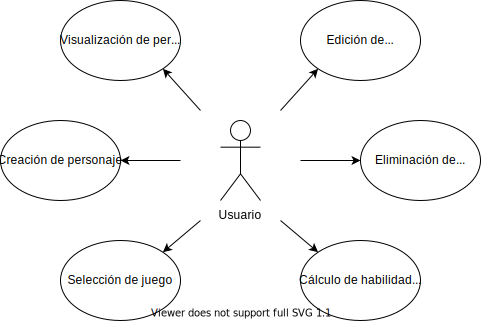
\includegraphics[scale=0.7]{Documentation-Scheme/Desarrollo/Análisis-Sistema/Modelo-Casos-Uso.pdf}
    \caption{Diagrama de Casos de Uso del sistema}
    \label{Caso_uso_sistema}    
\end{figure}

Como en la mayoría de casos de uso es necesario conocer el juego que se va a utilizar, se va a considerar que en los casos 
que no estén directamente relacionados con la gestión de juegos, el primer paso es \textit{Seleccionar juego}, para simplificar 
los diagramas y facilitar su comprensión.

\subsection{Gestión de juegos}

\begin{figure}[H]
    \centering
    \includegraphics[scale=0.7]{Documentation-Scheme/Desarrollo/Análisis-Sistema/Caso_Uso_Juegos.pdf}
    \caption{Diagrama de Casos de Uso: Gestión de juegos}
    \label{Diagrama_gestión_juegos}    
\end{figure}


\subsubsection{Caso de uso: Añadir juego} 
\begin{itemize}
    \item \textbf{Descripción}: El usuario añade un juego o una versión de un juego a la aplicación.
    \item \textbf{Precondiciones}: El usuario debe disponer del fichero de información del juego en el 
    dispositivo que contiene la aplicación.
    \item \textbf{Postcondiciones}: La aplicación tiene acceso a un nuevo juego.
\end{itemize}

\paragraph{\textit{Identificación de escenarios}}
\subparagraph{Escenario principal}
\begin{enumerate}
    \item El usuario desea introducir un nuevo juego en la aplicación.
    \item El usuario pulsa el botón de \textit{Añadir juego}.
    \item El usuario selecciona la opción \textit{Juego nuevo}.
    \item El usuario introduce el nombre del juego.
    \item El usuario indica el fichero de información del juego.
    \item El usuario pulsa el botón de \textit{Aceptar}.
    \item El sistema crea la estructura de carpetas para el nuevo juego.
    \item El sistema copia el fichero en su nueva ubicación, de manera que ya está listo 
    para su uso en el sistema.
\end{enumerate}

\subparagraph{Escenario alternativo: Añadir nueva versión de un juego ya existente}
\begin{enumerate}
    \item El usuario desea introducir un nuevo juego en la aplicación.
    \item El usuario pulsa el botón de \textit{Añadir juego}.
    \item El usuario selecciona la opción \textit{Actualizar juego}.
    \item El usuario indica el directorio en el que debe ubicarse el juego que desea incluir.
    \item El usuario indica el fichero de información del juego.
    \item El usuario pulsa el botón de \textit{Aceptar}.
    \item El sistema copia el fichero en su nueva ubicación, de manera que ya está listo 
    para su uso en el sistema.
\end{enumerate}

\subsubsection{Caso de uso: Seleccionar juego}
\begin{itemize}
    \item \textbf{Descripción}: El usuario elige un juego disponible en la aplicación.
    \item \textbf{Precondiciones}: El usuario debe disponer de algún juego en la aplicación.
    \item \textbf{Postcondiciones}: La aplicación toma el juego y la versión indicados
    como juego y versión activos hasta que se realice una nueva selección.
\end{itemize}

\paragraph{\textit{Identificación de escenarios}}
\subparagraph{Escenario principal}
\begin{enumerate}
    \item El usuario desea seleccionar un juego de la aplicación.
    \item El usuario pulsa el botón de \textit{Seleccionar juego}.
    \item El sistema muestra un listado con los juegos disponibles.
    \item El usuario selecciona una de las opciones mostradas.
    \item El sistema muestra todas las versiones disponibles del juego seleccionado.
    \item El usuario selecciona una de las opciones mostradas.
    \item El usuario pulsa el botón de \textit{Aceptar}.
    \item El sistema crea la estructura de carpetas para el nuevo juego.
    \item El sistema copia el fichero en su nueva ubicación, de manera que ya está listo 
    para su uso en el sistema.
\end{enumerate}

\subsubsection{Caso de uso: Eliminar juego}
\begin{itemize}
    \item \textbf{Descripción}: El usuario elimina un juego disponible de la aplicación.
    \item \textbf{Precondiciones}: El usuario debe disponer de algún juego en la aplicación.
    \item \textbf{Postcondiciones}: La aplicación elimina toda la información relacionada 
    con el juego en cuestión.
\end{itemize}

\newpage
\paragraph{\textit{Identificación de escenarios}}
\subparagraph{Escenario principal}
\begin{enumerate}
    \item El usuario desea eliminar un juego de la aplicación.
    \item El usuario pulsa el botón de \textit{Eliminar juego}.
    \item El usuario selecciona la opción de \textit{Eliminar juego completo}.
    \item El sistema muestra un listado con los juegos disponibles.
    \item El usuario selecciona una de las opciones mostradas.
    \item El sistema realiza una pregunta de confirmación.
    \item El usuario pulsa la opción \textit{Eliminar}.
    \item El sistema elimina todos los elementos relacionados con el juego seleccionado.
\end{enumerate}

\subparagraph{Escenario alternativo: Eliminar una versión de un juego sin eliminar el juego completo}
\begin{enumerate}
    \item El usuario desea eliminar un juego de la aplicación.
    \item El usuario pulsa el botón de \textit{Eliminar juego}.
    \item El usuario \textbf{no} selecciona la opción de \textit{Eliminar juego completo}.
    \item El sistema muestra un listado con los juegos disponibles.
    \item El usuario selecciona una de las opciones mostradas.
    \item El sistema muestra todas las versiones disponibles del juego seleccionado.
    \item El usuario selecciona una de las opciones mostradas.
    \item El usuario pulsa el botón \textit{Aceptar}.
    \item El sistema realiza una pregunta de confirmación.
    \item El usuario pulsa la opción \textit{Eliminar}.
    \item El sistema elimina la versión indicada del juego seleccionado.
\end{enumerate}

\newpage
\subsection{Gestión de personajes}
\begin{figure}[H]
    \centering
    \includegraphics[scale=0.7]{Documentation-Scheme/Desarrollo/Análisis-Sistema/Caso_Uso_Personajes.pdf}
    \caption{Diagrama de Casos de Uso: Gestión de personajes}
    \label{Diagrama_gestión_personajes}    
\end{figure}

\subsubsection{Caso de uso: Crear personaje}
\begin{itemize}
    \item \textbf{Descripción}: El usuario crea un personaje siguiendo las normas del juego y la versión activos.
    \item \textbf{Precondiciones}: El usuario debe haber seleccionado el juego deseado previamente.
    \item \textbf{Postcondiciones}: La aplicación genera un fichero con la información del personaje 
    y lo almacena en la carpeta de personajes correspondiente al juego activo.
\end{itemize}

\paragraph{\textit{Identificación de escenarios}}
\subparagraph{Escenario principal}
\begin{enumerate}
    \item El usuario desea crear un personaje del juego activo en la aplicación.
    \item El usuario pulsa el botón de \textit{Crear personaje}.
    \item El usuario introduce el nombre del personaje.
    \item El sistema muestra las diversas etapas de creación del personaje correspondiente del juego, presentadas 
    a modo de carrusel, de manera que permite al usuario avanzar y retroceder de etapa según lo necesite.
    \item El usuario configura el personaje a su medida.
    \item El usuario presiona el botón \textit{Finalizar} una vez ha terminado de configurar el personaje.
    \item El sistema genera el fichero del personaje y lo almacena en la carpeta de personajes del juego correspondiente.
\end{enumerate}

\subsubsection{Caso de uso: Visualizar personaje}
\begin{itemize}
    \item \textbf{Descripción}: El usuario visualiza un personaje del juego activos.
    \item \textbf{Precondiciones}: El personaje debe haber sido creado previamente.
    \item \textbf{Postcondiciones}: La aplicación muestra la información del personaje.
\end{itemize}

\paragraph{\textit{Identificación de escenarios}}
\subparagraph{Escenario principal}
\begin{enumerate}
    \item El usuario desea visualizar la información de un personaje del juego activo en la aplicación.
    \item El usuario pulsa el botón de \textit{Visualizar personaje}.
    \item El sistema muestra el listado de personajes del juego activo.
    \item El usuario selecciona una de las opciones mostradas.
    \item El sistema muestra la información del usuario, separada por etapas a modo de carrusel, de manera 
    que permite al usuario navegar entre etapas según lo necesite.
\end{enumerate}

\subparagraph{Escenario alternativo: Editar información del personaje}
\begin{enumerate}
    \item Este escenario se describe en el caso de uso \textit{Editar personaje}.
\end{enumerate}

\subparagraph{Escenario alternativo: Eliminar personaje}
\begin{enumerate}
    \item Este escenario se describe en el caso de uso \textit{Eliminar personaje}.
\end{enumerate}

\subsubsection{Caso de uso: Editar personaje}
\begin{itemize}
    \item \textbf{Descripción}: El usuario modifica información de un personaje del juego activo.
    \item \textbf{Precondiciones}: El personaje debe haber sido creado previamente.
    \item \textbf{Postcondiciones}: La aplicación sobreescribe la información del personaje.
\end{itemize}

\newpage
\paragraph{\textit{Identificación de escenarios}}
\subparagraph{Escenario principal}
\begin{enumerate}
    \item El usuario desea visualizar la información de un personaje del juego activo en la aplicación.
    \item El usuario pulsa el botón de \textit{Visualizar personaje}.
    \item El sistema muestra el listado de personajes del juego activo.
    \item El usuario selecciona una de las opciones mostradas.
    \item El sistema muestra la información del usuario, separada por etapas a modo de carrusel, de manera 
    que permite al usuario navegar entre etapas según lo necesite.
    \item El usuario pulsa el botón de \textit{Editar información de etapa}.
    \item El sistema muestra la vista de edición de la etapa en cuestión.
    \item El usuario altera en parte o en su totalidad el contenido de la vista.
    \item El usuario pulsa el botón \textit{Guardar cambios}
    \item El sistema realiza una pregunta de seguridad.
    \item El usuario pulsa el botón \textit{Guardar}.
    \item El sistema sobreescribe el fichero del personaje con los nuevos valores.
\end{enumerate}

\subsubsection{Caso de uso: Eliminar personaje}
\begin{itemize}
    \item \textbf{Descripción}: El usuario elimina un personaje del juego activo.
    \item \textbf{Precondiciones}: El personaje debe haber sido creado previamente.
    \item \textbf{Postcondiciones}: La aplicación sobreescribe la información del personaje.
\end{itemize}

\paragraph{\textit{Identificación de escenarios}}
\subparagraph{Escenario principal}
\begin{enumerate}
    \item El usuario desea visualizar la información de un personaje del juego activo en la aplicación.
    \item El usuario pulsa el botón de \textit{Visualizar personaje}.
    \item El sistema muestra el listado de personajes del juego activo.
    \item El usuario selecciona una de las opciones mostradas.
    \item El sistema muestra la información del usuario, separada por etapas a modo de carrusel, de manera 
    que permite al usuario navegar entre etapas según lo necesite.
    \item El usuario pulsa el botón de \textit{Eliminar personaje}.
    \item El sistema realiza una pregunta de seguridad.
    \item El usuario pulsa el botón \textit{Eliminar}.
    \item El sistema elimina el fichero del personaje.
\end{enumerate}

\subsection{Gestión de habilidades}
\begin{figure}[H]
    \centering
    \includegraphics[scale=0.7]{Documentation-Scheme/Desarrollo/Análisis-Sistema/Caso_Uso_Habilidades.pdf}
    \caption{Diagrama de Casos de Uso: Gestión de habilidades}
    \label{Diagrama_gestión_habilidades}    
\end{figure}

\subsubsection{Caso de uso: Calcular habilidad}
\begin{itemize}
    \item \textbf{Descripción}: El usuario conocer el resultado de una habilidad aplicando los modificadores 
    correspondientes al resultado del lanzamiento de dados.
    \item \textbf{Precondiciones}: El personaje debe haber sido creado previamente.
    \item \textbf{Postcondiciones}: La aplicación calcula el valor final de la habilidad aplicando los 
    modificadores almacenados en el fichero del personaje.
\end{itemize}

\paragraph{\textit{Identificación de escenarios}}
\subparagraph{Escenario principal}
\begin{enumerate}
    \item El usuario desea calcular el resultado de una habilidad de un personaje.
    \item El usuario pulsa el botón de \textit{Calcular habilidad de personaje}.
    \item El sistema muestra la pantalla de cálculo de habilidades.
    \item El usuario pulsa el botón de \textit{Seleccionar personaje}.
    \item El sistema muestra el listado de personajes del juego activo.
    \item El usuario selecciona una de las opciones mostradas.
    \item El usuario pulsa el botón de \textit{Seleccionar habilidad}.
    \item El sistema muestra un listado con las habilidades disponibles del personaje.
    \item El usuario selecciona una de las opciones mostradas.
    \item El usuario introduce el valor del lanzamiento de dados.
    \item El usuario pulsa el botón de \textit{Calcular}.
    \item El sistema devuelve el resultado del cálculo.
\end{enumerate}


% Import Section %
% ARPEGOS:  Automatized Roleplaying-game Profile Extensible Generator Ontology based System %
% Author : Alejandro Muñoz Del Álamo %
% Copyright 2019 %

% Section 4.4: Modelo de Interfaz de Usuario %
\section{Modelo de Interfaz de Usuario}
En esta sección se trata la interacción entre el sistema y el usuario a través de las diferentes vistas 
de las que dispone el sistema.

\subsection{Pantalla de inicio}
La pantalla de inicio de la aplicación se muestra cuando la aplicación se inicia. En ella se 
muestran los diferentes juegos actualmente disponibles para la aplicación.
Dispone de dos iconos interactivos en la esquina superior derecha de la pantalla, para añadir o eliminar 
juegos en la aplicación, y un menú contextual, que se puede activar pulsando sobre el icono dispuesto 
en la esquina superior izquierda de la pantalla. Esta vista se puede apreciar en la figura \ref*{PantallaInicio}.
\newpage

\begin{figure}[H]
    \centering
    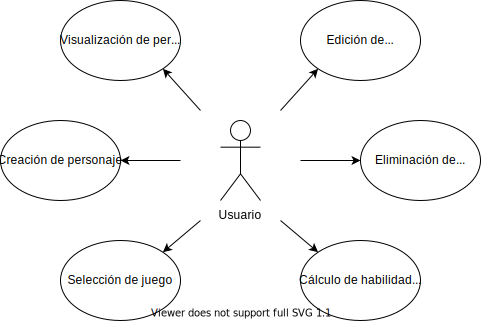
\includegraphics[scale=0.7]{Documentation-Scheme/Desarrollo/Análisis-Sistema/Modelo-Casos-Uso.pdf}
    \caption{Pantalla de inicio}
    \label{PantallaInicio}    
\end{figure}

En el caso de que el usuario desee eliminar uno o varios de los juegos existentes, al pulsar sobre el 
icono de la papelera, surgirá un aviso indicando que está activado el modo de eliminación, de manera que 
al seleccionar un elemento, en vez de acceder a su contenido, lo estará seleccionando para eliminarlo, tal 
y como se muestra en la figura \ref*{ModoEliminacion}. Al seleccionar un juego para eliminarlo, 
la aplicación realizará una pregunta de seguridad, ya que una vez eliminado el juego, no será posible 
recuperarlo (Figura \ref{PreguntaSeguridad}).

\begin{figure}[H]
    \centering
    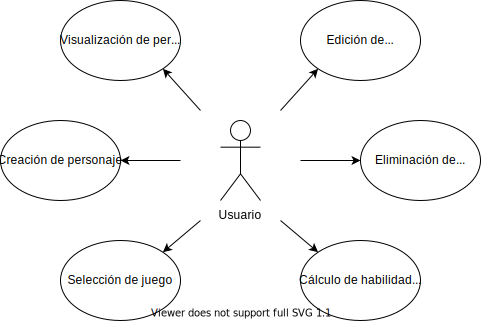
\includegraphics[scale=0.7]{Documentation-Scheme/Desarrollo/Análisis-Sistema/Modelo-Casos-Uso.pdf}
    \caption{Modo de eliminación}
    \label{ModoEliminacion}    
\end{figure}

\begin{figure}[H]
    \centering
    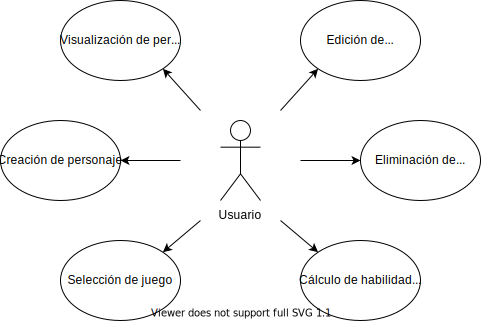
\includegraphics[scale=0.7]{Documentation-Scheme/Desarrollo/Análisis-Sistema/Modelo-Casos-Uso.pdf}
    \caption{Pregunta de seguridad}
    \label{PreguntaSeguridad}    
\end{figure}

\subsection{Pantalla de adición de juego}
A esta vista se puede acceder al pulsar sobre el icono de adición en la esquina superior derecha 
de las pantallas de inicio, y de selección de versión. Esta vista dispone de un icono de flecha en la esquina superior 
izquierda de la pantalla en caso de que se desee volver a la vista previa. En el centro de la pantalla se pueden apreciar 
una caja de texto y tres botones, llamados \textit{Comprobar juego}, \textit{Seleccionar fichero} y \textit{Añadir fichero} 
(figura \ref*{AnadirJuego}). 

\begin{figure}[H]
    \centering
    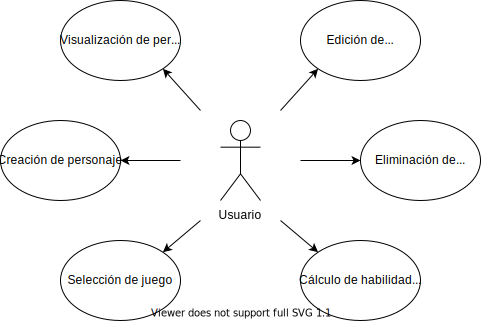
\includegraphics[scale=0.7]{Documentation-Scheme/Desarrollo/Análisis-Sistema/Modelo-Casos-Uso.pdf}
    \caption{Pregunta de seguridad}
    \label{AnadirJuego}    
\end{figure}

En primer lugar, aparece una caja de texto, en la que podemos introducir el nombre del juego que queremos añadir.
A continuación se encuentra el botón \textit{Comprobar juego}, el cual creará la estructura del juego indicado en caso 
de no existir (figura \ref*{ComprobarJuego}). En caso contrario, indicará que dicho juego ya existe. 

\begin{figure}[H]
    \centering
    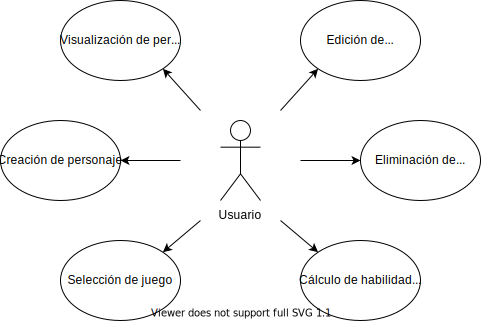
\includegraphics[scale=0.7]{Documentation-Scheme/Desarrollo/Análisis-Sistema/Modelo-Casos-Uso.pdf}
    \caption{Pregunta de seguridad}
    \label{ComprobarJuego}    
\end{figure}

Seguidamente está dispuesto el 
botón \textit{Seleccionar fichero}, que permite al usuario indicar el fichero en el que se encuentra la información del juego, 
haciendo uso del sistema de ficheros del dispositivo (figura \ref*{SeleccionarFichero1}). Una vez seleccionado, el sistema mostrará por pantalla un aviso indicando 
cuál es el fichero seleccionado (figura \ref*{SeleccionarFichero2}). 

\begin{figure}[H]
    \centering
    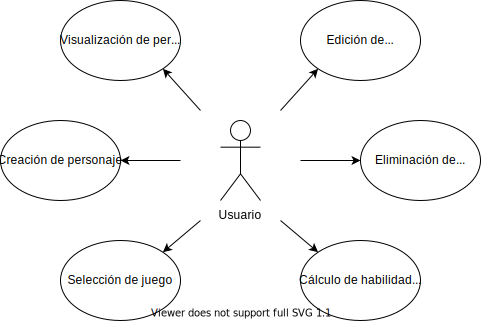
\includegraphics[scale=0.7]{Documentation-Scheme/Desarrollo/Análisis-Sistema/Modelo-Casos-Uso.pdf}
    \caption{Pregunta de seguridad}
    \label{SeleccionarFichero1}    
\end{figure}

\begin{figure}[H]
    \centering
    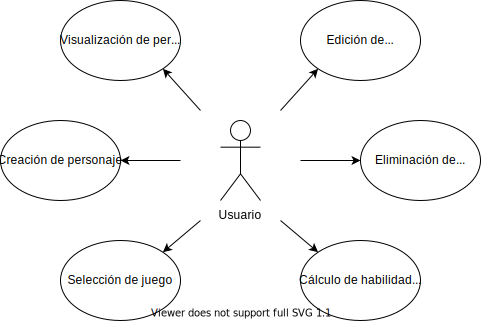
\includegraphics[scale=0.7]{Documentation-Scheme/Desarrollo/Análisis-Sistema/Modelo-Casos-Uso.pdf}
    \caption{Pregunta de seguridad}
    \label{SeleccionarFichero2}    
\end{figure}

En último lugar está el botón \textit{Añadir fichero}, que introduce el fichero previamente 
seleccionado en la carpeta del juego indicado en la caja de texto, y muestra un aviso por pantalla indicando si 
el fichero se ha añadido exitosamente (figura \ref*{AnadirFichero}). 

\begin{figure}[H]
    \centering
    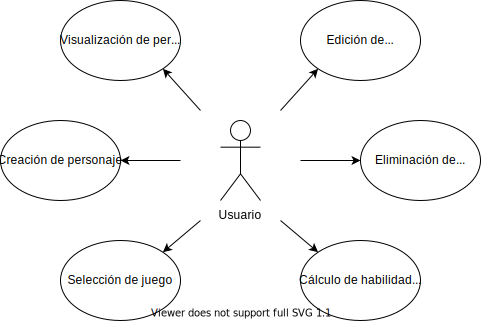
\includegraphics[scale=0.7]{Documentation-Scheme/Desarrollo/Análisis-Sistema/Modelo-Casos-Uso.pdf}
    \caption{Pregunta de seguridad}
    \label{AnadirFichero}    
\end{figure}

\subsection{Menú contextual}
El menú contextual consiste en una vista oculta en la aplicación que se despliega al pulsar un icono de 
tres barras horizontales, ubicado en la esquina superior izquierda de la pantalla (figura \ref*{MenuContextualOculto}).

\begin{figure}[H]
    \centering
    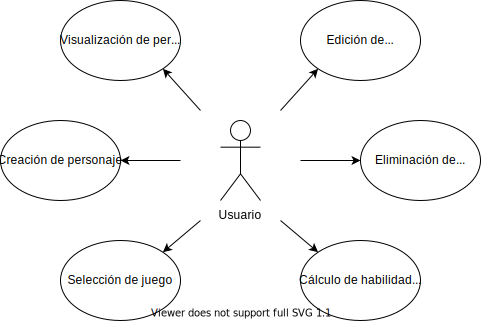
\includegraphics[scale=0.7]{Documentation-Scheme/Desarrollo/Análisis-Sistema/Modelo-Casos-Uso.pdf}
    \caption{Pantalla con menú contextual disponible}
    \label{MenuContextualOculto}    
\end{figure}

Al abrir el menú contextual se muestran tres opciones: \textit{Inicio}, \textit{Seleccionar personaje} y 
\textit{Seleccionar tema}. La primera opción hace que la aplicación retroceda a la pantalla de inicio.
La segunda lleva al usuario a la vista de selección de personaje, siempre y cuando el juego esté seleccionado. 
En caso contrario, el sistema lanzará una alerta avisando que no es posible seleccionar personajes mientras no 
se haya escogido un juego previamente (figura \ref*{MenuContextual}). Por último, la tercera opción abre la vista de 
selección de tema.

\begin{figure}[H]
    \centering
    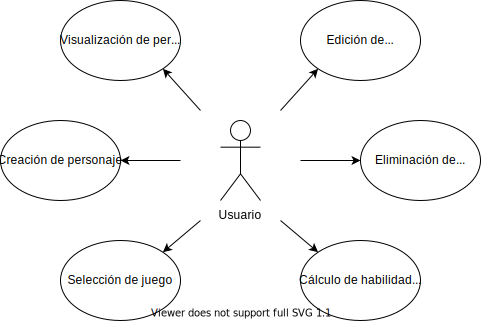
\includegraphics[scale=0.7]{Documentation-Scheme/Desarrollo/Análisis-Sistema/Modelo-Casos-Uso.pdf}
    \caption{Pantalla con menú contextual disponible}
    \label{MenuContextual}    
\end{figure}

\subsection{Pantalla de selección de tema}
Esta vista sólo es accesible desde la opción \textit{Seleccionar tema} del menú contextual.
En ella se muestran diversas opciones de temas de fondo, y un color, referente al color base del tema cuyo nombre acompaña.
Hay siete temas de colores disponibles: 
\begin{itemize}
    \item \textit{Noche} (figura \ref*{Noche})
    \item \textit{Día} (figura \ref*{Dia})
    \item \textit{Bosque} (figura \ref*{Bosque})
    \item \textit{Desierto} (figura \ref*{Desierto})
    \item \textit{Tundra} (figura \ref*{Tundra})
    \item \textit{Valle} (figura \ref*{Valle})
    \item \textit{Océano} (figura \ref*{Oceano})
\end{itemize}

\begin{figure}[H]
    \centering
    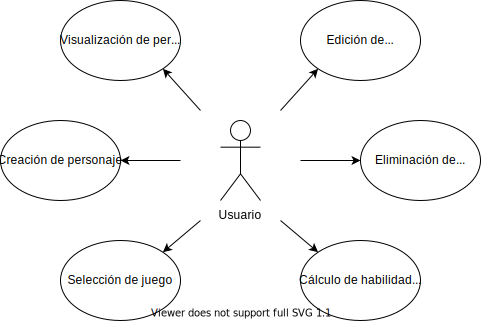
\includegraphics[scale=0.7]{Documentation-Scheme/Desarrollo/Análisis-Sistema/Modelo-Casos-Uso.pdf}
    \caption{Tema \textit{Noche}}
    \label{Noche}    
\end{figure}
\begin{figure}[H]
    \centering
    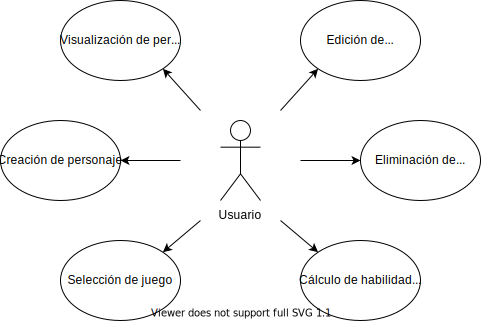
\includegraphics[scale=0.7]{Documentation-Scheme/Desarrollo/Análisis-Sistema/Modelo-Casos-Uso.pdf}
    \caption{Tema \textit{Día}}
    \label{Dia}    
\end{figure}
\begin{figure}[H]
    \centering
    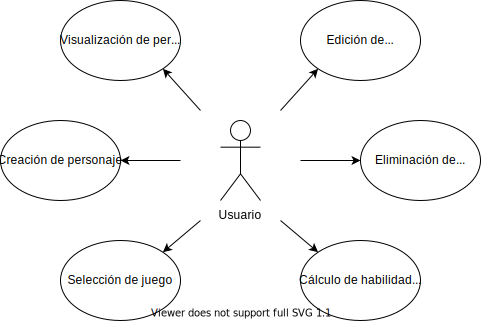
\includegraphics[scale=0.7]{Documentation-Scheme/Desarrollo/Análisis-Sistema/Modelo-Casos-Uso.pdf}
    \caption{Tema \textit{Bosque}}
    \label{Bosque}    
\end{figure}
\begin{figure}[H]
    \centering
    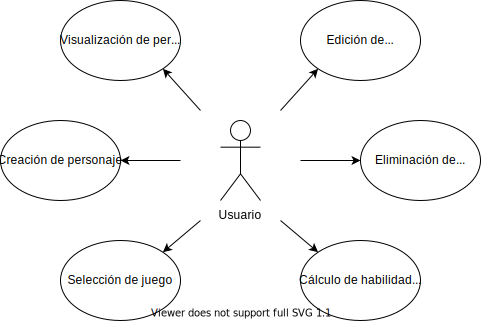
\includegraphics[scale=0.7]{Documentation-Scheme/Desarrollo/Análisis-Sistema/Modelo-Casos-Uso.pdf}
    \caption{Tema \textit{Desierto}}
    \label{Desierto}    
\end{figure}
\begin{figure}[H]
    \centering
    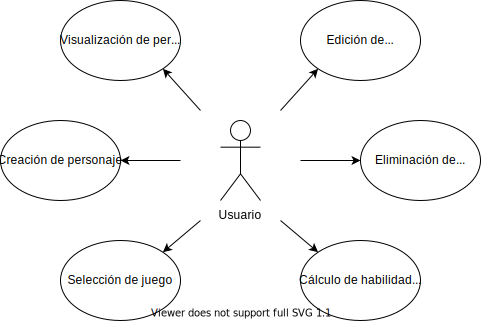
\includegraphics[scale=0.7]{Documentation-Scheme/Desarrollo/Análisis-Sistema/Modelo-Casos-Uso.pdf}
    \caption{Tema \textit{Tundra}}
    \label{Tundra}    
\end{figure}
\begin{figure}[H]
    \centering
    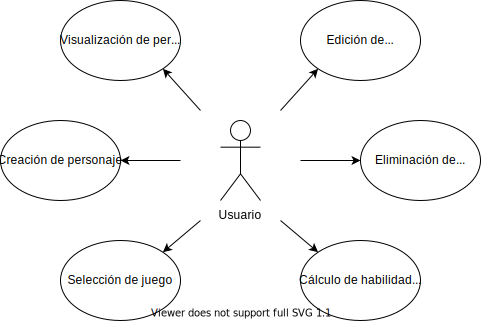
\includegraphics[scale=0.7]{Documentation-Scheme/Desarrollo/Análisis-Sistema/Modelo-Casos-Uso.pdf}
    \caption{Tema \textit{Valle}}
    \label{Valle}    
\end{figure}
\begin{figure}[H]
    \centering
    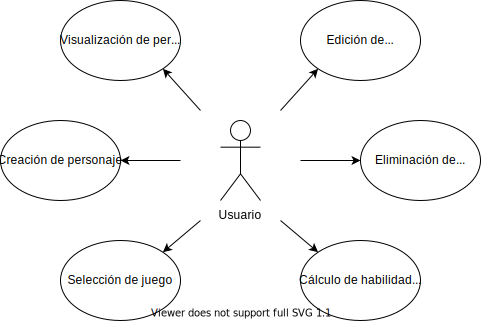
\includegraphics[scale=0.7]{Documentation-Scheme/Desarrollo/Análisis-Sistema/Modelo-Casos-Uso.pdf}
    \caption{Tema \textit{Océano}}
    \label{Oceano}    
\end{figure}

\subsection{Pantalla de selección de versión}
La pantalla de selección de versión se muestra al seleccionar un juego en la pantalla de inicio.
Tiene la misma estructura visual que la pantalla de inicio, pero en este caso se listan las diferentes versiones 
del juego disponibles para la aplicación (figura \ref*{SeleccionVersion}).

\begin{figure}[H]
    \centering
    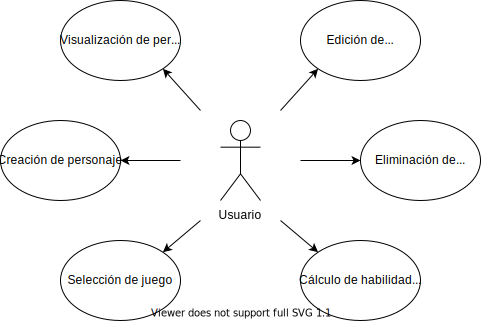
\includegraphics[scale=0.7]{Documentation-Scheme/Desarrollo/Análisis-Sistema/Modelo-Casos-Uso.pdf}
    \caption{Pantalla de selección de versión}
    \label{SeleccionVersion}    
\end{figure}

\subsection{Pantalla de selección de personaje}
Una vez seleccionada la versión del juego a la que se desea acceder, aparece la vista de selección de personaje.
Al igual que la pantalla de selección de versión, la estructura es idéntica a la pantalla de inicio, aunque presenta 
algunas diferencias en funcionalidad. En caso de pulsar el icono de adición de la esquina superior derecha de la pantalla, 
el sistema mostrará una ventana emergente para introducir un nombre, y poder comenzar el proceso de creación de personajes 
(figura \ref*{NombrePersonajeNuevo}).

\begin{figure}[H]
    \centering
    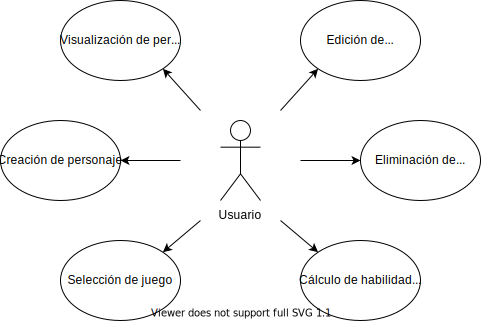
\includegraphics[scale=0.7]{Documentation-Scheme/Desarrollo/Análisis-Sistema/Modelo-Casos-Uso.pdf}
    \caption{Pantalla de selección de personaje}
    \label{NombrePersonajeNuevo}    
\end{figure}

\subsection{Pantallas de creación de personaje}
El proceso de creación de personajes está formado por un conjunto de vistas, que se adaptan a las diferentes etapas del 
proceso en función del tipo de entrada que requieran. Además, algunas de estas disponen de un sistema de control de puntos 
para que el usuario tenga a su disposición el estado actual de puntos de los que dispone para gastar en el proceso.
A continuación se desarrollarán brevemente cada una de ellas.

\subsubsection{Pantalla de selección única}
La vista de selección única forma parte del proceso de creación de personajes. En la parte superior de la 
pantalla se pueden observar el icono de flecha para retroceder a la vista previa y el nombre de la etapa actual.
En el centro de la pantalla se muestran las diversas opciones que se pueden escoger, estructuradas de la siguiente forma:
\begin{itemize}
    \item Un círculo de selección, que indica el elemento seleccionado actualmente.
    \item El nombre del elemento seleccionado
    \item En caso de que el elemento disponga de una descripción, se muestra un icono de información con forma de libro.
\end{itemize}
Esto se puede observar en la figura \ref*{SeleccionUnica}. El sistema no permitirá al usuario avanzar en el proceso de creación 
hasta que haya optado por una de las opciones disponibles. Una vez haya realizado la selección aparecerá un botón \textit{Siguiente}
flotante, para continuar con el proceso, tal y como se enseña en la figura \ref*{Siguiente}.

\begin{figure}[H]
    \centering
    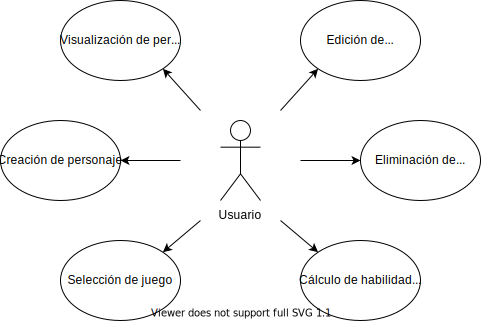
\includegraphics[scale=0.7]{Documentation-Scheme/Desarrollo/Análisis-Sistema/Modelo-Casos-Uso.pdf}
    \caption{Pantalla de selección única}
    \label{SeleccionUnica}    
\end{figure}

\begin{figure}[H]
    \centering
    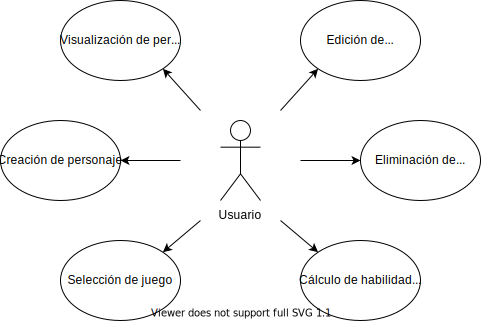
\includegraphics[scale=0.7]{Documentation-Scheme/Desarrollo/Análisis-Sistema/Modelo-Casos-Uso.pdf}
    \caption{Pantalla de selección única con botón \textit{Siguiente} flotante.}
    \label{Siguiente}    
\end{figure}

\subsubsection{Pantalla de selección única con grupos}
La vista de selección única con grupos es similar en funcionalidad a la pantalla de selección única, con una ligera diferencia.
Al acceder a la vista, los elementos que se muestran por pantalla son los diferentes grupos que forman parte de la etapa de creación
(figura \ref*{SeleccionUnicaGrupoCerrado}). Al pulsar sobre uno de los grupos, éste se expande, mostrando todos los elementos 
contenidos en él (figura \ref*{SeleccionUnicaGrupoAbierto}). En caso de intentar abrir varios grupos, sólo quedará expandido 
el último seleccionado, quedando el resto contraídos, para facilitar la navegación por las distintas opciones de la etapa.

\begin{figure}[H]
    \centering
    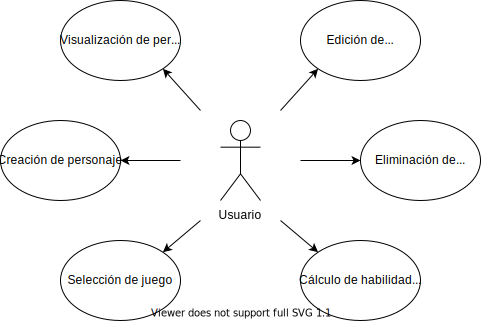
\includegraphics[scale=0.7]{Documentation-Scheme/Desarrollo/Análisis-Sistema/Modelo-Casos-Uso.pdf}
    \caption{Pantalla de selección única}
    \label{SeleccionUnicaGrupoCerrado}    
\end{figure}
\begin{figure}[H]
    \centering
    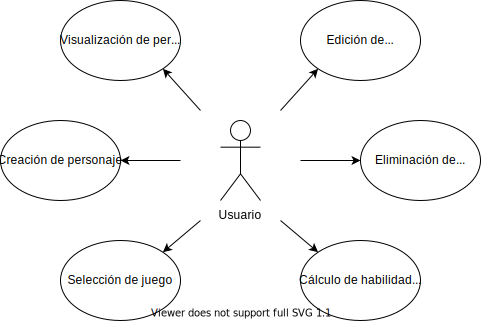
\includegraphics[scale=0.7]{Documentation-Scheme/Desarrollo/Análisis-Sistema/Modelo-Casos-Uso.pdf}
    \caption{Pantalla de selección única}
    \label{SeleccionUnicaGrupoAbierto}    
\end{figure}

\subsubsection{Pantalla de selección múltiple}
La vista de selección múltiple es una semejante a la vista de selección única, con la diferencia de que los círculos de selección 
se han sustituido por cajas de selección múltiple (figura \ref*{SeleccionMultiple}).

\begin{figure}[H]
    \centering
    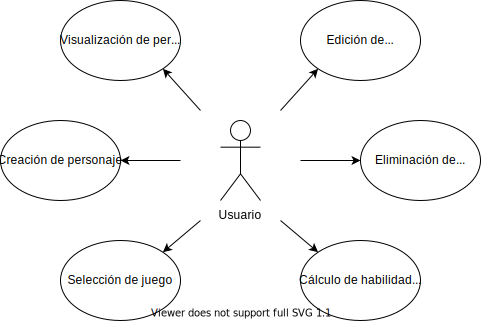
\includegraphics[scale=0.7]{Documentation-Scheme/Desarrollo/Análisis-Sistema/Modelo-Casos-Uso.pdf}
    \caption{Pantalla de selección única}
    \label{SeleccionMultiple}    
\end{figure}

\subsubsection{Pantalla de selección múltiple con grupos}
Esta vista es similar a la pantalla de selección única con grupos, habiendo sustituido los círculos de selección por 
cajas de selección múltiple (figura \ref*{SeleccionMultipleGrupos}).

\begin{figure}[H]
    \centering
    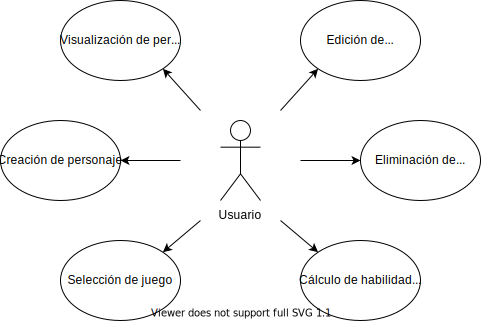
\includegraphics[scale=0.7]{Documentation-Scheme/Desarrollo/Análisis-Sistema/Modelo-Casos-Uso.pdf}
    \caption{Pantalla de selección única}
    \label{SeleccionMultipleGrupos}    
\end{figure}

\subsubsection{Pantalla de gasto de puntos}
La vista de gasto de puntos muestra todos los elementos disponibles de una etapa de creación, y el valor del elemento 
que se desea añadir, acompañado por dos botones (de restar y sumar, respectivamente) para modificar dicho valor 
(figura \ref*{GastoPuntos}).

\begin{figure}[H]
    \centering
    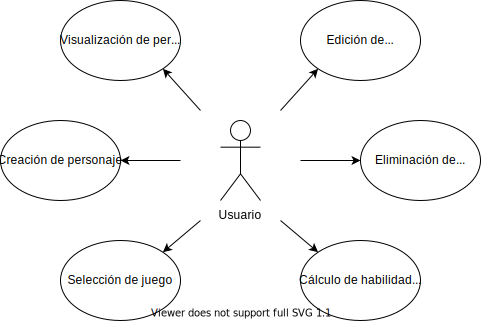
\includegraphics[scale=0.7]{Documentation-Scheme/Desarrollo/Análisis-Sistema/Modelo-Casos-Uso.pdf}
    \caption{Pantalla de gasto de puntos}
    \label{GastoPuntos}    
\end{figure}

\subsubsection{Pantalla de gasto de puntos con grupos}
Esta vista funciona de la misma manera que la pantalla con gasto de puntos, pero incluyendo el trato de grupos del 
que disponen las pantallas de vista única y vista múltiple con grupos (figura \ref*{SeleccionMultipleGrupos}).

\begin{figure}[H]
    \centering
    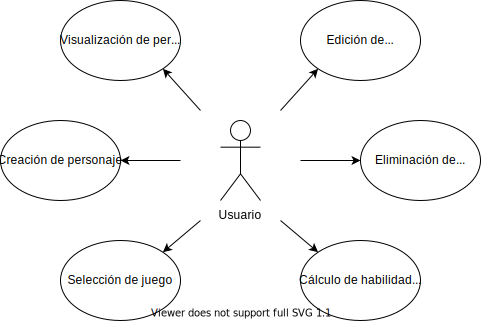
\includegraphics[scale=0.7]{Documentation-Scheme/Desarrollo/Análisis-Sistema/Modelo-Casos-Uso.pdf}
    \caption{Pantalla de gasto de puntos con grupos}
    \label{GastoPuntosGrupos}    
\end{figure}

\subsection{Pantalla de opciones del personaje}
Esta vista es muy sencilla, ya que solo muestra dos botones: uno para visualizar la información del personaje 
(\textit{Visualizar información}), y otro para calcular el valor de las habilidades del personaje (\textit{Calcular habilidad}), 
como se puede ver en la figura \ref*{OpcionesPersonaje}.

\begin{figure}[H]
    \centering
    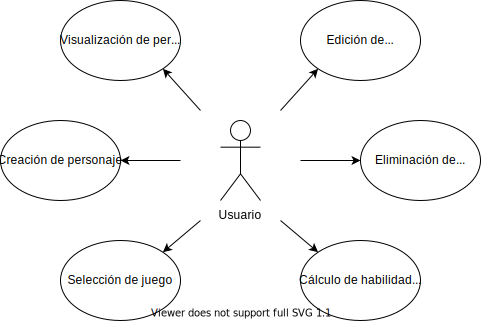
\includegraphics[scale=0.7]{Documentation-Scheme/Desarrollo/Análisis-Sistema/Modelo-Casos-Uso.pdf}
    \caption{Pantalla de opciones del personaje}
    \label{OpcionesPersonaje}    
\end{figure}

\subsection{Pantalla de campos del personaje}
En esta vista se muestran los diferentes campos de información de los que dispone el personaje.
Para visualizar uno de los campos, basta con seleccionarlo. La estructura es similar a la de la 
pantalla de inicio, a excepción de los iconos de la zona superior de la pantalla (figura \ref*{CamposPersonaje}).

\begin{figure}[H]
    \centering
    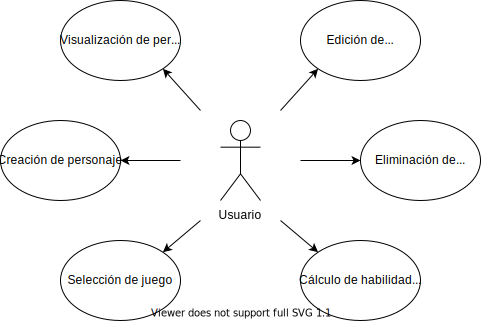
\includegraphics[scale=0.7]{Documentation-Scheme/Desarrollo/Análisis-Sistema/Modelo-Casos-Uso.pdf}
    \caption{Pantalla de campos del personaje}
    \label{CamposPersonaje}    
\end{figure}

\subsection{Pantalla de información del personaje}
Esta vista muestra la información de uno de los campos del personaje, agrupada por secciones, tal y como 
se puede observar en la figura \ref*{InfoPersonaje}.


\begin{figure}[H]
    \centering
    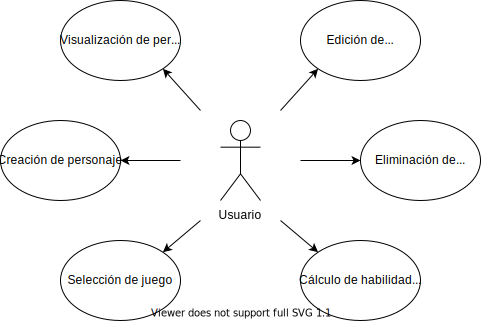
\includegraphics[scale=0.7]{Documentation-Scheme/Desarrollo/Análisis-Sistema/Modelo-Casos-Uso.pdf}
    \caption{Pantalla de información del personaje}
    \label{InfoPersonaje}    
\end{figure}

\subsection{Pantalla de cálculo de habilidad}
Finalmente, la vista de cálculo de habilidad permite seleccionar una habilidad del personaje y 
calcular el resultado total del intento del personaje al realizar dicha habilidad. La vista dispone de varios elementos, 
que se pueden apreciar claramente en la figura \ref*{CalculoHabilidad}.
\begin{itemize}
    \item Un botón de selección de habilidad.
    \item Un recuadro que indica la habilidad seleccionada.
    \item Un cuadro de texto para introducir el valor de una tirada de dados.
    \item Un botón para calcular el resultado de sumar el valor final de la habilidad del personaje al de la tirada.
\end{itemize}

\begin{figure}[H]
    \centering
    \includegraphics[scale=0.7]{Documentation-Scheme/Desarrollo/Análisis-Sistema/Modelo-Casos-Uso.pdf}
    \caption{Pantalla de cálculo de habilidad}
    \label{CalculoHabilidad}    
\end{figure}

\subsection{Pantalla de selección de habilidad}
La vista de selección de habilidad muestra las diferentes habilidades por las que el personaje podría 
realizar un cálculo de habilidad. Para seleccionar una, basta con pulsar el recuadro en el que se encuentra 
el nombre de dicha habilidad (figura \ref*{SeleccionHabilidad}).

\begin{figure}[H]
    \centering
    \includegraphics[scale=0.7]{Documentation-Scheme/Desarrollo/Análisis-Sistema/Modelo-Casos-Uso.pdf}
    \caption{antalla de selección de habilidad}
    \label{SeleccionHabilidad}    
\end{figure}


\blankpage{}

% Import Chapter %
% ARPEGOS:  Automatized Roleplaying-game Profile Extensible Generator Ontology based System %
% Author : Alejandro Muñoz Del Álamo %
% Copyright 2019 %

% Chapter 5: Diseño del Sistema %

\chapter{Diseño del Sistema}
\thispagestyle{chapterpage}

En este capítulo se abordan las diferentes fases de diseño que se 
han realizado durante el desarrollo del proyecto: el diseño de la 
arquitectura del sistema, el diseño de la lógica de negocio de la 
aplicación, y el diseño de la implementación del sistema.

% Import Section %
% ARPEGOS:  Automatized Roleplaying-game Profile Extensible Generator Ontology based System %
% Author : Alejandro Muñoz Del Álamo %
% Copyright 2019 %

% Section 5.2: Diseño de la Lógica de Datos %


% Import Section %
% ARPEGOS:  Automatized Roleplaying-game Profile Extensible Generator Ontology based System %
% Author : Alejandro Muñoz Del Álamo %
% Copyright 2019 %

% Section 5.2: Diseño lógico de Datos %
\section{Diseño Lógico de Datos}
\subsection{Introducción}
En esta sección se va a exponer de forma detallada el proceso de diseño de la ontología que será desarrollada 
para el proyecto. Con este objetivo, se realizará un estudio del diagrama conceptual 
que se muestra en el apartado \ref{Modelo_conceptual}. Este proceso de transformar el esquema del 
modelo conceptual a una estructura lógica que permita almacenar los datos de la aplicación de la 
manera adecuada, se conoce como \textit{diseño lógico}. \medskip

Antes de abordar el proceso, cabe destacar que para poder realizar una ontología que permita comprobar 
que el proyecto puede trabajar con \textit{RPGs} de todo tipo de complejidad, es necesario que el 
juego que se utilice como ejemplo sea lo más completo posible, de manera que juegos de igual o menor   
complejidad puedan ser desarrollados y utilizados asegurando la fiabilidad y completitud de la aplicación. \medskip

Por consiguiente, y tras realizar búsquedas de juegos de rol en base a su complejidad, el equipo de 
desarrollo ha tomado la decisión de utilizar como juego de ejemplo \textit{\textbf{Ánima: Beyond Fantasy}}.
\anima es un juego de rol de mesa que transcurre en un mundo de magia y fantasía, con un sistema
bastante detallado y una complejidad muy elevada, hasta el punto de que hay jugadores que lo evitan 
debido a la larga duración del proceso de creación de personaje, por lo que hace de este juego un caso 
perfecto para demostrar la eficacia de este proyecto.

\subsection{Metodología}
Antes de proceder al desarrollo de la ontología de \anima, se ha considerado fundamental plantear 
que es imposible abordar una fuente de información tan compleja como un \textit{RPG} directamente. En consecuencia, 
el equipo de desarrollo ha procedido a modular el diseño de la ontología, de modo que se aborden los diferentes 
elementos de la ontología por separado, y poco a poco se vayan acoplando hasta que se obtenga el resultado final. \medskip

\subsubsection{Individuos}
Como se ha indicado previamente en el apartado \ref*{Elementos_modelo_conceptual} de la sección \ref*{Modelo_conceptual}, 
un individuo es la \textit{la representacion de un objeto real en el dominio}. Para la elaboración de la ontología de 
\anima, se considerará que un individuo es \textit{la representación de un elemento del dominio, y por tanto, 
tiene una o varias propiedades que lo definen}.

\subsubsection{Clase}
En una ontología, una clase consiste en \textit{un conjunto de individuos que comparten las mismas propiedades y/o 
comportamientos}, tal y como se ha mencionado en el apartado \ref*{Elementos_modelo_conceptual} 
de la sección \ref*{Modelo_conceptual}.

\subsubsection{Propiedades}
La \textit{Real Academia Española} \autocite*{propiedadRAE} define una propiedad como 
\textit{“Atributo o cualidad esencial de alguien o algo”}. Según indica la referencia del 
\textit{OWL Web Ontology Language Reference} \autocite*{Bechhofer2004a}, \textit{OWL} distingue 
dos categorías principales de propiedades:

\begin{itemize}
    \item \textit{\textbf{Datatype properties}}: Las propiedades de tipos de datos conectan individuos con valores de datos.
    \item \textit{\textbf{Object properties}}: Las propiedades de objeto conectan individuos con otros individuos.
\end{itemize}

\subsubsection{Anotaciones}
Como definen Parsia y Kalyanpur \autocite*{Parsia2004}, una anotación es una propiedad que se puede aplicar de manera uniforme a todos los tipos de entidad 
de \textit{OWL}: ontologías, clases, individuos y propiedades. Esta propiedad se considera como un 
comentario, y aunque no pueden definir axiomas, permiten añadir información útil a las entidades pertenecientes 
a cualquier ontología. \medskip

Las anotaciones son un elemento fundamental para el desarrollo de este proyecto, pues posibilitan la introducción de 
información necesaria para algunas entidades de las ontologías, que no pueden o no deben ser indicadas como propiedades 
de las mismas, pues no forman parte de su descripción, sino que aportan información 
imprescindible para el correcto funcionamiento de la aplicación.\medskip

En este proyecto se utilizan diversos tipos de anotaciones, que se podrían separar en dos conjuntos:
\begin{itemize}
    \item \textit{\textbf{Standard annotations}}: Consideramos anotaciones estándar a aquellas que permiten introducir 
    información extra a cualquier entidad de la ontología, incluyendo a esta última también. Son anotaciones que están 
    definidas previamente. Este conjunto esta formado por las siguientes anotaciones:

    \begin{itemize}
        
        \item \textit{rdfs:comment}: Esta anotación se utilizará como descripción de las entidades a las que se vincula, por lo que 
        deberá contener la referencia completa de información del elemento al que hace alusión. El tipo de dato asociado debe ser 
        \textbf{xsd:string}.

        \item \textit{rdfs:IsDefinedBy}: Esta anotación permite indicar qué elemento indica o define el valor 
        de la entidad a la que está asociada. Sólo debe contener el nombre de dicho elemento con el tipo de dato \textbf{xsd:string}.
    \end{itemize}

    \item \textit{\textbf{Stage annotations}}: Las anotaciones de etapa son anotaciones definidas por el equipo de desarrollo 
    para poder aportar la información necesaria para determinar qué entidades se pueden considerar como \textit{etapas de creación}, 
    y de qué manera deben ser procesadas. Toda ontología que pertenezca a este proyecto deberá disponer de ellas adecuadamente para 
    definir las etapas de creación de un personaje. A continuación se indica cuales son:

    \begin{itemize}
        \item \textit{CreationScheme}: Esta anotación describe cuál es el esquema de creación de un personaje. Debe contener 
        de manera ordenada las diversas etapas por las que debe pasar el usuario para crear su personaje. Esta anotación 
        debe ubicarse en cada individuo de la etapa raíz del proceso de creación, utilizando el tipo de dato \textbf{xsd:string}.

        \item \textit{CreationSchemeRoot}: Esta anotación indica qué clase representa la etapa raíz del proceso de creación. 
        Debe estar ubicada en el individuo de la clase \textit{\textbf{ClassDefinition}} correspondiente a la etapa raíz del 
        proceso de creación, y debe tener asociado el valor booleano \textbf{true}.

        \item \textit{GeneralCostDefinedBy}: Esta anotación permite indicar qué elemento define el valor máximo de 
        puntos de una o varias etapas. Debe ser asociada al individuo de la clase \textit{\textbf{ClassDefinition}} correspondiente 
        a la etapa de creación que así lo requiera. Se utiliza de la misma forma que la anotación \textit{rdfs:IsDefinedBy}.

        \item \textit{SubstageOrder}: Esta anotación indica a las etapas que lo requieran, en qué posición se debe mostrar. 
        Normalmente se utiliza en etapas que formen parte de una etapa más general, siendo aplicada al individuo de la clase 
        \textit{\textbf{ClassDefinition}} correspondiente. Su valor debe ser númerico 
        y estar acompañado del tipo de datos \textbf{xsd:unsignedInt}
        
        \item \textit{ValuedListInfo}: Esta anotación debe contener toda la información necesaria para que una etapa de creación 
        que requiera de la vista de introducción de valores realice los cálculos de la manera adecuada. Debe estar asociada 
        al individuo de la clase \textit{\textbf{ClassDefinition}} correspondiente, y debe utilizar el tipo de datos \textbf{xsd:string}.
        
        \item \textit{ViewType}: Esta anotación indica el tipo de vista que debe mostrar la interfaz gráfica de la aplicación 
        cuando se muestre la etapa a la que está vinculada. Debe estar asociada al individuo de la clase 
        \textit{\textbf{ClassDefinition}} correspondiente, y debe indicar el nombre exacto del tipo de vista utilizando
        el tipo de datos \textbf{xsd:string}.
        
    \end{itemize}
\end{itemize}


\subsubsection{Etapas de creación}
Uno de los objetivos del proyecto es que a la hora de crear el personaje, el usuario pueda conocer de forma clara los 
pasos que requiere el juego para crear el personaje de la forma más completa posible. A estos pasos los llamaremos 
\textit{etapas de creación}.\medskip

Para poder definir las etapas de creación de \anima, se han planteado las siguientes preguntas:

\begin{enumerate}
    \item ¿Cuáles son las etapas de creación de personajes del \anima?
    \item ¿Se pueden dividir esas etapas en subetapas más pequeñas?
    \item ¿Cuál debe ser la etapa inicial del proceso de creación?
    \item ¿Son necesarias todas las etapas de creación para cada personaje?
    \item ¿Qué tipo de interacción debe tener el usuario con cada etapa?
\end{enumerate}

La primera respuesta suele encontrarse en los libros de los juegos de rol, ya que es una información 
fundamental para poder crear los personajes. Así sucede en el caso de \anima, de manera que 
echando un ojo rápido al libro, podemos saber que las etapas de creación de un personaje en \anima
son las siguientes: \medskip

\begin{figure}[H]
    \centering
    \includegraphics[scale=0.5]{Documentation-Scheme/Desarrollo/Diseño-Sistema/Etapas_Anima.pdf}
    \caption{Etapas de creación de \textit{Ánima: Beyond Fantasy}}
    \label{Etapas_anima}
\end{figure}

Aunque el proceso aparenta ser rápido y sencillo en un principio, cabe recordar que \anima es conocido 
entre los jugadores de rol por su gran complejidad en la creación de personajes, llegando al punto de frustrar a 
los jugadores debido a la inmensidad de información necesaria para completar el personaje. En consecuencia, se 
ha considerado inviable abordar el proceso de creación de forma directa, y se ha planteado modular el proceso en 
un mayor número de etapas, que sean más sencillas e intuitivas. Así, el equipo de desarrollo considera 
\textbf{preferible un proceso largo de etapas sencillas} a un proceso corto de etapas complejas. \medskip

Después de investigar sobre el juego en profundidad, el equipo de desarrollo ha desglosado las etapas de 
creación de personajes de \anima en subetapas que pueden ser mostradas en una única vista y que 
facilitan una interacción intuitiva por parte de los usuarios, y por consiguiente, 
serán las \textbf{etapas de creación} de nuestra aplicación. El diagrama de flujo resultante se puede 
observar en la figura \ref*{Diagrama_creacion_anima} \footnote[1]{Se adjunta una versión ampliada como anexo 
para poder leer el diagrama adecuadamente.}.\medskip

Durante la investigación sobre el juego se observa que hay diferentes tipos de personajes, definidos por 
reglas y que presentan una lista de propiedades y habilidades a las que pueden tener acceso. En \anima, 
a estos tipos se les conoce como \textit{Categorías}. En consecuencia, la \textit{Categoría} de un personaje 
determinará las etapas de creación del mismo y es por esto que el primer elemento del proceso deberá ser 
la elección de \textit{Categoría}. \medskip

Una vez conocemos el orden y las etapas de creación de un personaje, falta saber cómo puede interactuar el usuario 
con cada etapa, pues cada una de ellas puede requerir un tipo de acción diferente por parte del usuario. Además, 
cada juego dispone de etapas diferentes, lo que hace inviable diseñar una vista para la interacción de cada etapa 
de cada juego. \medskip

La propuesta del equipo de desarrollo para salvar este obstáculo consiste en \textbf{generalizar los tipos de interacción} que pueden 
requerir las etapas de creación de cualquier juego. Esto permite diseñar sólo una vista por cada tipo de interacción, y posteriormente 
vincular cada etapa con el tipo de interacción más adecuado. En el caso de \anima, se han contemplado los siguientes 
tipos de interacción: 

\begin{itemize}
    \item \textit{\textbf{Selección única}}: El usuario sólo necesita elegir una opción de todas las disponibles.
    \item \textit{\textbf{Selección múltiple}}: El usuario puede elegir varias opciones de todas las disponibles. 
    Este caso tiene varias posibilidades:
    \begin{itemize}
        \item \textit{Coste estático}: Todas las opciones tienen el mismo coste, y en caso de estar agrupados, no es necesario 
        realizar gasto alguno de puntos para poder seleccionar elementos de un grupo.
        \item \textit{Coste estático y de grupo}: Todos las opciones tienen el mismo coste, y en caso de estar agrupados, poder 
        optar a seleccionar elementos de un grupo hay que pagar un coste.
        \item \textit{Coste dinámico}: Cada opción tiene un coste diferente.
    \end{itemize}
    \item \textit{\textbf{Introducción de valores}}: El usuario debe introducir valores en los elementos mostrados.
\end{itemize}\medskip

Después de apreciar estos posibles casos, se han revisado otros posibles \textit{RPGs} para comprobar que los tipos de 
interacción previamente indicados son reutilizables para otros juegos, y por tanto, convenientes para el desarrollo del 
presente proyecto. \newpage

\begin{figure}
    \centering
    \includegraphics[scale=0.18]{Documentation-Scheme/Desarrollo/Diseño-Sistema/Proceso_Creación_Anima.pdf}
    \caption{Proceso de Creación de \textit{Ánima: Beyond Fantasy}}
    \label{Diagrama_creacion_anima}
\end{figure}


% Import Section %
% ARPEGOS:  Automatized Roleplaying-game Profile Extensible Generator Ontology based System %
% Author : Alejandro Muñoz Del Álamo %
% Copyright 2019 %

% Section 5.3: Diagrama de clases %
\section{Diseño de Implementación}
Después de realizar el diseño lógico de datos del sistema, el próximo paso es diseñar la estructura de clases del proyecto.
Esta estructura está compuesta por las diversas clases que se consideran necesarias para el funcionamiento de cualquier sistema 
orientado a objetos, y se puede representar mediante un \textit{diagrama de clases}, que muestra las clases de un sistema
con sus atributos y operaciones, y las relaciones entre éstas. A continuación se muestra el diagrama de clases del proyecto en 
la figura \ref*{DiagramaClases}.\medskip

\begin{figure}[H]
    \centering
    \includegraphics[scale=0.2]{Documentation-Scheme/Desarrollo/Diseño-Sistema/DiagramaClases.pdf}
    \caption{Diagrama de clases de \textit{ARPEGOS}}
    \label{DiagramaClases}
\end{figure}

Como se puede apreciar en el diagrama, algunas clases tienen una relación del tipo \textit{CSharp Partial}. 
Esta relación es una funcionalidad del lenguaje \textit{C\#} que permite implementar una misma clase en 
varios ficheros, lo que permite distribuir los atributos y métodos de una clase entre ellos para facilitar 
la legibilidad y mantenibilidad del código. \newpage Éstas clases parciales se pueden reconocer por contener el nombre 
de la clase con la que están relacionadas, seguidas de un punto y la primera palabra de los métodos que contienen.

\subsection{App}
Esta clase representa la aplicación en su conjunto. Contiene como atributo una instancia de la 
clase \textit{DependencyHelper}.

\subsection{DependencyHelper}
El \textit{DependencyHelper} contiene el contexto de la aplicación y los servicios y modelos de vista 
que muestran algún tipo de dependencia en el proyecto.

\subsection{Context}
La clase \textit{Context} dispone de varios elementos que pueden variar en base al funcionamiento de la 
aplicación. Estos elementos son: 
\begin{itemize}
    \item La ontología del juego actualmente seleccionado, de tipo \textit{GameOntologyService}.
    \item La ontología del personaje actualmente seleccionado, instancia de la clase \textit{CharacterOntologyService}.
    \item El servicio de temas de fondo, objeto de la clase \textit{ThemeHelper}.
    \item El servicio de pantallas de diálogo, de tipo \textit{DialogService};
    \item La vista principal de la aplicación, instancia de la clase \textit{MainView}.
\end{itemize}

\subsection{OntologyService}
El servicio \textit{OntologyService} modela cualquier ontología presente en el sistema del proyecto.

\subsection{GameOntologyService}
Esta clase describe la ontología de cualquier juego disponible en la aplicación, y como tal, 
hereda los atributos y métodos de la clase \textit{OntologyService}, sin añadir ninguna propiedad 
o función aparte de las ya heredadas. 

\subsection{CharacterOntologyService}
Esta clase, que es la más compleja del proyecto, dispone de todos los métodos necesarios para 
poder generar, modificar, actualizar y eliminar personajes de cualquier juego disponible en la aplicación. 

\subsection{ThemeHelper}
El servicio \textit{ThemeHelper} es aquel que dispone el tema de colores y fondo que se muestra 
en pantalla durante la ejecución de la aplicación.

\subsection{DialogService}
El servicio de diálogo permite mostrar ventanas emergentes según sean necesitadas durante la ejecución 
de la aplicación.

\subsection{MainView}
Esta clase modela la vista principal del proyecto. Está formada por dos vistas: la vista de detalles, 
que es la que está activa, y la vista maestra, que contiene el menú contextual.

\blankpage{}

% Import Chapter %
% ARPEGOS:  Automatized Roleplaying-game Profile Extensible Generator Ontology based System %
% Author : Alejandro Muñoz Del Álamo %
% Copyright 2019 %

% Chapter 6: Construcción del Sistema %

\chapter{Codificación}
\thispagestyle{chapterpage}

El capítulo de codificación describe el entorno en el que se 
despliega el sistema, y la estructura del código fuente 
del proyecto.

% Import Section %
% ARPEGOS:  Automatized Roleplaying-game Profile Extensible Generator Ontology based System %
% Author : Alejandro Muñoz Del Álamo %
% Copyright 2019 %

% Section 6.1: Entorno de construcción %
\section{Entorno de construcción}
En esta sección se explican de qué herramientas se van a utilizar para la consecución de este proyecto.

\subsection{Framework}
Este proyecto hará uso de \textit{Xamarin}, un \textit{framework} para el desarrollo de aplicaciones multiplataforma, que 
utiliza \textit{C\#} como lenguaje de programación. \textit{Xamarin} posibilita de que dichas aplicaciones 
compartan el código base mediante \textit{Xamarin.Forms}, que permite crear interfaces de usuario en \textit{XAML} con 
código subyacente en \textit{C\#}, las cuales son representadas como controles nativos para cada plataforma.

\subsection{Entorno de desarrollo integrado}
El entorno de desarrollo integrado a utilizar es \textit{Visual Studio}, en su versión gratuita más actualizada hasta el momento
(\textit{Community 2019}). A continuación se muestran algunos de los motivos que impulsan al equipo de desarrollo a optar por este IDE:
\newpage
\begin{itemize}
    \item Soporte oficial de Xamarin para \textit{Visual Studio}
    \item Biblioteca \textit{RDFSharp} disponible mediante el administrador de paquetes \textit{Nuget}.
    \item Disponibilidad de la herramienta \textit{IntelliSense}, que permite una mayor maniobrabilidad con el código.
\end{itemize}

\begin{figure}[H]
    \centering
    \includegraphics[scale=0.2]{Figures/Logo_VisualStudio.png}
    \caption{Logo de \textit{Visual Studio}}
    \label{Logo_VS}
\end{figure}

\subsection{Editor de ontologías}
\label{Editor_ontologias}
Para la construcción de ontologías se ha utilizado el editor 
\protege en su versión \textit{5.5.0}.

\begin{figure}[H]
    \centering
    \begin{minipage}{0.38\textwidth}
        \centering
        \includegraphics[width=0.4\textwidth]{Figures/Logo_Protege.pdf}
        \caption{Logo de \protege}
    \end{minipage}
\end{figure}

\subsection{Control de versiones}
Se conoce como \textit{control de versiones} a la gestión de las modificaciones que se producen en los componentes de un producto, o en 
su configuración. Aunque puede hacerse manualmente, hoy en día existen herramientas que hacen este proceso más sencillo, cómodo y 
seguro. Estas herramientas se conocen como \textit{sistemas de control de versiones (\textbf{VCS})}.\medskip

Para realizar el control de versiones de este proyecto, se hará uso del VCS \textit{Git}. Además se utilizará la 
plataforma de desarrollo colaborativo \textit{GitHub} como repositorio remoto del proyecto. Así, en caso de que 
se corrompa la versión local del proyecto, será posible recuperar la versión más actualizada del proyecto.
\newpage
% Insertar imagen Git & GitHub
\begin{figure}[H]
    \centering
    \begin{minipage}{0.38\textwidth}
        \centering
        \includegraphics[width=0.5\textwidth]{Figures/Logo_Git.png}
        \caption{Logo de \textit{Git}}
    \end{minipage} \hspace{2cm}
    \begin{minipage}{0.38\textwidth}
        \centering
        \includegraphics[width=0.8\textwidth]{Figures/Logo_GitHub.jpg}
        \caption{Logo de \textit{GitHub}}
    \end{minipage}
\end{figure}

\subsection{Memoria}
En lo referente a la elaboración de la memoria, se ha realizado en \LaTeX, utilizando \textit{Visual Studio Code} como editor 
de texto, con la extensión \textit{\LaTeX Workshop}. Esta última requiere disponer de la distribución \textit{MiKTeX}. 

\begin{figure}[H]
    \centering
    \begin{minipage}{0.38\textwidth}
        \centering
        \includegraphics[width=0.3\textwidth]{Figures/Logo_VSCode.png}
        \caption{Logo de \textit{Git}}
    \end{minipage} \hspace{2cm}
    \begin{minipage}{0.38\textwidth}
        \centering
        \includegraphics[width=0.8\textwidth]{Figures/Logo_MikTex.png}
        \caption{Logo de \textit{GitHub}}
    \end{minipage}
\end{figure}

Por otro lado, para el diseño de diagramas se ha hecho uso de la aplicación \textit{Draw.io} en su versión de 
escritorio y el programa \textit{InkScape} para el tratamiento de imágenes.

% Insertar imagen VSCode, Latex, MikTex, Draw.io & InkScape

\begin{figure}[H]
    \centering
    \begin{minipage}{0.38\textwidth}
        \centering
        \includegraphics[width=0.4\textwidth]{Figures/Logo_Draw.png}
        \caption{Logo de \textit{Git}}
    \end{minipage} \hspace{2cm}
    \begin{minipage}{0.38\textwidth}
        \centering
        \includegraphics[width=0.4\textwidth]{Figures/Logo_Inkscape.png}
        \caption{Logo de \textit{GitHub}}
    \end{minipage}
\end{figure}



% Import Section %
% ARPEGOS:  Automatized Roleplaying-game Profile Extensible Generator Ontology based System %
% Author : Alejandro Muñoz Del Álamo %
% Copyright 2019 %

% Section 7.1: Entorno de Pruebas %
\section{Organización del código fuente}
Como se ha comentado en capítulos anteriores de la presente documentación, el proyecto se ha desarrollado en \textit{Visual Studio}, y se ha aplicado el 
patrón de arquitectura \textit{MVVM}. \medskip

Al haber utilizado \textit{Visual Studio}, la aplicación se ha desarrollado en una \textbf{\textit{solución}}, que es un contenedor que contiene 
uno o más proyectos relacionados, junto a información de compilación, la configuración de \textit{Visual Studio} y archivos no asociados 
a un proyecto determinado. Por otro lado, un \textbf{\textit{proyecto}} es el conjunto de ficheros que se compilan en un archivo ejecutable, 
biblioteca o sitio web.

En lo referente a este proyecto, 





\blankpage{}

% Import Chapter %
% ARPEGOS:  Automatized Roleplaying-game Profile Extensible Generator Ontology based System %
% Author : Alejandro Muñoz Del Álamo %
% Copyright 2019 %

% Chapter 7: Pruebas del sistema %

\chapter{Pruebas del Sistema}
\thispagestyle{chapterpage}

% Import Section %
% ARPEGOS:  Automatized Roleplaying-game Profile Extensible Generator Ontology based System %
% Author : Alejandro Muñoz Del Álamo %
% Copyright 2019 %

% Section 7.2: Niveles de Pruebas %


% Import Section %
\input{Documentation_Scheme/Desarrollo/Pruebas_Sistema/Niveles_Pruebas.tex}
\blankpage{}

    \blankpage{}

    % Import Part III
    % ARPEGOS:  Automatized Roleplaying-game Profile Extensible Generator Ontology based System %
% Author : Alejandro Muñoz Del Álamo %
% Copyright 2019 %

% Part 3: Epílogo %

\part{Epílogo}

% Import Chapter %
% ARPEGOS:  Automatized Roleplaying-game Profile Extensible Generator Ontology based System %
% Author : Alejandro Muñoz Del Álamo %
% Copyright 2019 %

% Chapter 8: Manual de Implantación y Explotación %

\chapter{Manual de instalación}
\thispagestyle{chapterpage}

Este capítulo muestra los requisitos que se debe cumplir un dispositivo
para poder ejecutar la aplicación desarrollada, y los procedimientos 
que se deben seguir para su correcta instalación.
% Import Section %
% ARPEGOS:  Automatized Roleplaying-game Profile Extensible Generator Ontology based System %
% Author : Alejandro Muñoz Del Álamo %
% Copyright 2019 %

% Section 8.3: Inventario de componentes %


% Import Section %
% ARPEGOS:  Automatized Roleplaying-game Profile Extensible Generator Ontology based System %
% Author : Alejandro Muñoz Del Álamo %
% Copyright 2019 %

% Section 8.4: Procedimientos de instalación %
\section{Sistema de ficheros}
Esta aplicación dispone de un sistema de ficheros organizado que permite su correcto funcionamiento y 
facilita su legibilidad y mantenibilidad. Se organiza por juegos, de manera que a cada juego le corresponde
un directorio. Dentro de cada directorio de juego, se encuentran dos carpetas:
\begin{itemize}
    \item \textit{gamefiles}: Aquí se almacenan las diferentes ontologías de un mismo juego.
    \item \textit{characters}: Aquí se generan las ontologías que contienen la información de los personajes.
\end{itemize}

Al instalar la aplicación, dispondrá de la ontología del juego \textit{Ánima: Beyond Fantasy}, a modo de 
ejemplo, por lo que debería aparecer la carpeta con el nombre del juego en la ruta \label{Ruta_ficheros}
\textit{\textbf{Almacenamiento interno/Android/data/com.arpegos/files/}}

% Import Section %
\input{Documentation-Scheme/Epílogo/Manual-Instalacion/Procedimientos_Instalación.tex}
\blankpage{}

% Import Chapter %
% ARPEGOS:  Automatized Roleplaying-game Profile Extensible Generator Ontology based System %
% Author : Alejandro Muñoz Del Álamo %
% Copyright 2019 %

% Chapter 9: Manual de Usuario %

\chapter{Manual de usuario}
\thispagestyle{chapterpage}

% Import Section %
% ARPEGOS:  Automatized Roleplaying-game Profile Extensible Generator Ontology based System %
% Author : Alejandro Muñoz Del Álamo %
% Copyright 2019 %

% Chapter 1: Introducción %

\chapter{Introducción}
\thispagestyle{chapterpage}

% Import Section 1.1 %
\input{Documentation_Scheme/Prolegómeno/Introducción/Motivación.tex}

% Import Section 1.2 %
\input{Documentation_Scheme/Prolegómeno/Introducción/Alcance.tex}

% Import Section 1.3 %
\input{Documentation_Scheme/Prolegómeno/Introducción/Glosario.tex}

% Import Section 1.4 %
\input{Documentation_Scheme/Prolegómeno/Introducción/Organización_Documento.tex}

% Import Section %
% ARPEGOS:  Automatized Roleplaying-game Profile Extensible Generator Ontology based System %
% Author : Alejandro Muñoz Del Álamo %
% Copyright 2019 %

% Section 9.2: Características %
\section{Gestión de Juegos}
\subsection{Añadir juego}
Esta función permite al usuario incluir un nuevo juego o una nueva versión de un juego en el 
sistema. Para ello, es necesario que el fichero que contiene la ontología del juego esté 
disponible en el dispositivo móvil.\medskip

\begin{enumerate}
    \item Acceder al menú principal y pulsar la opción \textit{Añadir juego}.
    \item Indicar si se va a incluir un juego nuevo, o una nueva versión de un juego existente.
    \item Introducir el nombre del juego en el que se va a guardar el nuevo fichero. Si no existe, crea las 
    carpetas correspondientes.
    \item Seleccionar el fichero del juego.
    \item Ya solo queda pulsar el botón \textit{Aceptar} para que el programa introduzca el fichero 
    del juego de la manera adecuada para ser reconocido por la aplicación.
\end{enumerate}

\subsection{Seleccionar juego}
Esta función permite elegir uno de los juegos disponibles como referencia para las diversas funciones 
de la aplicación.\medskip

\begin{enumerate}
    \item Acceder al menú principal y pulsar la opción \textit{Seleccionar juego}. Al hacer esto, 
    se mostrará un listado de los diferentes juegos disponibles.
    \item Elegir uno de los juegos disponibles y pulsar el botón \textit{Continuar}. 
    Una vez elegido, se mostrará un listado con las diferentes versiones del juego disponibles.
    \item Elegir una de las versiones disponibles. Una vez hecho, basta con pulsar el botón \textit{Finalizar}.
    Tras esto, el juego tendrá como referencia la versión seleccionada del juego previamente indicado.
\end{enumerate}

\subsection{Eliminar juego}
Esta función permite eliminar un juego o una versión de un juego existente, de manera que sea posible eliminar aquellos que 
no se utilicen. \medskip

\begin{enumerate}
    \item Acceder al menú principal y pulsar la opción \textit{Eliminar juego}.
    \item Indicar si se va a eliminar un juego completo, o sólo una versión del juego.
    \item Al pulsar el botón \textit{Examinar} se mostrará un listado con los juegos disponibles.
    \item Seleccionar uno de los elementos de la lista y pulsar el botón \textit{Aceptar}.
    \begin{itemize}
        \item Si se va a eliminar una versión de un juego, se mostrará otra lista con las versiones 
        del juego seleccionado.
        \item Elegir una de las opciones mostradas y pulsar \textit{Aceptar}.
    \end{itemize}
    \item Se mostrará una pregunta para confirmar la operación. En caso afirmativo, pulsar el botón \textit{Eliminar}.
    En caso contrario, presionar el botón \textit{Cancelar}.
    \item Tras confirmar la operación, se eliminará el juego o la versión correspondiente.
\end{enumerate}


% Import Section %
% ARPEGOS:  Automatized Roleplaying-game Profile Extensible Generator Ontology based System %
% Author : Alejandro Muñoz Del Álamo %
% Copyright 2019 %

% Section 9.2: Características %
\section{Gestión de Personajes}
\subsection{Añadir personaje}
Esta función permite al usuario crear un nuevo personaje siguiendo las bases del juego que esté seleccionado como activo.
En caso de que el proceso quede sin finalizar, habrá que iniciarlo desde cero.\medskip

\begin{enumerate}
    \item Acceder al menú principal y pulsar la opción \textit{Crear personaje}.
    \item Introducir el nombre del personaje. \textbf{Aviso}: \textit{El nombre de personaje debe ser único.}
    \item Seleccionar una de las opciones listadas en la \textit{etapa raíz} del proceso de creación.
    \item Interactuar con la vista que se muestre, según se requiera (seleccionar uno o varios elementos, o 
    introducir valores).
    \item Utilizar los botones con flechas direccionales para avanzar o retroceder de etapa.
    \item Realizar los pasos 4 y 5 con todas las vistas disponibles.
    \item Tras configurar el personaje a medida, pulsar el botón \textit{Finalizar} presente en la última 
    etapa para guardar la información del personaje, y habrá acabado el proceso de creación.
\end{enumerate}

\subsection{Visualizar y modificar personaje}
Esta función muestra al usuario la información del un personaje del juego selecionado como activo.\medskip

\begin{enumerate}
    \item Acceder al menú principal y pulsar la opción \textit{Visualizar personaje}. Al hacer esto, 
    se mostrará un listado de los diferentes personajes disponibles del juego activo.
    \item Elegir uno de los personajes disponibles y pulsar el botón \textit{Continuar}. 
    Una vez elegido, se mostrará un listado con las diferentes versiones del juego disponibles.
    \item Se muestra un carrusel con la información del personaje, mostrada por etapas (igual que en el proceso de creación).
    Para navegar por las diferentes vistas, utilizar los botones de las flechas de dirección.
    \item En caso de querer editar la información de la vista actual, presionar el botón \textit{Editar}, y se mostrará la 
    pantalla de edición de la etapa. 
    \item Tras realizar las modificaciones oportunas, pulsar el botón \textit{Aceptar} para sobreescribir la información del 
    personaje.
\end{enumerate}

\subsection{Eliminar Personaje}
Esta función permite eliminar un personaje de un juego. \medskip

\begin{enumerate}
    \item Acceder al menú principal y pulsar la opción \textit{Eliminar personaje}.
    \item Seleccionar uno de los juegos disponibles.
    \item Seleccionar uno de los personajes de la lista y pulsar el botón \textit{Eliminar}.
    \item Se mostrará una pregunta para confirmar la operación. En caso afirmativo, pulsar el botón \textit{Confirmar}.
    En caso contrario, presionar el botón \textit{Cancelar}.
    \item Tras confirmar la operación, se eliminará el personaje correspondiente.
\end{enumerate}


% Import Section %
% ARPEGOS:  Automatized Roleplaying-game Profile Extensible Generator Ontology based System %
% Author : Alejandro Muñoz Del Álamo %
% Copyright 2019 %

% Section 9.2: Características %
\section{Gestión de Habilidades}
\subsection{Calcular resultado}
Esta función permite al usuario calcular el resultado de una habilidad de un 
personaje del juego activo. \medskip

\begin{enumerate}
    \item Acceder al menú principal y pulsar la opción \textit{Calcular resultado}.
    \item Pulsar el botón \textit{Seleccionar personaje}.
    \item Elegir uno de los personajes disponibles y pulsar el botón \textit{Aceptar}.
    \item Pulsar el botón \textit{Seleccionar habilidad}.
    \item Seleccionar una de las habilidades disponibles del personaje y pulsar el botón \textit{Aceptar}.
    \item Introducir el resultado de la tirada de dados del jugador y pulsar el botón \textit{Calcular}.
    \item La pantalla mostrará el resultado total de la habilidad seleccionada, aplicando al resultado de los dados 
    los modificadores correspondientes.
\end{enumerate}


\blankpage{}

% Import Chapter %
% ARPEGOS:  Automatized Roleplaying-game Profile Extensible Generator Ontology based System %
% Author : Alejandro Muñoz Del Álamo %
% Copyright 2019 %

% Chapter 10: Manual de Desarrollador %

\chapter{Manual de desarrollo}
\thispagestyle{chapterpage}
\label{Manual_Desarrollador}

% Import Section %
% ARPEGOS:  Automatized Roleplaying-game Profile Extensible Generator Ontology based System %
% Author : Alejandro Muñoz Del Álamo %
% Copyright 2019 %

% Chapter 1: Introducción %

\chapter{Introducción}
\thispagestyle{chapterpage}

% Import Section 1.1 %
\input{Documentation_Scheme/Prolegómeno/Introducción/Motivación.tex}

% Import Section 1.2 %
\input{Documentation_Scheme/Prolegómeno/Introducción/Alcance.tex}

% Import Section 1.3 %
\input{Documentation_Scheme/Prolegómeno/Introducción/Glosario.tex}

% Import Section 1.4 %
\input{Documentation_Scheme/Prolegómeno/Introducción/Organización_Documento.tex}

% Import Section %
% ARPEGOS:  Automatized Roleplaying-game Profile Extensible Generator Ontology based System %
% Author : Alejandro Muñoz Del Álamo %
% Copyright 2019 %

% Section 11.1: Objetivos alcanzados %
\newpage
\section{Interfaz de usuario de \protege}
\textit{\textbf{Nota informativa}}: En este manual no se va a explicar cómo funcionan las ontologías, 
ni cómo funciona \protege, sino cómo desarrollar ontologías para juegos de rol específicas para este proyecto. \medskip

El primer paso para empezar a crear la nueva ontología de nuestro \textit{RPG} es abrir el editor.
Lo primero que se puede observar es una barra de direcciones, que normalmente aparece con el texto
\textit{untitled-ontology-x }, que es el nombre actual de la ontología, siendo x un número cualquiera. 
Esta barra además muestra el \textbf{IRI} (\textit{Internationalized Reference Identifier}) de la ontología. 
Esto es muy importante, pues todos los elementos de la ontología tienen 
su propio IRI, y cómo preámbulo utilizan el de la ontología a la que pertenecen. \medskip

\begin{figure}[H]
    \centering
    \includegraphics[scale=0.8]{Figures/Protege/IRI_bar.png}
    \caption{Barra de dirección de \protege}
    \label{IRI_bar}
\end{figure}

A continuación aparece una barra de pestañas, cada una de las cuales hace referencia a una vista 
de \protege. \medskip
\begin{figure}[H]
    \centering
    \includegraphics[scale=0.8]{Figures/Protege/Tab_bar.png}
    \caption{Barra de pestañas de \protege}
    \label{Tab_bar}
\end{figure}

De las pestañas que aparecen disponibles, sólo vamos a hacer uso de las tres primeras: \textit{Active Ontology}, 
\textit{Entities} e \textit{Individuals by class}, cada una de las cuales explicaremos en profundidad. Para más 
información, se recomienda consultar la documentación de \protege.

\newpage
\subsection{Active Ontology}
Esta vista permite configurar el IRI de ontología, el IRI de versión y las anotaciones de ontología de la 
ontología actual. Además, es posible asociar un prefijo al IRI de la ontología actual, e incluso importar otras 
ontologías existentes a la misma.\medskip

\begin{figure}[H]
    \centering
    \includegraphics[scale=0.2]{Figures/Protege/Active_Ontology_view.png}
    \caption{Vista de la pestaña \textit{Active Ontology}}
    \label{Active_ontology_view}
\end{figure}

Comenzando por la zona superior izquierda está la vista \textit{Ontology Header}, la cual está formada 
por dos zonas claramente diferenciadas.\medskip

En la zona superior se pueden observar dos campos de texto, que permiten editar los IRIs de ontología y de versión
de ontología. Para el desarrollo de ontologías de este proyecto, se ha estimado conveniente utilizar un preámbulo genérico para 
la aplicación, el cual debe ser seguido por el nombre del juego. Así, por ejemplo, la ontología que ha desarrollado el equipo 
de desarrollo tiene el siguiente IRI: \medskip

\textit{\underline{urn:absolute:arpegos-project.org/games/}anima\_beyond\_fantasy}\medskip

En la zona inferior hay un campo en el que se pueden incluir anotaciones para la ontología. Se recomienda que todas las ontologías 
incluyan las siguientes anotaciones:

\begin{itemize}
    \item \underline{dc:title}: Anotación para indicar el título de la ontología
    \item \underline{dc:description}: Anotación para describir la ontología
    \item \underline{dc:creator}: Anotación para indicar el creador o los creadores de la ontología.
    \item \underline{dc:rights}: Anotación para indicar los derechos de la ontología.
\end{itemize}

La ontología de ejemplo muestra la vista \textit{Ontology Header} tal y como se muestra en la 
figura \ref*{Ontology_header}. \medskip

\begin{figure}[H]
    \centering
    \includegraphics[scale=0.6]{Figures/Protege/Ontology_header.png}
    \caption{Anotaciones de la ontología}
    \label{Ontology_header}
\end{figure}

Al lado derecho de las anotaciones, están ubicadas las métricas de la ontología, que aportan toda la información 
referente a la ontología activa, como el número de axiomas existentes, separados según el tipo de axiomas y de elementos.
En el caso de la ontología elaborada por el equipo de desarrollo se han obtenido las métricas indicadas en la figura 
\ref*{Ontology_metrics}.

\begin{figure}[ht]
    \centering
    \includegraphics[scale=0.5]{Figures/Protege/Ontology_metrics.png}
    \caption{Métricas de la ontología}
    \label{Ontology_metrics}
\end{figure}

En la zona inferior de la pantalla, hay también otra barra de pestañas para trabajar con la ontología. 
De todas las disponibles sólo es necesaria aquella que tiene por nombre \textit{Ontology Prefixes}.
En esta vista se indican todos los prefijos disponibles en la ontología actual. Generalmente hay 
varios prefijos que aparecen siempre:

\begin{itemize}
    \item \textit{owl}: Hace referencia al estándar \textbf{OWL}.
    \item \textit{rdf}: Hace referencia al estándar \textbf{RDF}.
    \item \textit{rdfs}: Hace referencia al estándar \textbf{RDF Schema}.
    \item \textit{xml}: Hace referencia al estándar \textbf{XML}.
    \item \textit{xsd}: Hace referencia al estándar \textbf{XML Schema}.
\end{itemize}

Se recomienda asignar siempre un prefijo para la ontología que se desarrolle, de manera que se pueda acortar 
la referencia a cualquier elemento de la misma, usando el prefijo. En la figura \ref*{Ontology_prefixes} se 
muestran los prefijos disponibles para la ontología de \anima.\medskip

\begin{figure}[ht]
    \centering
    \includegraphics[scale=0.6]{Figures/Protege/Ontology_prefixes.png}
    \caption{Prefijos de la ontología}
    \label{Ontology_prefixes}
\end{figure}

\subsection{Entities}
Este apartado es uno de los más importantes de todo el programa, pues la mayoría del desarrollo se produce aquí.
Cuando se selecciona esta pestaña, aparece otra barra de pestañas justo debajo, como la que se puede apreciar 
en la figura \ref*{Entities_bar}. \medskip

\begin{figure}[H]
    \centering
    \includegraphics[scale=0.4]{Figures/Protege/Entities_workspace.png}
    \caption{Vista de la pestaña Entidades}
    \label{Entities_workspace}
\end{figure}

Aunque la barra dispone de seis opciones, las opciones estrictamente necesarias son las tres primeras 
opciones de izquierda a derecha:
\begin{itemize}
    \item \textit{Classes}: Esta opción muestra las clases de la ontología.
    \item \textit{Object Properties}: Aquí se muestran las propiedades de objeto. 
    \item \textit{Data Properties}: Esta opción muestra las propiedades de datos.
    \item \textit{Datatypes}: Esta opción muestra los diferentes tipos de valores de los que dispone la ontología.
\end{itemize}

\begin{figure}[H]
    \centering
    \includegraphics[scale=0.8]{Figures/Protege/Entities_bar.png}
    \caption{Barra de entidades}
    \label{Entities_bar}
\end{figure}


Asimismo, es posible distinguir dos espacios separados a izquierda y derecha. En el espacio izquierdo, se muestra 
la jerarquía de los elementos del tipo indicado en la barra de entidades, mientras que en el espacio derecho 
se muestran los detalles del elemento de la jerarquía seleccionado, mostrándose vacío mientras no haya ningún 
elemento seleccionado. La figura \ref*{Entities_workspace} ilustra lo previamente indicado. \medskip

El espacio derecho aparece generalmente separado en dos secciones: en la parte superior, una vista de las 
anotaciones del elemento seleccionado, y en la parte inferior, su descripción.\medskip

A continuación, se van a describir las diferentes vistas de descripción de cada una de las opciones disponibles en la barra de 
entidades.

\subsubsection{Classes}
En la figura \ref*{Class_details} aparecen las diferentes propiedades que puede tener una clase de una ontología, 
mostradas en la sección \textit{Description}:

\begin{figure}[H]
    \centering
    \includegraphics[scale=0.6]{Figures/Protege/Class_description.png}
    \caption{Vista de la sección \textit{Description} de la opción \textit{Classes}}
    \label{Class_details}
\end{figure}

\begin{itemize}
    \item \textit{Equivalent To}: Aquí se indican las clases que son equivalentes a la clase seleccionada.
    \item \textit{SubClass Of}: Aquí se muestran las clases a las que pertenece la clase seleccionada.
    \item \textit{General class axioms}: Este apartado expone los axiomas de clase generales en los que aparece la 
    clase seleccionada.
    \item \textit{Instances}: Los elementos aquí mostrados son los individuos que forman parte de la clase seleccionada.
    \item \textit{Target for Key}: Aqui se enseña una lista mixta de propiedades de objetos y datos que actuan como 
    claves para instancias de la clase seleccionada.
    \item \textit{Disjoint With}: Este apartado expone los elementos que son disjuntos con la clase seleccionada.
    \item \textit{Disjoint Union Of}: Aquí se muestran los axiomas de unión disjunta cuya clase principal es la clase seleccionada.
\end{itemize}

\subsubsection{Object Properties}
Las propiedades que aparecen en el apartado \textit{Description} de la opción 
\textit{Object Properties} varían un poco en comparación con las explicadas 
previamente, hecho que se puede apreciar en la figura \ref*{ObjectProperties_description}:

\begin{figure}[H]
    \centering
    \includegraphics[scale=0.8]{Figures/Protege/ObjectProperties_description.png}
    \caption{Vista de la sección \textit{Description} de la opción \textit{Object Properties}}
    \label{ObjectProperties_description}
\end{figure}

\begin{itemize}
    \item \textit{Equivalent To}: Aquí se indican las propiedades equivalentes a la seleccionada.
    \item \textit{SubProperty Of}: Aquí se muestran las propiedades a las que pertenece la seleccionada.
    \item \textit{Inverse Of}: Este apartado expone las propiedades inversas a la seleccionada.
    \item \textit{Domains (intersection)}: Los elementos aquí mostrados son las clases o individuos que pueden 
    disponer de la propiedad seleccionada.
    \item \textit{Ranges (intersection)}: Aqui se enseñan las clases o individuos que pueden relacionarse con los elementos 
    del apartado \textit{Domains} mediante la propiedad seleccionada.
    \item \textit{Disjoint With}: Este apartado expone los elementos que son disjuntos con la clase seleccionada.
    \item \textit{SuperProperty Of (chain)}: La propiedad seleccionada es una superpropiedad de cada cadena de propiedades 
    mostradas en esta sección.
\end{itemize}

Además, la opción \textit{Object Properties} también dispone de una sección llamada \textit{Characteristics}, en la que 
se especifican algunas propiedades específicas de una propiedad de objeto (Figura \ref*{ObjectProperties_characteristics}). 

\begin{figure}[H]
    \centering
    \includegraphics[scale=0.8]{Figures/Protege/ObjectProperties_characteristics.png}
    \caption{Vista de la sección \textit{Characteristics} de la opción \textit{Object Properties}}
    \label{ObjectProperties_characteristics}
\end{figure}

\begin{itemize}
    \item \textit{Functional}: A cada individuo del dominio (\textit{a}) sólo le corresponde un individuo del rango (\textit{b}).
    \item \textit{Inverse Functional}:  A cada individuo del rango (\textit{b}) sólo le corresponde un individuo del dominio (\textit{a}).
    \item \textit{Transitive}: Si un individuo \textit{a} esta relacionado con un individuo \textit{b}, y éste a su vez está
    relacionado con un individuo \textit{c}, entonces \textit{a} está relacionado con \textit{c}.
    \item \textit{Symmetric}: Si el individuo \textit{a} está relacionado con el individuo \textit{b}, entonces \textit{b} también 
    está relacionado con \textit{a} por medio de la misma propiedad.
    \item \textit{Asymmetric}: Si el individuo \textit{a} está relacionado con el individuo \textit{b}, entonces \textit{b} no 
    está relacionado con \textit{a} por medio de la misma propiedad.
    \item \textit{Reflexive}: Un individuo \textit{a} puede estar relacionado consigo mismo mediante la propiedad actual.
    \item \textit{Irreflexive}:Un individuo \textit{a} no puede estar relacionado consigo mismo mediante la propiedad actual.
\end{itemize}

\subsubsection{Data Properties}
Esta sección tiene la misma disposición que la opción \textit{Object Properties}, es decir, 
tiene un conjunto de propiedades en la vista \textit{Description}, mostradas en la figura 
\ref*{DataProperties_description}:

\begin{figure}[H]
    \centering
    \includegraphics[scale=0.8]{Figures/Protege/DataProperties_description.png}
    \caption{Vista de la sección \textit{Description} de la opción \textit{Data Properties} }
    \label{DataProperties_description}
\end{figure}

\begin{itemize}
    \item \textit{Equivalent To}: Aquí se indican las propiedades equivalentes a la propiedad seleccionada.
    \item \textit{SubProperty Of}: Aquí se muestran las propiedades a las que pertenece la propiedad seleccionada.
    \item \textit{Domains (intersection)}: Los elementos aquí mostrados son las clases o individuos que pueden 
    disponer de la propiedad seleccionada.
    \item \textit{Ranges}: Aqui se enseñan las clases o individuos que pueden relacionarse con los elementos 
    del apartado \textit{Domains} mediante la propiedad seleccionada.
    \item \textit{Disjoint With}: Este apartado expone los elementos que son disjuntos con la clase seleccionada.
\end{itemize}

También dispone de un apartado \textit{Characteristics}, visible en la figura \ref*{DataProperties_characteristics}, 
aunque en este caso sólo hay opción disponible: \textit{Functional}, equivalente a la propiedad homónima del campo 
\textit{Object Properties}, salvando el hecho de que en vez de darse entre dos individuos, se da entre un individuo 
\textit{a} y un valor \textit{x}.

\begin{figure}[ht]
    \centering
    \includegraphics[scale=0.8]{Figures/Protege/DataProperties_characteristics.png}
    \caption{Vista de la sección \textit{Characteristics} de la opción \textit{Data Properties}}
    \label{DataProperties_characteristics}
\end{figure}

\subsubsection{Datatypes}
Los diferentes tipos de valores que puede tener cualquier propiedad de datos están declarados en este apartado (figura \ref*{Datatypes}).
Los más utilizados son los siguientes:
\begin{itemize}
    \item \textit{xsd:string}: Cadenas de caracteres y textos.
    \item \textit{xsd:integer}: Número enteros.
    \item \textit{xsd:unsignedInt}: Números enteros sin signo.
    \item \textit{xsd:float}: Números racionales.
    \item \textit{xsd:boolean}: Valores de verdadero o falso.
\end{itemize}


\begin{figure}[H]
    \centering
    \includegraphics[scale=0.5]{Figures/Protege/Datatypes.png}
    \caption{Vista de la opción \textit{Datatypes}}
    \label{Datatypes}
\end{figure}


\subsection{Individuals by class}
Esta vista ofrece una vista global de la ontología, como se puede apreciar en la figura \ref*{IndividualsClass}. 
Esto se debe a que enseña diversos elementos que permiten conocer su estructura general, y muestra la 
información detallada de los elementos seleccionados.  

\begin{figure}[H]
    \centering
    \includegraphics[scale=0.2]{Figures/Protege/IndividualsClass.png}
    \caption{Vista de la pestaña \textit{Individuals by Class}}
    \label{IndividualsClass}
\end{figure}

En la zona superior izquierda se encuentra la jerarquía de clases, de igual forma que en la opción \textit{Classes} de la 
pestaña \textit{Entities}. En la zona inmediatamente inferior, se puede apreciar una vista nueva, llamada \textit{Direct Instances}.
Esta vista muestra todos los individuos pertenecientes a la clase seleccionada en la jerarquía de clases. Esto se puede observar 
en la figura \ref*{IndividualsClass_Instances}.

\begin{figure}[H]
    \centering
    \includegraphics[scale=0.6]{Figures/Protege/IndividualsClass_Instances.png}
    \caption{Vista del apartado \textit{Direct Instances} de la pestaña \textit{Individuals by Class}}
    \label{IndividualsClass_Instances}
\end{figure}

Ubicado en la zona superior derecha, podemos ver el campo de anotaciones, que esta vez muestra aquellas relacionadas 
con el individuo seleccionado en el campo \textit{Direct Instances}. Una muestra de ello es la figura \ref*{IndividualClass_annotations}.

\begin{figure}[ht]
    \centering
    \includegraphics[scale=0.6]{Figures/Protege/IndividualsClass_annotations.png}
    \caption{Vista del apartado \textit{Annotations} de la pestaña \textit{Individuals by Class}}
    \label{IndividualClass_annotations}
\end{figure}

La zona inferior derecha está compartida entre dos vistas: 

\begin{itemize}
    \item \textit{Description}: Ubicada en la zona central de la pantalla (figura \ref*{IndividualClass_description}) muestra las características propias del 
    individuo seleccionado en el apartado \textit{Direct Instances}. Contempla tres tipos de características:
    \begin{itemize}
        \item \textit{Types}: Muestra todas las clases a las que pertenece el individuo seleccionado.
        \item \textit{Same Individual As}: Muestra los individuos equivalentes al seleccionado.
        \item \textit{Different Individuals}: Muestra los individuos establecidos como diferentes al seleccionado.
    \end{itemize}

    \item \textit{Property assertions}: Ubicada en la zona derecha (figura \ref*{IndividualClass_assertions}), permite observar 
    las propiedades de objeto y de dato directamente relacionadas con el individuo seleccionado como el que dispone de ellas. 
    Las propiedades que se muestran pueden ser de objeto y de dato, tanto afirmativas como negativas.

\end{itemize}


\begin{figure}[ht]
    \centering
    \includegraphics[scale=0.6]{Figures/Protege/IndividualsClass_description.png}
    \caption{Vista del apartado \textit{Description} de la pestaña \textit{Individuals by Class}}
    \label{IndividualClass_description}
\end{figure}


\begin{figure}[ht]
    \centering
    \includegraphics[scale=0.6]{Figures/Protege/IndividualsClass_assertions.png}
    \caption{Vista del apartado \textit{Description} de la pestaña \textit{Individuals by Class}}
    \label{IndividualClass_assertions}
\end{figure}

% Import Section %
% ARPEGOS:  Automatized Roleplaying-game Profile Extensible Generator Ontology based System %
% Author : Alejandro Muñoz Del Álamo %
% Copyright 2019 %

% Section 11.1: Objetivos alcanzados %
\newpage
\section{Funcionamiento de \protege}
En esta sección se describe cómo debe utilizarse \protege para crear los diferentes elementos que componen una nueva ontología,
de tal manera que pueda ser utilizada por la aplicación de este proyecto. Para ello, recordamos que los elementos subrayados 
deben utilizarse exactamente como están indicados en el manual. Todas las capturas que se muestran en esta sección forman 
parte del proceso de creación de la ontología de \anima. 

\subsection{Ontología}
\subsubsection{Configurar ontología}
El primer paso para elaborar una ontología para \textit{ARPEGOS} es crear un fichero con formato \textit{OWL} en el que 
se detalle la información de la ontología. Esto se hace de la siguiente manera: 

\begin{enumerate}
    
    \item En primer lugar, cuando se abre la aplicación \protege, ésta se inicia como si fuera a crear una ontología nueva. En 
    caso de estar trabajando con una ontología y querer crear una nueva, basta con ir a \textit{File} - \textit{New} (figura \ref*{Create_new_ontology}) o utilizar 
    el atajo de teclado \textit{Ctrl + N}.\newpage

    \begin{figure}[H]
        \centering
        \includegraphics[scale=0.6]{Figures/Protege/Create_Ontology.png}
        \caption{Paso 1: Crear una nueva ontología}
        \label{Create_new_ontology}
    \end{figure}

    \item Una vez estamos en la pantalla de inicio de la nueva ontología, hay que editar los campos \textit{Ontology IRI} y 
    \textit{Ontology Version IRI}. Estos campos deben rellenarse de una manera específica, tal y como se muestra en la 
    figura \ref*{IRI_demo}:

    \begin{figure}[ht]
        \centering
        \includegraphics[scale=0.6]{Figures/Protege/IRI_demo.png}
        \caption{Campos \textit{IRI} de la ontología de \anima}
        \label{IRI_demo}
    \end{figure}

    \newpage
    El \textit{Ontology IRI} debe tener la misma raíz para todas las ontologías:

    \textit{\underline{urn:absolute:arpegos-project.org/games/}nombre\_RPG} \medskip

    En el caso del \textit{Ontology Version IRI}, basta con copiar el \textit{Ontology IRI} y añadir al final el numero de versión 
    separado por una barra.\medskip

    \item Ahora sólo queda añadir las anotaciones que aportan información sobre la ontología, tales como su nombre, su descripción, su
    creador o creadores, y los derechos sobre la misma. Esto se puede apreciar en la figura \ref*{anima_annotations}.

    \begin{figure}[ht]
        \centering
        \includegraphics[scale=0.6]{Figures/Protege/anima_annotations.png}
        \caption{Campos \textit{IRI} de la ontología de \anima}
        \label{anima_annotations}
    \end{figure}
\end{enumerate}

\subsection{Anotaciones}
\subsubsection{Crear una anotación}
Para hacer cualquier anotación hay que seguir los siguientes pasos:

\begin{enumerate}
    \item Seleccionar el elemento al que se le desea añadir una anotación.
    \item Pulsar el botón “+” en el campo de anotaciones (Figura \ref*{annotation_1}).
    \begin{figure}[H]
        \centering
        \includegraphics[scale=0.6]{Figures/Protege/Annotations.png}
        \caption{Pulsar el botón “+” en el campo de anotaciones}.
        \label{annotation_1}
    \end{figure}

    \item Seleccionar uno de los tipos de anotaciones en el campo izquierdo (Figura \ref*{annotation_2})
    \begin{figure}[H]
        \centering
        \includegraphics[scale=0.6]{Figures/Protege/Annotations_1.png}
        \caption{Seleccionar tipo de anotación}.
        \label{annotation_2}
    \end{figure}

    \item Introducir valor de la anotación en el campo derecho (Figura \ref*{annotation_3})
    \begin{figure}[H]
        \centering
        \includegraphics[scale=0.6]{Figures/Protege/Annotations_2.png}
        \caption{Introducir valor de anotación}.
        \label{annotation_3}
    \end{figure}

    \item Seleccionar tipo de datos de la anotación (Figura \ref*{annotation_4})
    \begin{figure}[H]
        \centering
        \includegraphics[scale=0.6]{Figures/Protege/Annotations_3.png}
        \caption{Seleccionar tipo de datos de la anotación}.
        \label{annotation_4}
    \end{figure}

    \item Pulsar el botón \textit{Aceptar}.
\end{enumerate}

\subsubsection{Crear un tipo de anotación personalizado}
Para el correcto funcionamiento de la aplicación son necesarias algunas anotaciones personalizadas. Esto es lo que 
hay que hacer para poder introducirlas en la aplicación:

\begin{enumerate}
    \item Acceder a la opción \textit{Annotation properties} de la vista \textit{Entities}.
    \item Seleccionar una anotación de la jerarquía y pulsar el botón \textit{Add sibling property}
    (Figura \ref*{CustomAnnotations_1}).
    \begin{figure}[H]
        \centering
        \includegraphics[scale=0.6]{Figures/Protege/CustomAnnotations_1.png}
        \caption{Seleccionar tipo de datos de la anotación}.
        \label{CustomAnnotations_1}
    \end{figure}
    \item Introducir el nombre del nuevo tipo de anotación y pulsar el botón \textit{Aceptar}.
\end{enumerate}

Las anotaciones personalizadas necesarias en la ontología para que el sistema de este proyecto pueda 
funcionar correctamente se muestran en la figura \ref*{Custom_Annotation_Types}:

\begin{figure}[ht]
    \centering
    \includegraphics[scale=0.6]{Figures/Protege/Custom_Annotation_Types.png}
    \caption{Tipos de anotación utilizados en \textit{ARPEGOS}}.
    \label{Custom_Annotation_Types}
\end{figure}

\begin{itemize}
    
    \item \underline{dc:title}: Indica el nombre de la ontología.
    \item \underline{dc:description}: Indica la descripción de la ontología.
    \item \underline{dc:creator}: Indica el/los creador/es de la ontología.
    \item \underline{dc:rights}: Muestra los derechos de la ontología.
    \item \underline{ActiveSkill}: Indica si el elemento actual es una habilidad activa.
    \item \underline{CreationSchemeRoot}: Indica cual es la etapa raíz de creación
    \item \underline{CreationScheme}: Indica el orden del proceso de creación en la etapa raíz.
    \item \underline{EditGeneralLimit}: Indica si la etapa puede modificar el límite general.
    \item \underline{EditStageLimit}: Indica si la etapa puede modificar su límite.
    \item \underline{ElementLimit}: Indica el valor máximo de un elemento.
    \item \underline{GeneralCost}: Indica el coste general actual de una etapa.
    \item \underline{GeneralLimit}: Indica el valor actual del límite general.
    \item \underline{CreationScheme}: Indica el orden del proceso de creación en la etapa raíz.
    \item \underline{SkillValue}: Indica el valor actual de la habilidad.
    \item \underline{StageGroupCost}: Indica el coste de optar por un grupo en una vista de grupos.
    \item \underline{StageLimit}: Indica el valor límite de la etapa.
    \item \underline{SubstageOrder}: Indica el orden de una subetapa.
    \item \underline{ValuedListInfo}: Define los elementos y cálculos necesarios para una etapa de asignación de valores.
    \item \underline{ViewType}: Indica el tipo de vista de la etapa asociada.
\end{itemize}

\subsection{Clases}
\subsubsection{Crear una clase o subclase} \label{CreateSubclass}
Una vez que ya se han establecido las propiedades de la ontología, es hora de empezar a añadir información a la misma.
Para ello, el primer paso es crear una clase. Una clase es un conjunto de elementos que poseen el mismo tipo de propiedades 
y características similares. Algunos ejemplos de clase son:
\begin{itemize}
    \item Raza del personaje (elfo, mediano, enano, orco, etc.)
    \item Habilidades del personaje (ataque, defensa, poderes mágicos, poderes psíquicos, etc.)
    \item Clase del personaje (paladín, guerrero, mago, ladrón, etc.)
\end{itemize}

En este ejemplo, vamos a crear la clase \textit{Raza} para representar las diferentes razas que hay en \anima.
Los pasos son los siguientes: 

\begin{enumerate}
    \item Acceder a la sección \textit{Entities}.
    \item Ir al apartado \textit{Classes}.
    \item Seleccionar la clase \textit{owl:Thing} en la jerarquía de clases (Figura \ref*{CreateClass_1}). En el caso de 
    querer crear una subclase a otra ya creada, seleccionar la clase que se desea utilizar como clase padre.
    \begin{figure}[H]
        \centering
        \includegraphics[scale=0.6]{Figures/Protege/CreateClass_1.png}
        \caption{Seleccionar la clase \textit{owl:Thing}}
        \label{CreateClass_1}
    \end{figure}
    
    \item Pulsar el botón \textit{Add subclass} (Figura \ref*{CreateClass_2}).
    
    \begin{figure}[ht]
        \centering
        \includegraphics[scale=0.6]{Figures/Protege/CreateClass_2.png}
        \caption{Seleccionar la clase \textit{owl:Thing}}
        \label{CreateClass_2}
    \end{figure}

    \item Introducir el nombre de la clase. Como se puede observar en la figura \ref*{CreateClass_3}, el programa genera 
    el \textit{IRI} de la clase añadiendo su nombre tras la almohadilla. Además, si introducimos un nombre con espacios, 
    \protege sustituirá los espacios por guiones bajos.

    \begin{figure}[H]
        \centering
        \includegraphics[scale=0.6]{Figures/Protege/CreateClass_3.png}
        \caption{Introducir el nombre de la clase}
        \label{CreateClass_3}
    \end{figure}

    \item Por último, hay que introducir una anotación del tipo \textit{\underline{rdfs:comment}} con la descripción 
    de la clase (figura \ref*{CreateClass_4}).

    \begin{figure}[ht]
        \centering
        \includegraphics[scale=0.6]{Figures/Protege/CreateClass_4.png}
        \caption{Introducir descripción de la clase}
        \label{CreateClass_4}
    \end{figure}

\end{enumerate}

\subsubsection{Crear una clase hermana} \label{CreateSiblingClass}
En \anima, hay dos tipos de raza: las razas puras y las razas llamadas \textit{Nephilim}. Cada tipo de raza 
corresponde a una subclase de \textit{Raza}. Para crear la primera, es necesario crear una subclase de \textit{Raza}, 
pero es posible crear una clase hermana de \textit{Raza pura} de una manera distinta. Para ello, es necesario disponer 
de una clase de la misma altura jerárquica, por lo que se considerará que se ha creado la clase \textit{Raza Pura} siguiendo 
los pasos del apartado \nameref{CreateSubclass}.

\begin{enumerate}

    \item Seleccionar una clase del mismo nivel jerárquico que aquella que se desea crear (Figura \ref*{CreateClass_5}).
    
    \begin{figure}[ht]
        \centering
        \includegraphics[scale=0.6]{Figures/Protege/CreateClass_5.png}
        \caption{Seleccionar una clase del nivel jerárquico deseado}
        \label{CreateClass_5}
    \end{figure}

    \item Pulsar el botón \textit{Add a sibling class} (Figura \ref*{CreateClass_6}).

    \begin{figure}[ht]
        \centering
        \includegraphics[scale=0.6]{Figures/Protege/CreateClass_6.png}
        \caption{Pulsar el botón \textit{Add a sibling class}}
        \label{CreateClass_6}
    \end{figure}

    \item Introducir el nombre de la clase (Figura \ref*{CreateClass_7}).
    
    \begin{figure}[ht]
        \centering
        \includegraphics[scale=0.6]{Figures/Protege/CreateClass_7.png}
        \caption{Introducir el nombre de la clase hermana}
        \label{CreateClass_7}
    \end{figure}

    \item Incluir las anotaciones de la clase (Figura \ref*{CreateClass_8}).
    
    \begin{figure}[ht]
        \centering
        \includegraphics[scale=0.6]{Figures/Protege/CreateClass_8.png}
        \caption{Introducir la descripción de la clase hermana}
        \label{CreateClass_8}
    \end{figure}
\end{enumerate}

Para conseguir una mayor eficiencia en las búsquedas, se recomienda a los desarrolladores que indiquen qué clases son 
estrictamente distintas mediante el uso de la propiedad \textit{Disjoint with}. Para ello, basta con hacer lo siguiente:

\begin{enumerate}
    \item Pulsar sobre el símbolo “+” que se encuentra a la altura de \textit{Disjoint with} (Figura \ref*{CreateClass_9}).
    \begin{figure}[ht]
        \centering
        \includegraphics[scale=0.6]{Figures/Protege/CreateClass_9.png}
        \caption{Pulsar sobre el símbolo “+” de \textit{Domains (intersection)}}
        \label{CreateClass_9}
    \end{figure}

    \item Seleccionar la clase estrictamente distinta a la clase actual. Para ello, basta con navegar por la 
    jerarquía que se muestra en la ventana emergente (Figura \ref*{CreateClass_10}), elegir la clase correspondiente 
    y pulsar el botón \textit{Aceptar}.

    \begin{figure}[ht]
        \centering
        \includegraphics[scale=0.6]{Figures/Protege/CreateClass_10.png}
        \caption{Seleccionar clase de dominio}
        \label{CreateClass_10}
    \end{figure}

    Así, las clases pueden diferenciarse entre sí, tal y como se puede apreciar en la figura \ref*{CreateClass_11}
    \begin{figure}[ht]
        \centering
        \includegraphics[scale=0.6]{Figures/Protege/CreateClass_11.png}
        \caption{Seleccionar clase de dominio}
        \label{CreateClass_11}
    \end{figure}
\end{enumerate}

\subsubsection{Eliminar clase de la ontología}
Al igual que es posible añadir clases a la ontología, es posible eliminarlas en caso de que haya algún error con alguna clase, o 
simplemente ésta sea prescindible.

\begin{enumerate}
    \item Seleccionar la clase que se desee eliminar (Figura \ref*{DeleteClass_1}).
    \begin{figure}[ht]
        \centering
        \includegraphics[scale=0.6]{Figures/Protege/DeleteClass_1.png}
        \caption{Seleccionar la clase a eliminar}
        \label{DeleteClass_1}
    \end{figure}

    \item Pulsar el botón \textit{Delete class} (Figura \ref*{DeleteClass_2}).
    \begin{figure}[ht]
        \centering
        \includegraphics[scale=0.6]{Figures/Protege/DeleteClass_2.png}
        \caption{Pulsar el botón \textit{Delete class}}
        \label{DeleteClass_2}
    \end{figure}
\end{enumerate}

\subsection{Propiedades}
Uno de los puntos favorables de \protege es que una vez se conoce la forma de crear y eliminar clases, los procesos de creación y 
eliminación de las propiedades son exactamente iguales, de manera que se pueden seguir los mismos pasos en el apartado correspondiente 
de la pestaña \textit{Entities}. Los elementos que cambian son los elementos que se muestran en las vistas 
\textit{Characteristics} y \textit{Description} de las propiedades. \medskip

Una de las recomendaciones que propone el equipo de desarrollo es crear una jerarquía lógica para las propiedades, de manera que 
se puedan trabajar con ellas de la misma forma que con las clases. Esto facilitará una estructura lógica que posibilite una 
mayor mantenibilidad y legibilidad para desarrolladores y colaboradores.\medskip 

\textit{\textbf{Nota Importante}}: Como el objetivo de la aplicación es la creación de personajes, debe existir en la ontología 
un individuo que represente a un personaje de un jugador del juego, de manera que se puedan configurar correctamente las 
propiedades relacionadas con los personajes. Para esto hace falta crear una clase \textit{Personaje}, a la que pertenecerán los 
personajes creados con la aplicación. Como se muestra en la figura \ref*{CharacterClass}, para la ontología de \anima, se han 
creado varias subclases de personaje, en función del tipo de personaje que se desee crear.

\begin{figure}[ht]
    \centering
    \includegraphics[scale=0.4]{Figures/Protege/CharacterClass.png}
    \caption{Clases que representan los diferentes tipos de personaje en \anima}
    \label{CharacterClass}
\end{figure}

\subsubsection{Crear una propiedad de objeto}\label{CreateObjProp}
Ahora se explicará como se puede crear una propiedad de objeto. Las propiedades de objeto tienen restricciones para su nombramiento:
\begin{itemize}
    \item Si no es una propiedad del personaje, se deben utilizar los nombres de las clases de dominio y rango, 
    separadas por un guión bajo.
    \item Del nombre de la clase de dominio sólo se utilizarán las tres primeras letras.
    \item Si es una propiedad referente al personaje, debe utilizar \textit{tiene} y el nombre de la clase de rango sin separación.
\end{itemize}

Se utilizará como ejemplo la propiedad 
\textit{tieneRaza}, que tiene que relacionar a un personaje con su raza:
\begin{enumerate}
    \item Acceder al campo \textit{Entities}, y dentro de este seleccionar la pestaña \textit{Object Properties}.
    \item Seleccionar una propiedad de objeto dentro de la jerarquía de propiedades.
    \item Pulsar uno de los botones que permiten crear propiedades, en función de si deben estar en el mismo nivel jerárquico o 
    en uno inferior, de la misma forma que se indica en los apartados \nameref{CreateSiblingClass} y \nameref{CreateSubclass}
    respectivamente (Figura \ref*{CreateObjProp_1}).
    
    \begin{figure}[ht]
        \centering
        \includegraphics[scale=0.6]{Figures/Protege/CreateObjProp_1.png}
        \caption{Crear una propiedad de objeto}
        \label{CreateObjProp_1}
    \end{figure}

    \item Introducir el nombre de la propiedad.
    \item Seleccionar las opciones que describen las características de la propiedad recién creada (Figura \ref*{CreateObjProp_2})
    \begin{figure}[H]
        \centering
        \includegraphics[scale=0.6]{Figures/Protege/CreateObjProp_2.png}
        \caption{Seleccionar características de la propiedad creada}
        \label{CreateObjProp_2}
    \end{figure}

    \item Seleccionar el dominio de la propiedad. Para ello pulsamos sobre el símbolo “+” que se encuentra a la altura de 
    \textit{Domains (intersection)} (Figura \ref*{CreateObjProp_2}).
    \begin{figure}[ht]
        \centering
        \includegraphics[scale=0.6]{Figures/Protege/CreateObjProp_3.png}
        \caption{Pulsar sobre el símbolo “+” de \textit{Domains (intersection)}}
        \label{CreateObjProp_3}
    \end{figure}

    \item Seleccionar la clase que representa el dominio de la propiedad. Para ello, basta con navegar por la 
    jerarquía que se muestra en la ventana emergente (Figura \ref*{CreateObjProp_4}), elegir la clase correspondiente 
    y pulsar el botón \textit{Aceptar}.

    \begin{figure}[H]
        \centering
        \includegraphics[scale=0.6]{Figures/Protege/CreateObjProp_4.png}
        \caption{Seleccionar clase de dominio}
        \label{CreateObjProp_4}
    \end{figure}

    \item Seleccionar el rango de la propiedad. Para ello pulsamos sobre el símbolo “+” que se encuentra a la altura de 
    \textit{Range (intersection)} (Figura \ref*{CreateObjProp_5}).
    \begin{figure}[ht]
        \centering
        \includegraphics[scale=0.6]{Figures/Protege/CreateObjProp_5.png}
        \caption{Pulsar sobre el símbolo “+” de \textit{Range (intersection)}}
        \label{CreateObjProp_5}
    \end{figure}

    \item Seleccionar la clase que representa el rango de la propiedad. Para ello, basta con navegar por la 
    jerarquía que se muestra en la ventana emergente (Figura \ref*{CreateObjProp_6}), elegir la clase correspondiente 
    y pulsar el botón \textit{Aceptar}.

    \begin{figure}[H]
        \centering
        \includegraphics[scale=0.6]{Figures/Protege/CreateObjProp_6.png}
        \caption{Seleccionar clase de rango}
        \label{CreateObjProp_6}
    \end{figure}
\end{enumerate}
Como se puede observar en la figura \ref*{CreateObjProp_6} es posible seleccionar cualquier clase de la jerarquía. En el 
caso de que la clase seleccionada disponga de subclases, éstas también formarán parte del dominio o del rango de la propiedad.\medskip

\subsubsection{Crear una propiedad de datos}\label{CreateDataProp}
Una propiedad de datos se genera prácticamente de la misma forma que una de objetos, con algunas diferencias en lo referente 
a las características y la descripción de la propiedad. 

\begin{itemize}
    \item Si la propiedad no es referente al personaje, contiene el nombre del elemento de dominio y el tipo de valor 
    (ejemplo: Desventaja\_Límite).
    \item En caso contrario, la propiedad debe nombrarse \textit{Per\_Propiedad} (ejemplo: Per\_Nivel).
    \item Si hacen falta varias palabras, separarlas utilizando guiones bajos (ejemplo: Per\_Acum\_Ki).
\end{itemize}

El ejemplo en este caso será la propiedad \textit{Per\_Nivel}, que es 
la propiedad que asocia a un personaje con su nivel:

\begin{enumerate}
    \item Acceder al campo \textit{Entities}, y dentro de este seleccionar la pestaña \textit{Data Properties}.
    \item Seleccionar una propiedad de objeto dentro de la jerarquía de propiedades.
    \item Pulsar uno de los botones que permiten crear propiedades, en función de si deben estar en el mismo nivel jerárquico o 
    en uno inferior, de la misma forma que se indica en los apartados \nameref{CreateSiblingClass} y \nameref{CreateSubclass}
    respectivamente (Figura \ref*{CreateDataProp_1}).
    
    \begin{figure}[H]
        \centering
        \includegraphics[scale=0.6]{Figures/Protege/CreateDataProp_1.png}
        \caption{Crear una propiedad de objeto}
        \label{CreateDataProp_1}
    \end{figure}

    \item Introducir el nombre de la propiedad.
    \item Indicar si la propiedad es funcional (Figura \ref*{CreateDataProp_2})
    \begin{figure}[H]
        \centering
        \includegraphics[scale=0.6]{Figures/Protege/CreateDataProp_2.png}
        \caption{Seleccionar características de la propiedad creada}
        \label{CreateDataProp_2}
    \end{figure}

    \item Seleccionar el dominio de la propiedad. Para ello pulsamos sobre el símbolo “+” que se encuentra a la altura de 
    \textit{Domains (intersection)} (Figura \ref*{CreateDataProp_3}).
    \begin{figure}[ht]
        \centering
        \includegraphics[scale=0.6]{Figures/Protege/CreateDataProp_3.png}
        \caption{Pulsar sobre el símbolo “+” de \textit{Domains (intersection)}}
        \label{CreateDataProp_3}
    \end{figure}

    \item Seleccionar la clase que representa el dominio de la propiedad. Para ello, basta con navegar por la 
    jerarquía que se muestra en la ventana emergente (Figura \ref*{CreateDataProp_4}), elegir la clase correspondiente 
    y pulsar el botón \textit{Aceptar}.

    \begin{figure}[ht]
        \centering
        \includegraphics[scale=0.6]{Figures/Protege/CreateDataProp_4.png}
        \caption{Seleccionar clase de dominio}
        \label{CreateDataProp_4}
    \end{figure}

    \item Seleccionar el rango de la propiedad. Para ello pulsamos sobre el símbolo “+” que se encuentra a la altura de 
    \textit{Ranges} (Figura \ref*{CreateDataProp_5}).
    \begin{figure}[H]
        \centering
        \includegraphics[scale=0.6]{Figures/Protege/CreateDataProp_5.png}
        \caption{Pulsar sobre el símbolo “+” de \textit{Range (intersection)}}
        \label{CreateDataProp_5}
    \end{figure}

    \item Seleccionar el tipo de valor que puede tener esta propiedad. Para ello, basta con pulsar en la opción 
    \textit{Built in datatypes} que se muestra en la ventana emergente (Figura \ref*{CreateDataProp_6}), elegir 
    el tipo de dato más adecuado para la propiedad y pulsar el botón \textit{Aceptar}.

    \begin{figure}[ht]
        \centering
        \includegraphics[scale=0.6]{Figures/Protege/CreateDataProp_6.png}
        \caption{Seleccionar clase de rango}
        \label{CreateDataProp_6}
    \end{figure}
\end{enumerate}

\subsection{Jerarquía de propiedades}
Las propiedades, al igual que las clases, disponen de una jerarquía que permite clasificarlas y agruparlas. Esta jerarquía es importante, 
puesto que permitirá mostrar la información de las propiedades agrupadas según la jerarquía. En la figura \ref*{Jerarquia_1} se muestra 
cómo están jerarquizadas algunas propiedades de objeto de la ontología de \anima, mientras que en la figura \ref*{Jerarquia_2} se puede 
apreciar como se muestra la misma información en la interfaz de la aplicación siguiendo la misma jerarquía.

\begin{figure}[H]
    \centering
    \includegraphics[scale=0.6]{Figures/Protege/Jerarquia_1.png}
    \caption{Jerarquía de propiedades en \protege}
    \label{Jerarquia_1}
\end{figure}

\begin{figure}[H]
    \centering
    \includegraphics[scale=0.6]{Figures/Protege/CreateIndividual_1.png}
    \caption{Jerarquía de propiedades en la interfaz de la aplicación}
    \label{Jerarquia_2}
\end{figure}

\subsection{Individuos}
\protege tiene dos vistas para trabajar con los individuos de la ontología:
\begin{itemize}
    \item Utilizar la opción \textit{Individuals} de la sección \textit{Entities}.
    \item Hacer uso de la opción \textit{Individuals by Class}.
\end{itemize}
El equipo de desarrollo recomienda la segunda opción, ya que permite visualizar la jerarquía de clases y 
contemplar los individuos que forman parte de cada clase.

\subsubsection{Crear un individio de una clase}
Una vez se han definido las clases de la ontología, es hora de crear los individuos que forman parte de cada clase.
Como ejemplo se utilizará el individuo que representa una de las razas \textit{Nephilim} de \anima: \textit{\textbf{Nephilim Sylvain}}.

\begin{enumerate}
    \item Seleccionar la clase a la que se quiere añadir el individuo (Figura \ref*{CreateIndividual_1}).
    \begin{figure}[H]
        \centering
        \includegraphics[scale=0.6]{Figures/Protege/CreateIndividual_1.png}
        \caption{Seleccionar la clase a eliminar}
        \label{CreateIndividual_1}
    \end{figure}

    \item Pulsar el botón \textit{Add individual} (Figura \ref*{CreateIndividual_2}).
    \begin{figure}[H]
        \centering
        \includegraphics[scale=0.6]{Figures/Protege/CreateIndividual_2.png}
        \caption{Seleccionar la clase a eliminar}
        \label{CreateIndividual_2}
    \end{figure}

    \item Introducir el nombre del individuo (Figura \ref*{CreateIndividual_3}).
    \begin{figure}[H]
        \centering
        \includegraphics[scale=0.6]{Figures/Protege/CreateIndividual_3.png}
        \caption{Seleccionar la clase a eliminar}
        \label{CreateIndividual_3}
    \end{figure}

    \item Introducir la descripción del individuo en la anotación correspondiente (Figura \ref*{CreateIndividual_4}).
    \begin{figure}[H]
        \centering
        \includegraphics[scale=0.6]{Figures/Protege/CreateIndividual_4.png}
        \caption{Seleccionar la clase a eliminar}
        \label{CreateIndividual_4}
    \end{figure}
\end{enumerate}

\subsubsection{Añadir propiedades a un individuo}
Un individuo se define por las propiedades que lo caracterizan. En este apartado se mostrará cómo se pueden vincular propiedades 
a un individuo, usando como ejemplo un individuo al que llamaremos \textit{TestCharacter}, que representará a un individuo 
de la clase \textit{Personaje} previamente creada, al que se vincularán las propiedades de objeto y dato \textit{tieneRaza} y 
\textit{Per\_Nivel} respectivamente:

\begin{enumerate}
    \item Acceder a la opción \textit{Individuals by Class}.
    \item Buscar la clase \textit{Personaje} en la jerarquía
    \item Crear el individuo \textit{TextCharacter}.
    \item Añadir una aserción de propiedad de objeto. Para ello pulsamos sobre el símbolo “+” que se encuentra a la altura de 
    \textit{Object property assertions} (Figura \ref*{AddProperties_1}).
    \begin{figure}[ht]
        \centering
        \includegraphics[scale=0.6]{Figures/Protege/AddProperties_1.png}
        \caption{Pulsar sobre el símbolo “+” de \textit{Object property assertions}}
        \label{AddProperties_1}
    \end{figure}

    \item Introducir el nombre de la propiedad en el cuadro de texto de la izquierda (Figura \ref*{AddProperties_2})
    \begin{figure}[ht]
        \centering
        \includegraphics[scale=0.6]{Figures/Protege/AddProperties_2.png}
        \caption{Introducir nombre de la propiedad de objeto}
        \label{AddProperties_2}
    \end{figure}

    \item Introducir el nombre del individuo que se desea relacionar en el cuadro de texto de la derecha (Figura \ref*{AddProperties_3})
    \begin{figure}[ht]
        \centering
        \includegraphics[scale=0.6]{Figures/Protege/AddProperties_3.png}
        \caption{Introducir individuo destino}
        \label{AddProperties_3}
    \end{figure}

    \item Pulsar el botón \textit{Aceptar}.

    \item Añadir una aserción de propiedad de datos. Para ello pulsamos sobre el símbolo “+” que se encuentra a la altura de 
    \textit{Data property assertions} (Figura \ref*{AddProperties_4}).
    \begin{figure}[ht]
        \centering
        \includegraphics[scale=0.6]{Figures/Protege/AddProperties_4.png}
        \caption{Pulsar sobre el símbolo “+” de \textit{Data property assertions}}
        \label{AddProperties_4}
    \end{figure}

    \item Seleccionar la propiedad que se desea utilizar en la jerarquía de la zona izquierda de la ventana emergente 
    (Figura \ref*{AddProperties_5}).
    \begin{figure}[ht]
        \centering
        \includegraphics[scale=0.6]{Figures/Protege/AddProperties_5.png}
        \caption{Seleccionar propiedad de datos}
        \label{AddProperties_5}
    \end{figure}

    \item Introducir el valor deseado en el campo de texto de la derecha.
    \item Seleccionar el tipo de dato en el selector \textit{Type}.
    \item Pulsar el botón \textit{Aceptar.}

\end{enumerate}

\subsubsection{Eliminar un individuo}
De igual forma que es posible eliminar una clase, es posible eliminar un individuo. Al igual que en el caso de las clases, 
basta con seleccionar el individuo que se desea eliminar y pulsar el botón \textit{DeleteIndividual} (Figura \ref*{DeleteIndividual}).

\begin{figure}[H]
    \centering
    \includegraphics[scale=0.6]{Figures/Protege/DeleteIndividual.png}
    \caption{Seleccionar el individuo a eliminar y pulsar el botón \textit{Delete Individual}}.
    \label{DeleteIndividual}
\end{figure}


% Import Section %
% ARPEGOS:  Automatized Roleplaying-game Profile Extensible Generator Ontology based System %
% Author : Alejandro Muñoz Del Álamo %
% Copyright 2019 %

% Section 11.1: Objetivos alcanzados %
\section{Etapas de creación}
Una vez que se han creado las diversas clases, individuos y propiedades que definen el juego de rol, es hora de 
determinar qué elementos son etapas de creación, y cómo configurarlos para que se funcionen correctamente en la aplicación.

\subsection{Etapas de creación}
En este apartado se indica cómo crear los diferentes tipos de etapas de creación disponibles para la aplicación de este proyecto.

\subsubsection{Etapa de selección única}
Este tipo de etapa se caracteriza por mostrar una lista de elementos seleccionables, y sólo permitir la selección de uno de ellos.
Un buen ejemplo de este caso es la selección de \textit{Raza}, ya que un personaje sólo puede pertenecer a una raza:

\begin{enumerate}
    \item Acceder a la opción \textit{Entities} y dentro de ésta al apartado \textit{Classes}.
    \item Seleccionar la clase que se desea declarar como etapa de selección única.
    \item Pulsar el botón “+” en el campo de anotaciones (Figura \ref*{UniqueSelection_1}).
    \begin{figure}[ht]
        \centering
        \includegraphics[scale=0.6]{Figures/Protege/UniqueSelection_1.png}
        \caption{Pulsar el botón “+” en el campo de anotaciones}.
        \label{UniqueSelection_1}
    \end{figure}

    \item Crear/Seleccionar el tipo de anotación \underline{ViewType} (Figura \ref*{UniqueSelection_2}).
    \begin{figure}[ht]
        \centering
        \includegraphics[scale=0.6]{Figures/Protege/UniqueSelection_2.png}
        \caption{Seleccionar el tipo de anotación \textit{ViewType}}.
        \label{UniqueSelection_2}
    \end{figure}

    \item Introducir como valor de la anotación el texto \underline{SingleChoiceListView}.
    \item Seleccionar como tipo de datos de la anotación \underline{xsd:string}.
    \item Pulsar el botón \textit{Aceptar}.
\end{enumerate}

\subsubsection{Etapa de selección múltiple}
La selección única es muy práctica, pero no resuelve los casos en los que es posible escoger más de una opción 
de un conjunto de posibilidades. Por ello se ha desarrollado otro tipo de etapa que permite abordar esta situación.\medskip

Este tipo de vista tiene algunas variaciones, que permiten a la aplicación adaptarse a cada caso según convenga.
En \anima se han encontrado tres de estas variaciones, asociadas principalmente al gasto de puntos:

\begin{itemize}
    \item \textit{Coste uniforme}: Todos los elementos tienen el mismo coste.
    \item \textit{Coste uniforme con coste de grupo}: Todos los elementos tienen el mismo coste, además de un coste por 
    abrir las opciones de un grupo.
    \item \textit{Coste heterogéneo}: Cada elemento tiene un coste distinto.
\end{itemize}

\subsubsection{Etapa de selección múltiple con coste uniforme} \label{MultipleChoiceStaticLimit}
Para el caso más simple, se utilizará como ejemplo la selección de \textit{Desventajas}. En \anima, un personaje sólo 
puede disponer de tres desventajas como máximo, así que cada opción tiene coste unitario (1). Como ya se han explicado 
previamente los procesos de creación de clases, individuos y propiedades, se pasará a explicar directamente cómo 
configurar la clase \textit{Desventaja} para ser una etapa de selección múltiple con coste uniforme.

\begin{enumerate}
    \item Acceder a la vista \textit{Classes} de la opción \textit{Entities}.
    \item Seleccionar la clase que se desea convertir en etapa.
    \item Añadir una anotación \underline{ViewType} con valor \underline{MultipleChoiceStaticLimitView} de tipo \textit{xsd:string}
    (Figura \ref*{MultipleChoice_1}).
    \begin{figure}[H]
        \centering
        \includegraphics[scale=0.6]{Figures/Protege/MultipleChoice_1.png}
        \caption{Añadir anotación \textit{ViewType}}.
        \label{MultipleChoice_1}
    \end{figure}
\end{enumerate}

\subsubsection{Etapa de selección múltiple con coste uniforme y coste de grupo}\label{MultipleChoiceUniformCostGroup}
Esta versión es muy parecida a la anterior. La única diferencia es que para poder seleccionar un elemento de un grupo, hay que pagar 
un coste. Un caso de este tipo sucede en los poderes psíquicos de \anima, ya que para poder optar a una disciplina psíquica, es 
necesario pagar un consumo de voluntad (CV), y hay que pagar otro por cada poder elegido de dicha disciplina.\medskip

En este caso, antes de empezar a explicar el proceso, es importante aclarar cómo se conforman los grupos. La clase \textit{Poder Psíquico}
no tiene individuo alguno, sino que está formada por subclases, donde cada una de ellas representa un grupo, que aplicado al ejemplo, 
representan cada \textit{Disciplina Psíquica} disponible en el juego. Son los grupos los que contienen los diversos individuos, 
y los grupos tienen como clase padre aquella que representa la etapa (Figura \ref*{Groups}).

\begin{figure}[H]
    \centering
    \includegraphics[scale=0.6]{Figures/Protege/Groups.png}
    \caption{Ejemplo de creación de grupos en una etapa}.
    \label{Groups}
\end{figure}

\begin{enumerate}
    \item Seguir los pasos del apartado \ref*{MultipleChoiceStaticLimit}, introduciendo como valor de la anotación \textit{ViewType}
    el valor \underline{MultipleChoiceStaticLimitGroupCostView}.
    \item Seleccionar la clase que representa a la etapa en la jerarquía de la vista \textit{Classes} de la opción \textit{Entities}.
    \item La etapa de ejemplo requiere un límite específico. Para ello se deben seguir las indicaciones del 
    apartado \nameref{SpecificLimit}.
\end{enumerate}

\subsubsection{Etapa de selección múltiple con coste heterogéneo}
En esta variante, cada elemento disponible en la selección tiene un valor característico. Un ejemplo de este caso puede ser la 
selección de \textit{Habilidades del Ki}. Cada habilidad de Ki tiene asociado su propio coste, de manera que este puede coincidir 
o no con el coste de otras habilidades. Esta etapa se construye utilizando el mismo método que en el apartado \ref*{MultipleChoiceUniformCostGroup}
, pero en la anotación \textit{ViewType} hay que introducir el texto \underline{MultipleChoiceDynamicLimitView}. Además, cada individuo 
debe tener indicado su coste con una propiedad de datos cuyo nombre siga la estructura \textit{Etapa\_Coste} (Figura ).

\begin{figure}[H]
    \centering
    \includegraphics[scale=0.6]{Figures/Protege/Coste_seleccion_individuo.png}
    \caption{Coste de selección de un individuo}.
    \label{Coste_seleccion_individuo}
\end{figure}

\subsubsection{Etapa de introducción de valores}
Esta es la etapa más compleja, pues en ella el usuario tiene que indicar directamente los puntos que desea gastar en cada una 
de las opciones que se muestran. Es necesario resaltar que en esta etapa, el valor de los puntos gastados no coincide generalmente 
con el valor de la habilidad, sino que al valor introducido por el usuario se le aplican modificadores (indicados por el juego) para 
calcular el valor total de la habilidad. Como ejemplo se tratará el caso de las \textit{Habilidades de Combate de tipo común} de \anima, 
que son las habilidades físicas de ataque y defensa de un personaje:

\begin{enumerate}
    \item Seleccionar la clase que será reconocida como etapa en la vista \textit{Classes} de la opción \textit{Entities}.
    \item Añadir una anotación de tipo \textit{ViewType} con el texto \underline{ValuedViewList}.
    \item Añadir una anotación de tipo \textit{ValuedListInfo}. Para saber como crear esta anotación, 
    leer el apartado \nameref{ValuedListInfo} (Figura \ref*{ValuedListInfo_End}).

    \begin{figure}[H]
        \centering
        \includegraphics[scale=0.6]{Figures/Protege/ValuedListInfo_End.png}
        \caption{Crear una anotación de tipo \textit{ValuedListInfo}}.
        \label{ValuedListInfo_End}
    \end{figure}
\end{enumerate}

\subsubsection{Etapa raíz de creación}
La etapa raíz de creación es aquella que determina cuáles son los pasos que debe seguir el sistema durante el proceso 
de creación de un personaje. Se podría decir que esta etapa debe ser aquella que define el tipo de personaje. En el 
caso de \anima, se considera como etapa raíz de creación la selección de \textit{Categoría}, pues no todas las categorías 
tienen que recorrer todas las etapas de creación. \medskip

\begin{enumerate}
    \item Seleccionar la clase que será reconocida como etapa raíz en la vista \textit{Classes} de la opción \textit{Entities}.
    \item Añadir una anotación de tipo \textit{CreationSchemeRoot} con valor \textit{true} y tipo de datos 
    \textit{xsd:boolean} (Figura \ref*{CreationSchemeRoot}).

    \begin{figure}[H]
        \centering
        \includegraphics[scale=0.6]{Figures/Protege/CreationSchemeRoot.png}
        \caption{Crear una anotación de tipo \textit{CreationSchemeRoot}}.
        \label{CreationSchemeRoot}
    \end{figure}

    \item En cada individuo de esta clase, añadir una anotación de tipo \textit{CreationScheme} en la que 
    están dispuestos los nombres ordenados de las etapas que tiene que seguir el proceso de creación en caso de 
    seleccionar ese individuo. Los nombres de las etapas deben estar separados por comas (,), tal y como muestra 
    la figura \ref*{CreationScheme}.

    \begin{figure}[H]
        \centering
        \includegraphics[scale=0.6]{Figures/Protege/CreationScheme.png}
        \caption{Crear una anotación de tipo \textit{CreationScheme} ne cada individuo de la etapa raíz}.
        \label{CreationScheme}
    \end{figure}
\end{enumerate}

\subsection{Configuración avanzada}
A continuación se describen algunos elementos que pueden ser requeridos por las etapas de creación, en función del juego de rol y 
de su proceso de creación de personaje.

\subsubsection{Crear una anotación de tipo \textit{ValuedListInfo}}\label{ValuedListInfo}
Esta anotación es muy especial, pues no sólo indica los diferentes valores y modificadores que debe tener cada individuo de la etapa, 
sino que además indica cómo deben calcularse, de manera que se pueda obtener el valor final de cada individuo. Un ejemplo de 
esta anotación puede apreciarse en la figura \ref*{ValuedListInfo_Begin}\medskip

\begin{figure}[H]
    \centering
    \includegraphics[scale=0.6]{Figures/Protege/ValuedListInfo_End.png}
    \caption{Anotación de tipo\textit{ValuedListInfo}}.
    \label{ValuedListInfo_Begin}
\end{figure}

La anotación \textit{ValuedListInfo} está compuesta por filas, donde cada una de ellas representa una propiedad de datos 
de un individuo de la etapa. Esto quiere decir que cada individuo de la etapa debe tener obligatoriamente una propiedad 
de datos por cada fila existente en esta anotación. El tipo de datos de esta anotación debe ser \textit{xsd:string}. \medskip

A su vez, cada fila está separada en cuatro campos, ordenados de izquierda a derecha:
\begin{enumerate}
    \item \textit{Nombre de la propiedad}: Este campo debe contener el nombre de la propiedad a la que se refiere.
    \item \textit{Numerical}: Indica si la propiedad de datos utiliza un valor numérico. Debe ir acompañada de las opciones 
    \textit{true} o \textit{false} separadas por dos puntos (:). La opción \textit{true} indicará que es un valor numérico, 
    mientra que la opción\textit{false} indicará que no se trata de un valor numérico.
    \item \textit{User\_edit}: Este campo indica si el valor de la propiedad de datos lo edita el usuario manualmente, o si 
    debe ser calculado por el sistema. Debe ir acompañada de una de las opciones \textit{true} o \textit{false} 
    separadas por dos puntos (:). La opción \textit{true} indicará que el usuario es quien introduce el valor, mientras que 
    la opción \textit{false} indicará que el valor debe ser calculado por el sistema.
    \item \textit{Formula}: Este campo indica la fórmula de cálculo del valor de la propiedad de datos, en caso de que no 
    no sea el usuario quien introduzca el valor manualmente.
\end{enumerate}

Una de las características que deben ser resaltadas, es que los nombres de las propiedades contienen la palabra \textit{Item}.
Cuando el sistema procesa una anotación de este tipo, sustituye la palabra \underline{Item} por el nombre del individuo cuyo valor se 
está procesando. Esto quiere decir que la propiedad \textit{Per\_Item\_PD} que aparece en la figura \ref*{ValuedListInfo_Begin}, 
se llamará \textit{Per\_Ataque\_PD} para la habilidad de ataque, mientras que para la habilidad de esquiva deberá llamarse 
\textit{Per\_Esquiva\_PD}. \medskip

El campo \textit{Formula} requiere algo más de atención, pues es necesario seguir unas normas a la hora de crear una fórmula 
para que ésta funcione correctamente:

\begin{itemize}
    \item Los elementos de la fórmula se separarán mediante el carácter de dos puntos (:).
    
    \item Para referirse a una propiedad de datos mencionada previamente en la anotación, basta con indicar el nombre de la 
    propiedad tal y como está indicado en la anotación. En la figura \ref*{ValuedListInfo_Begin} se puede observar que 
    en la segunda fila, para hacer referencia al valor de la primera propiedad, se introduce en la fórmula el valor del 
    primer campo de la primera fila (\textit{Per\_Item\_PD}).

    \item Para referirse a una propiedad de datos de un individuo diferente, hay que indicar en primer lugar la propiedad 
    de objeto por la que el personaje se relaciona con ese individuo, y a continuación, separado por dos puntos (:), indicar 
    el nombre de la propiedad de datos deseada. En la figura \ref*{ValuedListInfo_Begin} se puede apreciar que en la segunda 
    fila, se hace referencia a una propiedad de coste referente a la categoría del personaje (\textit{Cat\_Item\_Coste}).
    Para poder acceder a esta propiedad, es necesario conocer la categoría del personaje, por lo que previamente se utiliza 
    la propiedad de objeto \textit{tieneCategoría}, lo que hace que \textit{Item} se sustituya por el nombre del individuo que 
    representa la categoría del personaje. Así, para poder utilizar el valor de (\textit{Cat\_Item\_Coste}), es necesario introducirlo 
    de la siguiente manera en la fórmula: \textit{tieneCategoría:Cat\_Item\_Coste}. \textbf{Importante}: Esto se puede aplicar tanto 
    a propiedades de datos como a propiedades de objeto.

    \item Para realizar operaciones entre las propiedades de las fórmulas, basta con introducir el signo de la operación entre ambas 
    propiedades, separado de ambas mediante dos puntos (:). En la figura \ref*{ValuedListInfo_Begin} se puede contemplar que en la 
    segunda fila se utiliza el operador de división (/) entre las propiedades \textit{Per\_Item\_PD} y 
    \textit{tieneCategoría:Cat\_Item\_Coste}, siendo \textit{Per\_Item\_Base} el resultado de dividir el valor de la propiedad 
    \textit{Per\_Item\_PD} entre el valor de la propiedad \textit{tieneCategoría:Cat\_Item\_Coste}.

    \item En caso de que el valor de una propiedad de datos forme parte del nombre de una propiedad de la fórmula, hay que 
    buscar el valor de la primera mediante la formula y a continuación llamar a la segunda sustituyendo la posición donde 
    iría el valor numérico por la cadena de texto \underline{Ref}. Un ejemplo de este uso se muestra en la figura \ref*{Ref_example}.

    \item La aplicación no reconocerá el uso de paréntesis para los cálculos, de modo que hay que indicar todas las operaciones siguiendo 
    un orden estricto de izquierda a derecha.

    \begin{figure}[H]
        \centering
        \includegraphics[scale=0.6]{Figures/Protege/Ref_example.png}
        \caption{Ejemplo de uso de la cadena de texto \textit{Ref} en una anotación de tipo \textit{ValuedListInfo}.}
        \label{Ref_example}
    \end{figure}
\end{itemize}

Siguiendo estas normas, no debería tener problema alguno para desarrollar su propia anotación de tipo \textit{ValuedListInfo}.
En caso de duda, no dude en consultar la ontología de ejemplo, pues todos los casos diseñados parten de las necesidades de 
esta ontología.

\subsubsection{Añadir un límite general de puntos a una etapa de creación}\label{GeneralLimit}
Algunas etapas de creación requieren la disposición de un límite de puntos que se pueden gastar en ellas. A continuación
se muestra el método para introducir un límite en una etapa de creación:

\begin{enumerate}
    \item Acceder a la vista \textit{Data Properties}
    \item Crear anotacion \textit{EditGeneralLimit} con valor booleano \textit{true}.
    \begin{figure}[H]
        \centering
        \includegraphics[scale=0.6]{Figures/Protege/MultipleChoice_3.png}
        \caption{Crear anotacion \textit{EditGeneralLimit}.}
        \label{MultipleChoice_3}
    \end{figure}

    \item Crear una propiedad de datos \textit{Etapa\_Límite} con la clase de la etapa como dominio y tipo de valor 
    \textit{xsd:unsignedInt} (Figura \ref*{MultipleChoice_2}).
    \begin{figure}[H]
        \centering
        \includegraphics[scale=0.6]{Figures/Protege/MultipleChoice_2.png}
        \caption{Crear propiedad \textit{Etapa\_Límite}}.
        \label{MultipleChoice_2}
    \end{figure}
    
    \item Crear anotación \textit{rdfs:IsDefinedBy} con el valor límite de la propiedad
    (Figura \ref*{MultipleChoice_4} ). En caso de que el límite sea el valor de otra propiedad de datos, indicar 
    el nombre de la propiedad de manera exacta (Figura \ref*{MultipleChoice_4}).
    \begin{figure}[H]
        \centering
        \includegraphics[scale=0.6]{Figures/Protege/MultipleChoice_4.png}
        \caption{Crear anotación \textit{IsDefinedBy} con valor numérico.}
        \label{MultipleChoice_4}
    \end{figure}
    \item Crear anotacion \textit{GeneralCost} con el nombre de la propiedad de datos creada previamente.
    \begin{figure}[H]
        \centering
        \includegraphics[scale=0.6]{Figures/Protege/MultipleChoice_5.png}
        \caption{Crear anotación \textit{IsDefinedBy} con valor numérico.}
        \label{MultipleChoice_5}
    \end{figure}

\end{enumerate}

\subsubsection{Indicar un valor máximo para los elementos de una etapa de introducción de valores}
En algunas etapas de introducción de valores, los elementos pueden tener un valor máximo concreto.
Para añadir este límite, hay que realizar los siguientes pasos:
\begin{enumerate}
    \item Acceder a la vista \textit{Data Properties}
    \item Crear una propiedad de datos \textit{Elemento\_Límite}, con la clase de la etapa como dominio 
    y tipo de valor \textit{xsd:unsignedInt}.
    \begin{figure}[H]
        \centering
        \includegraphics[scale=0.8]{Figures/Protege/ElementLimit_1.png}
        \caption{Crear propiedad de datos \textit{Elemento\_Límite}.}
        \label{ElementLimit_1}
    \end{figure}
    \item Crear anotación \textit{IsDefinedBy} indicando el valor límite deseado.
    \begin{figure}[H]
        \centering
        \includegraphics[scale=0.8]{Figures/Protege/ElementLimit_2.png}
        \caption{Crear propiedad de datos \textit{Elemento\_Límite}.}
        \label{ElementLimit_2}
    \end{figure}
    \item Crear anotación \textit{ElementLimit} cuyo valor será el nombre de la propiedad creada en el paso anterior.
    \begin{figure}[H]
        \centering
        \includegraphics[scale=0.8]{Figures/Protege/ElementLimit_3.png}
        \caption{Crear propiedad de datos \textit{Elemento\_Límite}.}
        \label{ElementLimit_3}
    \end{figure}
\end{enumerate}

\subsubsection{Añadir un límite específico de puntos a una etapa de creación}\label{SpecificLimit}
En algunos casos es necesario añadir un límite distinto al establecido por el método anterior, ya sea porque la etapa no pueda 
disponer de la totalidad de puntos indicados en el límite general, tenga varios límites, o varíe el tipo de puntos que se gastan 
de una etapa a otra. Un buen ejemplo para este caso son las técnicas de dominio en \anima, 
puesto que no gastan \textit{puntos de desarrollo} como el resto de habilidades, sino que gastan 
\textit{Conocimiento Marcial}, que ha sido canjeado previamente por \textit{puntos de desarrollo}, 
por lo que el límite de puntos de desarrollo no resulta útil en este caso.\medskip

A continuación se indican los pasos a seguir para introducir un límite de etapa:
\begin{enumerate}
    \item Añadir una anotación \textit{EditStageLimit} con valor booleano \textit{true}
    \item Añadir una anotación \textit{StageLimit} indicando el valor 
    o la propiedad que indica el límite de puntos a gastar en la etapa (Figura \ref*{MultipleChoiceGroupCost_1}).
\end{enumerate}

\begin{figure}[H]
    \centering
    \includegraphics[scale=0.6]{Figures/Protege/MultipleChoiceGroupCost_1.png}
    \caption{Añadir límite específico de puntos a una etapa.}
    \label{MultipleChoiceGroupCost_1}
\end{figure}

\subsubsection{Añadir un elemento específico en una etapa}
En algunos casos, es posible que una etapa de creación requiera que el usuario seleccione (o introduzca el valor de) un elemento 
que se tiene en consideración más adelante. En \anima este caso se da, por ejemplo, con el \textit{Conocimiento Marcial}, que es 
una "habilidad" cuyo valor se utiliza como límite para algunas habilidades de combate, como las artes marciales. 
En estos casos, hay que llevar a cabo los siguientes pasos:

\begin{enumerate}
    \item Seleccionar la clase que representa la etapa que utiliza el elemento que se desea introducir 
    (en la vista \textit{Classes} de la opción \textit{Entities}).
    \item Crear una subclase de la clase seleccionada para introducir el elemento específico de la etapa 
    (Figura \ref*{ElementoComun_1}).
    \begin{figure}[H]
        \centering
        \includegraphics[scale=0.6]{Figures/Protege/ElementoComun_1.png}
        \caption{Crear subclase para el elemento específico.}
        \label{ElementoComun_1}
    \end{figure}

    \item Convertir la subclase en una etapa de creación, cuyo tipo depende de la interacción requerida por el elemento específico.
    \item Añadir a la subclase recién creada una anotación de tipo \textit{SubstageOrder}, ubicando esta subclase en un puesto 
    anterior que aquellas que requieren el uso del elemento específico (Figura \ref*{ElementoComun_2}).
    \begin{figure}[H]
        \centering
        \includegraphics[scale=0.6]{Figures/Protege/ElementoComun_2.png}
        \caption{Crear subclase para el elemento específico.}
        \label{ElementoComun_2}
    \end{figure}

\end{enumerate}

\subsubsection{Añadir un requisito a un individuo}
En los juegos de rol es algo natural que haya elementos que tengan requisitos, de manera que resulte imposible de utilizar si 
el personaje no supera correctamente estas condiciones. Hay dos tipos de requisitos: requisitos de objeto, En los requisitos de objeto, 
en los que el elemento simplemente necesita que se cumpla una propiedad de objeto, y los requisitos de dato, que son aquellos en los que 
propiedad indicada debe superar el valor establecido por el requisito. El mejor ejemplo de esto en \anima son las 
\textit{Artes Marciales Avanzadas}. Estas habilidades tienen múltiples requisitos, que además suelen ser muy costosos, 
lo que hace difícil poder acceder a ellas. \medskip 

Lo que el equipo de desarrollo recomienda es crear un conjunto de propiedades que representen requisitos de objeto y de datos, 
y que se utilicen tantas como requisitos tenga cada individuo. Las propiedades de requisitos deben nombrarse de la siguiente manera:
\begin{itemize}
    \item \textbf{Requisito de objeto}: \textit{Clase\_RequisitoClave\_x}, donde \textit{x} representa la posición ordinal del requisito.
    \item \textbf{Requisito de datos}: \textit{Clase\_RequisitoValor\_x}.
\end{itemize}

Por cada requisito de datos, debe utilizarse una propiedad de cada tipo: la propiedad \textit{RequisitoClave} indica el nombre de la 
propiedad que debe superar el valor establecido, y la propiedad \textit{RequisitoValor} indica la puntuación mínima que hay que 
superar para dar el requisito por satisfecho.\medskip

Para crear un requisito de objeto, hay que seguir los siguientes pasos:
\begin{enumerate}
    \item Asociar al individuo que tiene el requisito una propiedad de objeto de tipo \textit{Clase\_RequisitoClave\_x}, en la que se 
    debe introducir como valor el nombre de la propiedad requerida.
\end{enumerate}

Un requisito de datos tiene que crearse de la siguiente manera:
\begin{enumerate}
    \item Asociar al individuo una propiedad de objeto de tipo \textit{Clase\_RequisitoClave\_x}, en la que se 
    debe introducir como valor el nombre de la propiedad requerida.
    \item Asociar al individuo una propiedad de datos \textit{Clase\_RequisitoValor\_x}, que debe tener 
    como valor el mínimo necesario para que se pueda considerar que el usuario supera el requisito. En este caso, el valor \textit{x}
    debe ser el mismo en ambas propiedades.
\end{enumerate}

En la figura \ref*{requisitos} se pueden observar estos requisitos aplicados a un \textit{Arte Marcial Avanzada} de \anima.

\begin{figure}[H]
    \centering
    \includegraphics[scale=0.6]{Figures/Protege/Requisitos.png}
    \caption{Requisitos de un individuo}.
    \label{requisitos}
\end{figure}

\subsubsection{Indicar el orden de una subetapa}
Algunas etapas de creación están compuestas de un conjunto de etapas de distinto tipo, y por esto, no se pueden abordar todas igual.
Estas etapas requieren de algún tipo de ordenamiento, pues no se pueden mostrar todas a la vez. Para indicar el orden de estas subetapas
hay que añadir a cada subetapa una anotación de tipo \textit{SubstageOrder}, introduciendo un número positivo indicando su posición 
y con el tipo de datos \textit{xsd:unsignedInt}, como se muestra en la figura \ref*{SubstageOrder}.

\begin{figure}[H]
    \centering
    \includegraphics[scale=0.6]{Figures/Protege/SubstageOrder.png}
    \caption{Requisitos de un individuo}.
    \label{SubstageOrder}
\end{figure}


\blankpage{}

% Import Chapter %
% ARPEGOS:  Automatized Roleplaying-game Profile Extensible Generator Ontology based System %
% Author : Alejandro Muñoz Del Álamo %
% Copyright 2019 %

% Chapter 11: Conclusiones %

\chapter{Conclusiones}
\thispagestyle{chapterpage}

En éste último capitulo de la memoria, se va a exponer una visión global del resultado del proyecto, 
conocer los objetivos alcanzados y se identifican las posibilidades para mejorar el software desarrollado.

% Import Section %
% ARPEGOS:  Automatized Roleplaying-game Profile Extensible Generator Ontology based System %
% Author : Alejandro Muñoz Del Álamo %
% Copyright 2019 %

% Section 11.2: Lecciones aprendidas %
\section{Resultados}
Este proyecto nació con el objetivo de desarrollar una aplicación que posibilitara a los jugadores de rol 
disponer de una herramienta práctica e intuitiva que facilitara uno de los factores más complejos de los 
juegos de rol: el proceso de creación de personajes. \medskip 

La propuesta consistía en diseñar e implementar un sistema que permitiera generar y gestionar personajes de juegos de rol, 
y que también hiciera uso de la información de los personajes para agilizar los cálculos más repetidos 
durante una partida de rol. \medskip

En primer lugar se realizó un estudio del estado del arte, para observar algunas de las herramientas disponibles en el mercado, 
permitiendo al equipo de desarrollo convertir esta información en objetivos claros para la elaboración del proyecto.\medskip

Una vez aclarados los objetivos, comenzó la fase de planificación del proyecto, en la que se planificó y dividió el trabajo en 
una serie de iteraciones aplicando la metodología ágil \textit{Scrum}. Aunque la planificación fue planificada de manera cuidadosa, 
resultó imposible no acumular retraso en el desarrollo del proyecto.\medskip

Tras analizar los posibles riesgos y alternativas para la realización del proyecto, se optó por diseñar e implementar la aplicación 
móvil utilizando el \textit{framework Xamarin} en conjunto con \textit{ontologías} para almacenar la información de los juegos de rol.
Para el sistema de pruebas se decidió por (\textit{completar}). 

En lo referente al diseño de la aplicación, se decidió utilizar el patrón de arquitectura a tres capas \textit{MVVM}. 
Se diseñó un modelo lógico general para los ficheros de información de los juegos de rol y se realizaron bocetos de 
las interfaces de usuario. Llegados a este punto, se procedió a construir la aplicación y finalmente, se desarrollaron 
dos manuales: un manual de usuario para utilizar la aplicación, y un manual de desarrollo para crear ontologías que 
puedan ser utilizadas por la aplicación.\medskip 

Todos los objetivos propuestos al inicio del proyecto han sido cubiertos a la finalización del mismo. El mayor problema 
consistía en generalizar las funciones del sistema, de forma que la aplicación fuera completamente independiente de la 
información del juego, para así poder utilizar cualquier juego en el sistema. Además, para que la idea propuesta funcionara, el 
sistema tenía que ser genérico, pero debía ser capaz de trabajar con la totalidad de la información del juego, independientemente 
de su complejidad. \medskip 

Otro de los objetivos clave era disponer de una interfaz intuitiva que pudiera facilitar a los usuarios consultar información sobre 
cualquier elemento del juego.

% Import Section %
% ARPEGOS:  Automatized Roleplaying-game Profile Extensible Generator Ontology based System %
% Author : Alejandro Muñoz Del Álamo %
% Copyright 2019 %

% Section 11.3: Trabajo futuro %
\section{Lecciones aprendidas}
Un proyecto de final de grado tiene como objetivo demostrar que el alumno que lo realiza es capaz de poner en práctica 
todo aquello que ha aprendido a lo largo de sus estudios, y además puede añadir valor al proyecto, haciendo que éste 
sea único y demuestre que el alumno merece la obtención de un título universitario. \medskip

Durante la elaboración de este proyecto, se ha demostrado la importancia de conocer las ambiciones del proyecto y 
su profundidad, pues resulta muy complicado hacer un análisis claro de éste si no entienden sus fundamentos. 
Además, ha resaltado la importancia de analizar correctamente qué se quiere conseguir, y de que forma, pues 
no siempre se dispone de las herramientas necesarias para realizar el desarrollo de la manera deseada. Asimismo, 
las fases de recolección de requisitos y diseño aportan garantías al proyecto, de manera que una modificación en 
la planificación no resulta un quebradero de cabeza si el trabajo se ha planteado correctamente. \medskip

El aprendizaje de herramientas desconocidas ha resultado también importante, pues la informática es un campo 
que tiene un avance exponencial y siempre está sujeto a cambios, por lo que es importante ser capaz de 
adoptar nuevos materiales y mecanismos para adaptarse a los avances.\medskip

Por último, pero no por ello menos importante, ha resultado impresionante como es posible que áreas del conocimiento 
tan diferentes a la informática, como la literatura o la filosofía puedan estar directamente relacionadas entre sí, 
y sirvan para seguir avanzando poco a poco en el vasto mundo del conocimiento.

% Import Section %
% ARPEGOS:  Automatized Roleplaying-game Profile Extensible Generator Ontology based System %
% Author : Alejandro Muñoz Del Álamo %
% Copyright 2019 %

% Section 11.3: Trabajo futuro %

\blankpage{}

% Import Chapter %
% ARPEGOS:  Automatized Roleplaying-game Profile Extensible Generator Ontology based System %
% Author : Alejandro Muñoz Del Álamo %
% Copyright 2019 %

% Section 13: Información sobre Licencia %

\chapter{Información sobre Licencia}
\thispagestyle{chapterpage}
\blankpage{}

% Import Chapter %
% ARPEGOS:  Automatized Roleplaying-game Profile Extensible Generator Ontology based System %
% Author : Alejandro Muñoz Del Álamo %
% Copyright 2019 %

% Part 3: Bibliografía %
\section{Bibliografía}

\emergencystretch=1em
\printbibliography[heading=bibnumbered]{}
\blankpage{}


    \blankpage{}

\end{document}